%************************************************
\chapter[Application à l’étude perceptive des environnements sonores urbains]{Application du modèle morphologique à l’étude perceptive des environnements sonores urbains}\label{ch:psycho_xp}
%************************************************

\section{Introduction}

Comme nous l'avons vu (\Cf~section~\ref{XX}), le communauté étudiant \jls{la recherche sur...} les paysages sonores a besoin d'outils permettant d'analyser les influences séparées des différentes sources \jlc{exit:sonores} sur les qualités affectives de l'environnement. La simulation offre une solution intéressante \jls{des possibilités intéressantes}, car elle nous permet d'obtenir des scènes sonores dont nous connaissons tous les paramètres structuraux, en particulier les caractéristiques distinctes des différentes sources. 
 
Afin de montrer les potentialités inhérentes à l'utilisation de scènes simulées en analyse sensorielle, nous choisissons, comme cadre applicatif, le problème de l'agrément perçu dans les environnements sonores urbains. 

Cette section présente les résultats d'une série de quatre expériences visant, chacune, à comprendre comment les différentes sources sonores qui composent une scène influent sur la perception agrément \jlc{tu es sûr de ton raccourci "perception agrément" ou tu voulais dire "perception de l'agrément"?}. Toutes ses expériences s'appuient sur la simulation. La première est l'expérience de simulation à proprement parler \ie~où les sujets doivent créer les environnements. Les autres sont des épreuves de notation ou de tri classiques, utilisant les scènes simulées comme stimuli. 

\jls{exit:Nous présentons dans la liste suivante un rapide résumé de chacune des expériences:}

\begin{enumerate}
\item \emph{Expérience de simulation}: \jlv{Dans cette expérience, les sujets doivent chacun simuler 2 environnements sonores urbains, en utilisant l'outil et le protocole de simulation décrit à la section~\ref{XX}} \jls{Au cours de cette expérience, chaque sujet doit simuler deux environnements sonores urbains, en utilisant l'outil et le protocole de simulation décrit à la section~\ref{XX}}. \jlc{les explications qui suivent concernent déjà l'outil de protocole que tu décris quelques lignes seulement plus bas. Je suggère de ne pas aborder ici. Voir également ma correction plus bas.} \jls{ Exit donc:Deux termes sont utilisés pour décrire chacun des environnements: le premier environnement doit être idéale/agréable, et le deuxième non-idéale/désagréable}.
\item \emph{Évaluation de l'agrément}: Les sujets doivent évaluer l'agrément des scènes simulées \jlv{sur échelle sémantique} \jls{à partir d'une échelle sémantique}.
\item \emph{Évaluation de l'agrément après modification des scènes}: Comme pour l'expérience précédente, les sujets doivent évaluer l'agrément des scènes simulées \jlc{sur échelle sémantique} \jls{à partir d'une échelle sémantique}. Cependant les scènes ont été modifiées, \ie~privées de certaines classes de sons identifiées comme ayant un impact sur l'agrément perçu. 
\item \emph{Catégorisation libre}: Les sujets doivent catégoriser les scènes sonores simulées. \jlv{Cette dernière expérience s'éloigne un temps soit peu du problème de l'agrément, et se concentre sur l'influence de la composition des scènes en terme de sources sonores sur les jugements de similarité} \jls{Au delà du problème initial de l'agrément, cette dernière expérience nous amène à considérer logiquement l'influence de le la composition des scènes, comme sources sonores, sur les jugements de similarité.}
\end{enumerate}

Les expériences 1 et 2 vont de concert\jls{de pair}, et sont toutes deux décrites dans la section~\ref{sec:xp1_2}. Les expériences 3 et 4 sont elles décrites respectivement dans les sections~\ref{sec:xp3} et~\ref{sec:xp4}  \\

\jlv{Tout au long de la présentation des résultats de ces expériences, nous conservons deux objectifs:} 
\jls{Tout au long de la présentation de ces expériences et de leurs résultats, nous poursuivrons deux objectifs:}

\begin{itemize}
\item \emph{Un objectif méthodologique}: Montrer les possibilités offertes par l'utilisation de scènes simulées  dont nous connaissons précisément la partition~\ref{XX} dans le cadre d'études sensorielles ayant trait à la perception des sons.
\item \emph{Un objectif applicatif}: Étudier quels sont les éléments qui participent à la perception de l'agrément dans les environnements sonores urbains. 
\end{itemize}

\section{L'impact de la composition des scènes sur la perception de l'agrément}
\label{sec:xp1_2}

\subsection{Objectif}

L'objectif est d'étudier les influences spécifiques des différentes sources sonores qui peuplent les  environnements urbains, sur la perception de l'agrément, et ce en faisant usage de la simulation. Pour ce faire, nous planifions un expérience comprenant deux épreuves (\Cf~Figure~\ref{fig:xp1_2}):
\jls{L'objectif est d'étudier les influences spécifiques des différentes sources sonores qui composent les  environnements urbains, sur la perception de l'agrément, en utilisant la simulation. Pour ce faire, nous planifions nos deux premières expériences (\Cf~Figure~\ref{fig:xp1_2}):}
\begin{itemize}
\item \emph{L'expérience de simulation}: \jlv{C'est dans cette première expérience que les sujets vont simuler les environnements qui serviront par la suite de stimuli pour les autres expériences. L'étude s’intéressant à la perception de l'agrément, nous demandons aux sujets de simuler deux environnements opposés: le premier devant être idéale/agréable (i-scène), et le deuxième non-idéale/désagréable (ni-scène)}. \jls{Nous l'avons dit, au cours de cette expérience, les sujets simulent les environnements qui serviront de stimuli pour les étapes suivantes. Chaque sujet compose deux scènes opposées, les premières répondant à la description idéales/agréables (i-scènes), les secondes répondant à la description non idéales/désagrables.}
\item \emph{L'expérience d'évaluation}: \jlv{A la suite de l'épreuve de simulation, nous n'avons qu'une connaissance binaire des propriétés affectives des scènes simulées: idéale (i) et non-idéale (ni). Cette seconde épreuve a pour but d'affiner notre connaissance sur l'agrément de chacune des scènes. Pour ce faire, nous demandons à un deuxième groupe de sujets d'évaluer via une échelle sémantique, l'agrément de chacune des scènes simulées. L'expérience d'évaluation sert deux buts:} 
\jls{A l'issue de la simulation, nous n'avons, de fait, qu'une connaissance binaire des propriétés affectives des scènes simulées: idéale (i) et non-idéale (ni). Cette seconde étape a pour but d'affiner notre connaissance sur l'agrément de chacune des scènes. Pour ce faire, nous demandons à un deuxième groupe de sujets d'évaluer, sur la base une échelle sémantique, l'agrément de chacune des scènes simulées. L'expérience d'évaluation sert deux buts:}
\begin{enumerate}
\item \jlc{exit:Pouvoir} Evaluer l'influence des différentes sources sur l'agrément perçu, de manière séparée, pour chaque type d'environnement (i ou ni).
\item Détecter la présence de cas extrêmes ou ambigus (\emph{outlier}) dans les scènes simulées. Pour le reste de notre étude, la distinction imposée \jlc{je ne comprends pas bien de quoi on parle. Tu peux introduire, reformuler ?} entre les environnements i et ni sert de référence. Il nous faut donc garantir qu'il n'y ait pas d’ambiguïté entre les cas extrêmes des i- et ni-scènes, \ie~que la note d'agrément la plus basse des i-scènes reste supérieure à la note la plus haute des ni-scènes.
\end{enumerate}

\end{itemize}

\jlv{L'analyse que nous faisons s'appuie conjointement sur les données produites par les deux expériences. L'épreuve de simulation a fait l'objet d'une expérience pilote \citep{lafay2013atiam,lafay2014new}.}
\jls{L'épreuve de simulation a fait l'objet d'une expérience pilote \citep{lafay2013atiam,lafay2014new}. Notre analyse s'appuie sur les données produites par les deux expériences.}

\begin{figure}[t]
        \myfloatalign
        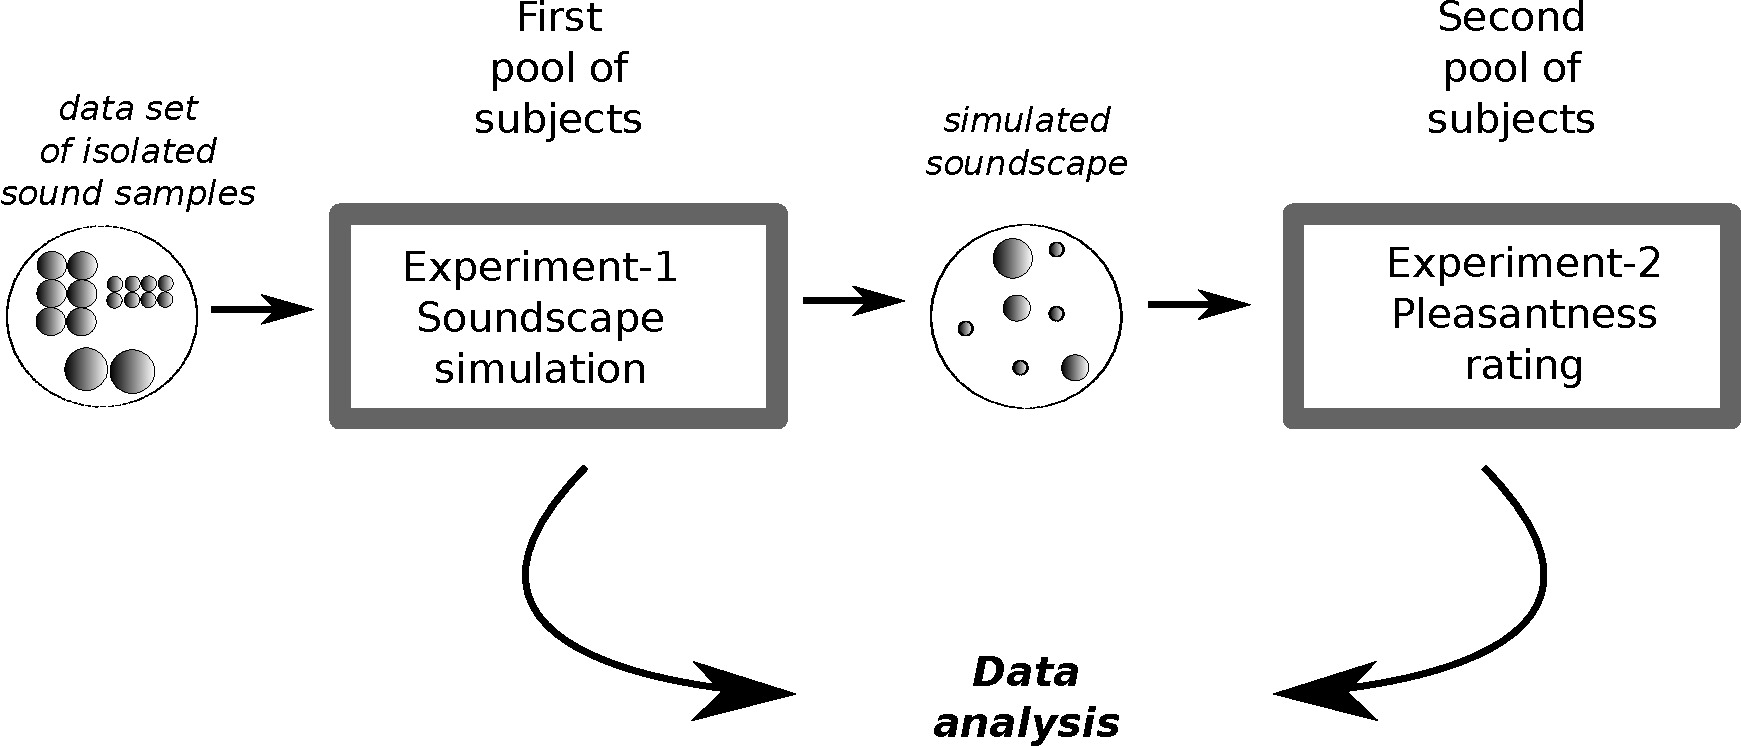
\includegraphics[width=.8\linewidth]{gfx/5}
        \caption{Planification expérimentale des éxperiences de simulation et d'évaluation de l'agrément}\label{fig:xp1_2}
\end{figure}



\subsection{Banque de données de sons isolés}

Dans cette section, nous présentons le processus de sélection et d'acquisition des sons utilisés comme matériau de base lors de la simulation des environnements sonores urbains. La banque de données est identique à celle utilisée dans le cadre de l'expérience pilote \citep{lafay2013atiam,lafay2014new}. 

\jlv{Pour plus de détails sur l'organisation interne de la banque de données, ainsi que sur l'interface graphique permettant de les sélectionner, nous invitons le lecteur à se référer à la section~\ref{sec:db_ui}.}
\jls{Pour plus de détails sur l'organisation interne de la banque de données, ainsi que sur l'interface graphique permettant de sélectionner ces dernières, 
voir~\ref{sec:db_ui}.}
\subsection{Typologie des sources sonores présentes dans l'environnement urbain}

Dans le but de\jls{Afin de} créer un corpus de sons isolés de référence, pour la simulation, nous avons réalisé une typologie des sons environnementaux urbains. 

Pour ce faire, une étude bibliographique est effectuée afin d'identifier les sources et ambiances sonores les plus souvent citées dans la littérature. Cette étude porte sur 16 articles ou thèses. Chacun d'eux traite de la manière dont nous discriminons les paysages sonores urbains. \jlv{Plusieurs approches sont possibles, nous en avons relevés trois} \jls{Il ressort que plusieurs approches sont possibles} :

\begin{itemize}
\item 9 articles abordent le problème par une approche perceptive, soit en identifiant ou répertoriant des catégories de sources sonores, soit en étudiant l'impact de classes de sons spécifiques sur la perception de l'environnement : \cite{maffiolo_caracterisation_1999,raimbault2002simulation,guastavino_etude_2003,defreville2004aactivity,raimbault2005urban,dubois2006cognitive,devergie_relations_2006,guastavino2006ideal,niessen2010categories}
\item 3 articles proposent une classification morpho-typologique, divisant l’environnement sonore urbain en ``\,zones sonores\,'' possédant une identité acoustique forte, selon la configuration et la pratique du site : \cite{maffiolo_caracterisation_1999,beaumont2004pertinence,polack2008perceptive}
\item 2 articles répertorient et classifient les sources sonores d’un point de vue expert : \cite{leobon_analyse_1986,brown2011towards}
\end{itemize}

La nature des classes est établie par rapport aux catégories perceptives, ou classes de sons, les plus souvent citées dans ces papiers \jls{publications}. A  partir des éléments relevés, nous établissons deux taxonomies : une pour les événements (\cf~Figure~\ref{fig:taxonomie}.a), une autre pour les textures (\cf~Figure~\ref{fig:taxonomie}.b). Comme évoqué à la section~\ref{sec:db_ui}, la structure taxonomique de ces deux ensembles s'inspire grandement de l'axe vertical de l'organisation catégorielle \jls{exit:comme} proposée \jlc{proposée se rapporte à "axe vertical" ou à organisation catégorielle ?} par E. Rosch (\Cf~section~\ref{XX}), \ie~plus le niveau d'abstraction de la classe est élevé, plus la description de la classe est précise, et plus les sources sonores incluses dans cette classe sont semblables (\Cf~Figure~\ref{fig:orgDb}). Pour les événements, nous considérons quatre niveaux d'abstraction allant des classes les plus globalisantes (niveau d'abstraction 0) aux classes les plus spécifiques (niveau d'abstraction 3). Pour les textures nous ne considérons que trois niveaux d'abstraction.

La typologie obtenue pour les événements est très similaire à une autre \jls{à cette autre...} typologie de sources sonores présentes en milieu urbain, effectuée postérieurement \citep{Salamon14}. \\

\gl{Vérifier les articles que Salamon utilise pour établir sa typologie}

\begin{figure}[bth]
        \myfloatalign
        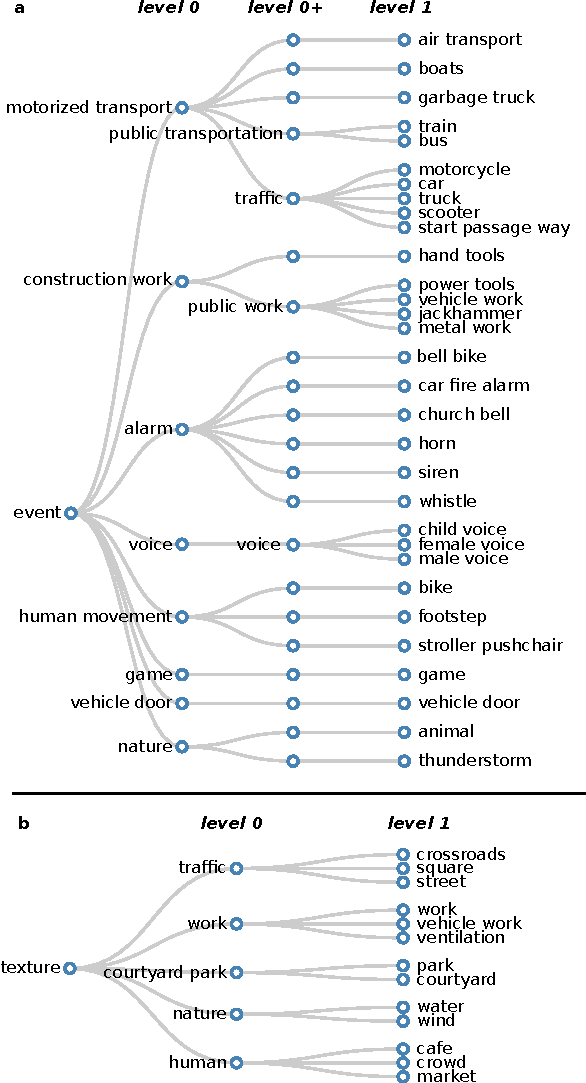
\includegraphics[width=.5\linewidth]{gfxHierarchy/taxonomy}
       \caption[Taxonomies des classes de sons utilisées\jlc{"utilisées" se rapporte à "taxonomies" ?} pour la simulation des environnements sonores urbains]{Taxonomies des classes de sons utilisées pour la simulation des environnements sonores urbains pour (a) les événements sonores et (b) les textures sonores. Nous présentons ici uniquement les niveaux d'abstraction 0 et 1. Un niveau intermédiare, nommé $0+$, et utilisé pour l'analyse, est également introduit.}\label{fig:taxonomie}
\end{figure}

\subsection{Acquisition des sons isolés}

Sur la base des typologies précédemment établies, 483 sons ont été collectés, dont 381 \jls{exit:des} événements et 102 \jlc{exit:des} textures.

Parmi les événements :

\begin{itemize}
\item 260 sont issus d’enregistrements
\item 89 sont issus de la banque de sons \emph{SoundIdeas}\footnote{Pour plus de détails sur \emph{SoundIdeas} voir :\url{ http://www.sound-ideas.com/}}
\item 32 sont issus de la banque de sons \emph{Universal SoundBank}\footnote{Pour plus de détails sur \emph{Universal SoundBank} voir : \url{http://www.universal-soundbank.com/}}
\end{itemize}

Parmi les textures:

\begin{itemize}
\item 72 sont issues d’enregistrements
\item 23 sont issues de la banque de sons \emph{SoundIdeas}
\item 7 sont issues de la banque de sons \emph{Universal SoundBank}
\end{itemize}

\gl{Pour les événements, les regroupements se font en grande majorité par rapport à la source et sont d’ordre sémantique. Pour les textures nous considérons également la nature des lieux hébergeant ces dernières (\eg~\emph{parc}, \emph{rue})}.

Tous les enregistrements ont été effectués à l’aide d'un micro canon \emph{AT8035}\footnote{\Cf~\url{http://eu.audio-technica.com/fr/products/product.asp?catID=1&subID=6&prodID=1845}} relié à un enregistreur \emph{ZOOM H4n}\footnote{\Cf~\url{http://www.zoom.co.jp/english/products/h4n/}}. L’utilisation du micro canon nous permet d’isoler les événements sonores du magma urbain. \jls{exit:Inversement}, pour les textures, il nous permet d’éviter les événements sonores proches du preneur de son, \jls{exit:chose impossible avec un micro omnidirectionnel}. Nous pouvons ainsi pointer des "zones sonores", en nous tenant à une certaine distance de ces dernières afin de capter uniquement le brouhaha émanant de la zone ciblée.

Tous les sons ont été normalisés au même niveau $RMS$ \footnote{Le niveau $RMS$, de l'anglais \emph{Root Mean Square} \jls{qui} désigne la valeur efficace d'un signal. Formellement, le niveau $RMS$ $x_{RMS}$ d'un signal $x=(x_1,x_2,\ldots,x_n)$ s'obtient en calculant la moyenne quadratique de ce dernier $x_{RMS}=\sqrt{\dfrac{1}{n}\sum\limits_{i} x_i^2}$} de $-12$ $dB$ (FS) \footnote{$dB$ (FS) est le sigle anglais désignant une valeur en décibels relative à la pleine échelle (\emph{relative to Full Scale}), \ie~le rapport entre le niveau du signal et sa valeur maximale. Dans notre cas, ce niveau pleine échelle est de 1 Volt.}.

\subsection{Planification expérimentale}

\subsubsection{Épreuve de simulation}
\label{sec:ch5_planExpSimu}

\textbf{Procédure} \\

\jlv{Les sujets doivent simuler deux environnements sonores urbains, chacun devant durée de 1 minute. Pour les deux simulations, les sujets doivent se conformer aux consignes suivantes.}
\jls{Les sujets doivent simuler deux environnements sonores urbains, chacune des scènes devant durer 1 minute. Pour ces simulations, les sujets doivent se conformer aux consignes suivantes:}
\begin{itemize}
\item Première simulation : Simuler un paysage sonore \textbf{urbain plausible} qui selon vous est idéal (où vous aimeriez vivre).
\item Deuxième simulation : Simuler un paysage sonore \textbf{urbain plausible} qui selon vous est non-idéal (où vous n'aimeriez pas vivre).
\end{itemize}

Tous les sujets commencent par simuler l'environnement idéal. Les sujets ne prennent connaissance de la deuxième consigne qu'à la fin de la première simulation.

Les sujets son totalement libres dans le choix des sons, et des paramètres (\Cf~section~\ref{XX} pour plus de détails sur les paramètres) \jls{(pour plus de détails sur les paramètres voir \Cf~section~\ref{XX} je suggère afin de conserver une unité de présentation, cf les références précédemment citées}. Ils doivent cependant \jlv{se conformer} \jls{se soumettre} à deux contraintes:

\begin{itemize}
\item le sujet doit prendre le point de vue d’un auditeur fixe

\item le paysage sonore doit être réaliste au sens de physiquement plausible. Autrement dit, le sujet à tout à fait le droit de placer 10 chiens dans son paysage sonore, mais il n’a pas le droit de placer 1 chien aboyant toutes les 100 millisecondes.

\end{itemize}

Chaque processus de simulation comprend deux parties :

\begin{enumerate}
\item la réalisation de la simulation: cette étape peut, elle même, se décomposer en trois actions (\Cf~section~\ref{XX}):
\begin{itemize}
\item sélectionner les classes de sons
\item nommer les classes de sons sélectionnées
\item paramétrer les pistes (\Cf~section~\ref{XX}) relatives aux classes de sons sélectionnées
\end{itemize}
\item la réalisation d'un commentaire libre du paysage sonore simulé
\end{enumerate}

En complément, et une fois les deux scènes sonores réalisées, le sujet est invité à 

\begin{itemize}
\item indiquer les sources sonores manquantes
\item commenter l’ergonomie du logiciel de simulation
\item commenter l’ergonomie \jlc{de} l'interface de sélection
\end{itemize}

Avant de commencer la première simulation, un petit tutoriel de 20 minutes est proposé aux sujets, afin qu'ils se familiarisent avec le logiciel de simulation, et la banque de données. Le tableau~\ref{tab:indSimu} résume les étapes de l’expérience ainsi que leurs durées respectives. L'expérience est prévue pour durer 2h30. \\

\begin{table}[t]
\centering
\begin{tabular}{c c c} 
Index          & Tâche                               & Durée (min) \\                      
\hline
1 & Présentation de l'expérience                     & 10 \\
  & Lecture de la consigne                           &  \\
\hline
2 & Tutoriel (Réalisation d'une scène test)          & 20 \\
\hline
3 & Première simulation: scène idéale                & 40 \\
\hline
4  & Commentaire de la scène idéale                  & 15 \\
\hline
3 & Deuxième simulation: scène non-idéale            & 40  \\
\hline
4  & Commentaire de la scène non-idéale              & 15 \\
\hline
5 & Critique de l'interface de simulation            & 10 \\
  & et de l'interface de sélection                   & \\
\hline
\end{tabular}
\vspace{0.5mm}
\caption{Résumé des étapes de l’expérience de simulation}
\label{tab:indSimu}
\end{table}

\textbf{Apparatus} \\

Tous les sujets passent l'expérience sur des machines identiques (\gl{description des machines}). L'audio est présenté en stéréophonie, par le biais de casques audio. Pendant le tutoriel, les sujets doivent ajuster le niveau sonore à un volume confortable. Ils ne peuvent le modifier par la suite.

Tous les sujets réalisent l'expérience simultanément. Ils sont répartis de manière égale dans trois pièces identiques, \jlv{toutes possédant} \jls{et offrant toutes...} un environnement calme. Ils n'ont pas le droit de s'adresser la parole pendant l'expérience.

Trois expérimentateurs, un dans chaque pièce, sont présents durant la totalité de l'expérience, afin de contrôler le bon déroulement de cette dernière, et de répondre aux éventuelles questions des sujets.  \\

\textbf{Participants} \\

44 étudiants (14 femmes) de L’École Centrale de Nantes ont participé à l'expérience. Ils ont tous \jlv{un peu près} \jls{sensiblement} le même âge (moyenne: 21.6, écart-type: 2). Tous les sujets ont vécu dans la même ville (Nantes), au minimum pendant les deux dernières années précédant l'expérience.\jlc{ce "au minimum" laisse entendre que ces deux ans constituent une condition préalable à l'expérimentation.} Si c'est le cas \jls{Tous les sujets sont Nantais, et ont vécu dans cette ville durant les deux années, au moins, qui ont précédé l'expérience}. Si au contraire nous sommes sur le registre du constat \jls{Tous les sujets sont Nantais, et vivent dans cette ville depuis deux ans ou plus}. 

\jlv{Dû a une incompréhension des consignes, ou à l'impossibilité de finir dans les temps, 4 sujets ne sont pas pris en compte pour l'analyse. 40 sujets ont réalisés l'expérience avec succès, nous fournissant 80 scènes sonores simulées, 40 idéales, 40 non-idéales.}
\jls{Sur les 44 sujets, 40 réalisent l'expérience avec succès, produisant au final 80 scènes sonores simulées, dont 40 scènes idéales, et 40 scènes non idéales. 4 sont éliminés pour non respect et/ou incompréhension des consignes, d'une part, dépassement du temps, d'autre part.}

\subsubsection{Épreuve d'évaluation de l'agrément}
\label{sec:ch5_planExpEvaA}

\textbf{Procédure} \\

Les sujets doivent évaluer l'agrément des 80 scènes sonores simulées. \jlv{Dû à des contraintes de temps, les sujets n'évaluent que 30 secondes des scènes simulées (à l'origine d'une durée de 1 minute). Ces 30 secondes sont extraites à partir de la 15ème et jusqu'à la 45ème seconde des scènes simulées (ayant à l'origine une durée de 1 minute)}. \jls{En raison de contraintes temps, les sujets n'évaluent que des séquences de 30 secondes des scènes simulées, chacune de ces séquences commençant à la seconde 15, et finissant à le seconde 45, de la scène évaluée.}

L'évaluation s'effectue sur une échelle sémantique bipolaire de 7 points allant de -3 (non-idéale/très désagréable) à +3 (idéale/très agréable). Avant de noter une scène, les sujets doivent obligatoirement écouter les 20 premières secondes de cette dernière. Après la notation, ils sont libres de passer à la scène suivante \jls{ exit:, avant la fin des 30 secondes}.

Pour chaque sujet, les scènes sont présentées dans un ordre aléatoire. Les dix \jls{Les 10} \jlc{depuis un moment on parle en chiffres je suggère de continuer pour l'unité} premières scènes permettent au sujet d'ajuster ses notes. Elles sont obligatoirement composées de 5 scènes idéales et de 5 non-idéales. Ces dix \jls{10} premières scènes sont rejouées à la fin de l'expérience, et seules les notes données à la deuxième occurrence sont prises en compte. \\

\textbf{Apparatus} \\

Tous les sujets passent l'expérience sur des machines identiques (\gl{description des machines}). L'audio est présenté en stéréophonie, par le biais de casques audio semi-ouvert \emph{Beyer-Dynamic DT 990 Pro}. Toutes les scènes sonores ont été re-simulées sur la base des partitions (\gl{citer section décrivant le terme partition}) obtenues lors de l'expérience de simulation. Le niveau sonore de sortie est identique pour tous les sujets.

Tous les sujets réalisent l'expérience simultanément, dans un environnement calme. Ils n'ont pas le droit de s'adresser la parole pendant l'expérience. 


Un expérimentateur est présent durant la totalité de l'expérience, afin de contrôler le bon déroulement de cette dernière, et de répondre aux éventuelles questions des sujets.  \\

\textbf{Participants} \\

10 étudiants (2 femmes) de L’École Centrale de Nantes ont participé à l'expérience. Aucun d'entre eux n'a réalisé l'expérience de simulation. Tous les sujets ont \jlv{un peu près} \jls{sensiblement} le même âge (moyenne: 23.1, écart-type: 1.8). \jlv{Tous les sujets ont vécu dans la même ville (Nantes), au minimum pendant les deux dernières années précédant l'expérience.} \jls{Tous les sujets sont Nantais, et vivent dans cette ville depuis deux ans ou plus}

Tous les sujets ont réalisé l'expérience avec succès.

\subsection{Données et méthodes d'analyses}

\subsubsection{Nature des données analysées}

\jlv{De toutes les données produites par l'épreuve de simulation, nous analysons:} 
\jls{A partir des données produites par l'épreuve de simulation, nous analysons:}

\begin{itemize}
\item les partitions des scènes simulées (\Cf~section~\ref{XX})
\item les signaux des scènes simulées
\item les commentaires sur les sons manquants et l'ergonomie des interfaces de simulation et de sélection
\end{itemize}

Chaque scène est décrite par un groupe de descripteurs. C'est sur la base de ces descripteurs que nous pratiquons l'analyse. Un résumé des descripteurs, ainsi que des acronymes les désignant est présenté dans le Tableau~\ref{tab:acronyme}. Afin de rester cohérent avec l'épreuve d'évaluation, les descripteurs issus des partitions ou des signaux des scènes ne sont pas calculés sur la durée totale \jlv{des scènes} \jls{de celles-ci}, mais sur une version réduite de 30 secondes (\Cf~section~\ref{sec:ch5_planExpEvaA}). 

Pour chaque scène sonore, trois types de descripteurs sont considérés:

\begin{itemize}
\item \emph{Perceptif}: Il s'agit de l'agrément perçu \jlv{des scènes simulées} \jlc{Dans ce passage, nous décrivons les descripteurs considérés au niveau de chaque scène. Peut-être devrions nous employer le singulier: "de la scène simulée", et retrouver ainsi une unité avec les items suivant ?}, évalué sur une échelle sémantique 7 points. Nous notons $A$ l'agrément moyen d'une scène, obtenu en moyennant les notes de tous les sujets. Considérant le faible nombre de sujets, nous faisons le choix, dans cette étude, de ne pas normaliser les notes d'agrément.
\item \emph{Sémantique}: Il s'agit d'un vecteur booléen noté $S=(x_1,x_2,\ldots,x_n)$ indiquant les classes de sons présentes dans la scène. Chaque point $x$ de ce vecteur correspond à une classe de sons particulière: $x=1$ si la classe est présente dans la scène, et $x=0$ autrement. La dimension $n$ des vecteurs dépend du niveau d'abstraction considéré, \eg~pour le niveau d'abstraction 1, qui comprend $44$ classes de sons, cette dimension sera de $n=44$.
\item \emph{Structurel}: Les descripteurs structurels sont calculés à partir des partitions et des signaux des scènes simulées. Trois descripteurs structurels sont envisagés:
\begin{itemize}
\item \emph{Diversité} ($DIV$) : Il s'agit d'un scalaire représentant la diversité des classes sonores utilisées pour simuler une scène. Nous calculons $DIV$ en comptant le nombre de classes de sons distinctes utilisées pour une simulation. Ce nombre dépend du niveau d'abstraction considéré. Considérons les deux sous classes du niveau d'abstraction 2 \emph{passage de voiture} et \emph{démarrage de voiture}, toutes deux appartenant à la classe \emph{voiture} du niveau d'abstraction 1. Nous comptons deux classes pour la diversité des niveaux d'abstraction 2 et 1, et seulement une pour les niveaux d'abstraction 0 et 1.
\item \emph{Densité} ($D$) : Il s'agit d'un scalaire représentant le nombre de sources sonores présentes en moyenne. Pour obtenir $D$, nous calculons le logarithme du nombre d'éléments sonores par fenêtre de 125 millisecondes (sans recouvrement), et moyennons au cours du temps. Le calcul de $D$ peut inclure toutes les sources sonores de la scène, ou seulement une partie. Dans ce cas, les fenêtres ne contenant pas de sources sonores ne sont pas prises en compte. Nous notons $D(E)$ et $D(T)$ les densités calculées en considérant séparément les sources d'événements et de textures sonores \jlc{exit:respectivement}.
\item \emph{Niveau Sonore} ($L$) : Pour représenter le niveau sonore, nous nous inspirons de la mesure $L_{Aeq}$. Dans notre cas, il s'agit d'un scalaire, calculé sur le signal en volts, et non en pression, et donné en décibels en prenant un référentiel de 1 Volt. Le niveau est obtenu en calculant, toutes les secondes, la moyenne quadratique du signal, et en moyennant sur la durée de la scène. Un filtrage de type A est opéré avant le calcul des moyennes quadratiques. D'autre descripteurs, inspirés eux aussi de descripteurs acoustiques classiques ($L_{Amin}$, $L_{Amax}$, $L_{A10-90}$), et utilisant un opérateur autre que la moyenne (minimum, maximum, les 10-90ème quantiles) pour intégrer les fenêtres de 1 seconde,  ont été testés. Mais, ces derniers présentant tous une corrélation élevée avec $L$ ($r_{pearson}\geq0.76$, $p<0.01$), \jlv{nous conservons uniquement ce dernier comme descripteur objectif du niveau sonore.} \jls{nous conservons le scalaire ci-devant mentionné comme unique descripteur objectif du niveau sonore}.
\end{itemize}
\end{itemize}

\begin{table}[t]
\centering
\begin{tabular}{c c} 
descripteurs et         & Acronymes  \\       
termes couramment utilisés & \\                
\hline
Densité de sources sonores    & $D$  \\
Densité d’événements sonores & $D(E)$ \\
Densité de sources sonores   & $D(T)$ \\
Niveau sonore globale        & $L$  \\
Niveau sonore calculé        & $L(E)$ \\
sur les événements           &      \\
Niveau sonore calculé        & $L(T)$ \\
sur les textures             &      \\
Diversité de classe          & $DIV$   \\
de sons                      &         \\
Diversité de classe          & $DIV(E)$\\
de sons d'événements         &         \\
Diversité de classe          & $DIV(T)$\\
de sons de textures          &      \\
sur les sujets               &      \\
Agrément par scène           & $A$  \\
(moyenné sur les sujets)     &      \\
\hline
idéale/agréable                & i \\
non-idéale                    & ni \\
scène idéale/agréable         & i-scène \\
scène non-idéale/désagréable  & ni-scène \\
\hline
\end{tabular}
\vspace{0.5mm}
\caption{TODO}
\label{tab:acronyme}
\end{table}

\subsubsection{Méthodologie et Outils statistiques}
\label{sec:ch5_methodoEtStat}

Afin d'évaluer l'impact spécifique des différentes sources sonores sur l'agrément perçu, \jlv{nous divisons l'étude en suivant 6 sous-objectifs} \jls{:nous soumettons nos travaux aux six tests/études de significativité présentés ci-après:}
\jlc{Dans la présentation des item qui suit, je m'attache surtout à conserver une unité de présentation: Afin de... Nous faisons... A TOI DE VERIFIER SI TOUT CELA RESTE PERTINENT}
\begin{itemize}
\item \emph{Étude qualitative} : Afin de vérifier la validité écologique de 1) la banque de données et 2) l'interface de sélection, nous réalisons une étude qualitative des critiques ergonomiques effectuées par les sujets.
\item \emph{Étude comparative entre les descripteurs structurels} : \jlv{Il s'agit ici d'évaluer si la distinction affective imposée entre les i- et ni-scènes impacte de manière significative la nature des scènes, \ie~si il existe des différences significatives entre les descripteurs structurels et/ou l'agrément perçu. La significativité est évaluée à partir d'un test de Student à deux échantillons appariés (\Cf~Annexe~\ref{app:statuni}).} \jls{Afin d'évaluer si la distinction affective imposée entre les i- et ni-scènes impacte de manière significative la nature des scènes, \ie~si il existe des différences significatives entre les descripteurs structurels et/ou l'agrément perçu, nous évaluons cette significativité à partir d'un test de Student à deux échantillons appariés (\Cf~Annexe~\ref{app:statuni}).}
\item \jlv{\emph{Influence des descripteurs structurels sur l'agrément perçu}} \jls{Etude de l'influence des descripteurs structurels sur l'agrément perçu}: \jlv{Nous adoptons ici une méthodologie couramment utilisée dans l'approche dimensionnelle. Pour évaluer l'impact potentiel des descripteurs structurels sur l'agrément perçu, nous étudions l'existence de corrélation linéaire entre entre ces deux types de descripteur. Pour mesurer la corrélation, nous utilisons le coefficient de Pearson (\Cf~Annexe~\ref{app:statuni}).} \jls{Afin d'évaluer l'impact potentiel des descripteurs structurels sur l'agrément perçu, nous étudions l'existence de corrélation linéaire entre entre ces deux types de descripteurs. Pour mesurer la corrélation, nous utilisons le coefficient de Pearson (\Cf~Annexe~\ref{app:statuni}). Nous adoptons ici une méthodologie couramment utilisée dans l'approche dimensionnelle.}
\item \emph{Étude comparative entre les descripteurs sémantiques}: \jlv{Il s'agit ici d'apprécier si la distinction affective imposée a eu un impact sur la composition des scènes en terme de sources sonores. Plus précisément, il s'agit d'observer si il existe des classes de sons qui ont été particulièrement utilisées pour simuler un type d'environnement. Nous utilisons le V-test, afin de tester si la présence d'une classe de son est typique d'un environnement (i ou ni). Le test est effectué pour chaque niveau d'abstraction et séparément pour les classes d'événements et de textures. Pour chaque classe $j$ et chaque type d'environnement $k$ ($k={i,ni}$), la valeur $V_{jk}$ du V-test se calcule comme suit} \jls{Afin d'apprécier si la distinction affective imposée a eu un impact sur la composition des scènes en terme de sources sonores, ou, pour être plus précis, s'il existe des classes de sons qui ont été particulièrement utilisées pour simuler un type d'environnement, nous utilisons le V-test. Nous vérifions si la présence d'une classe de sons est typique d'un environnement (i ou ni). Le test est effectué pour chaque niveau d'abstraction, et séparément pour les classes d'événements et de textures. Pour chaque classe $j$ et chaque type d'environnements $k$ ($k={i,ni}$), la valeur $V_{jk}$ du V-test se calcule comme suit:} 

\begin{equation*}
V_{jk}=\dfrac{n_{jk}-n_k\frac{n_j}{n}}{\sqrt{n_k}\frac{n-n_k}{n-1}\frac{n_j}{n}(1-\frac{n_j}{n})}
\end{equation*}

avec $c$ le nombre de classes utilisées, $c_k$ le nombre de classes utilisés pour un type d'environnements $k$, $c_j$ le nombre de classes $j$ utilisées, et $c_{jk}$ le nombre de classes $j$ utilisées pour un type d'environnements $k$. Le V-test teste l'hypothèse nulle que la proportion $\frac{c_{jk}}{c}$ ne diffère pas significativement de la proportion $\frac{c_{jk}}{c_k}$. Si pour un environnement $k$ et une classe $j$ l'hypothèse est rejetée, la classe $j$ est alors typique de l'environnement $k$. Les classes typiques sont nommées \textbf{les marqueurs sonores}.

\item \emph{Étude des espaces de représentations induits par les descripteurs sémantiques}: \jlv{Dans cette analyse, nous étudions si une représentation basée uniquement sur la présence ou l'absence des classes de sons permet de séparer les deux types d'environnements} \jls{Afin d'étudier si une représentation basée uniquement sur la présence ou l'absence des classes de sons permet de séparer les deux types d'environnements}. Pour ce faire, nous considérons l'espace induit par les descripteurs sémantiques $S$. $S$ étant un vecteur booléen, nous calculons les distances entre les scènes à partir de la distance de \emph{hamming}. Considérant les deux vecteurs $S_1=(x_{1,1},x_{1,2},\ldots,x_{1,n})$ et $S_2=(x_{2,1},x_{2,2},\ldots,x_{2,n})$ de dimension $n$, avec $x={0,1}$, la distance de \emph{Hamming} $d_{ham}$ mesure le pourcentage de coordonnés qui diffèrent entre les deux vecteurs.    


\begin{equation*}
d_{ham}(S_1,S_2)=\dfrac{1}{n}\sum_{i=1}^{n} (x_{1,i} \bigoplus x_{2,i})
\end{equation*}

où $\bigoplus$ désigne l'opérateur du \emph{ou-exclusif}. Plus la composition des deux scènes est similaire, et plus ces deux scènes seront proches. L'utilisation de la distance de \emph{Hamming} permet de prendre en compte de manière égale les classes présentes et absentes. Pour mesurer la capacité intrinsèque de l'espace à séparer les i- et ni-scènes, nous utilisons une métrique de \emph{clustering} nommée précision au rang $k$ ($p@k$). Pour calculer la $p@k$, nous regardons d'abord, pour chaque item, le taux d'items \jlc{le "pour chaque item le taux d'items" est mal dit. Il faut trauver une autre formulation. Perso je ne peux pas t'aider} partageant le même label parmi ses $k$ plus proche(s) voisin(s). La $p@k$ est alors la moyenne des taux pour tous les items.

\item \jlv{\emph{Influence spécifique marqueurs sonore sur l'agrément perçu}} \jls{Etude de l'influence spécifique des marqueurs sonores sur l'agrément perçu}: \jlv{Une fois les marqueurs sonores identifiés, nous évaluons une nouvelle fois l'impact potentiel des descripteurs structurels sur l'agrément perçu, mais en ne tenant compte cette fois que des marqueurs sonores pour calculer ces descripteurs} \jls{Afin, les marqueurs sonores étant identifiés, d'évaluer une fois encore l'impact potentiel des descripteurs structurels sur l'agrément perçu, en ne tenant compte, cette fois, cependant, que des marqueurs sonores pour calculer ces descripteurs.}
\end{itemize}

Excepté le V-test, tous les tests de significativité sont effectués avec un seuil critique $\alpha=0.05$. Pour le V-test, étant donné que nous testons beaucoup de classes, une correction de Bonferroni \gl{ref} est appliquée. Concernant les valeurs $p$, dans le cas ou la valeur $p\geq0.05$, nous indiquons sa valeur. Dans le cas ou $0.01\leq p<0.05$, nous indiquons seulement $p<0.05$. Dans le dernier cas nous indiquons $p<0.01$.

Concernant l'interprétation du coefficient de corrélation de Pearson adoptée dans ce document, nous invitons le lecteur à se référer à l'Annexe~\ref{app:corr}.

\subsection{Validité écologique de l'expérience}

\subsubsection{Diversité de la banque de sons}

\jlv{Nous cherchons, dans un premier temps, à vérifier que \jlc{Ce "Dans un premier temps" annonce d'autres temps dans la suite du texte. Or ces temps n'apparaissent pas...} la diversité des classes de sons proposées dans la banque de données est suffisante, afin de pouvoir simuler un environnent sonore. En analysant les commentaires des sujets portant sur la banque données, nous remarquons que 63\% d'entre eux indiquent avoir été au moins une fois dans l'incapacité de trouver un son, avec un maximum de 4 sons par sujet. Parmi tous les sons manquants relevés, nous identifions 26 classes de sons. Parmi ces 26 classes de sons manquantes:}
\jls{Nous voulons vérifier la diversité des classes de sons proposées est suffisante, pour pouvoir simuler un environnent sonore. Nous analysons les commentaires des sujets sur la banque de données. 63\% d'entre eux indiquent avoir été, au moins une fois, dans l'incapacité de trouver un son, avec un maximum de 4 sons par sujet. Parmi les sons manquants relevés, nous identifions 26 classes de sons dont:}
\begin{itemize}
\item 16 sont bien présentes dans la banque de données, l'incapacité des sujets à les trouver n'étant donc pas imputable à la diversité de la base.
\item 1 fait référence à des sons de musique, que nous avons choisi délibérément d'occulter.
\item 9 sont effectivement absentes.  
\end{itemize}

\jlv{Parmi les 9 classes de sons identifiées comme manquantes, nous observons que ces classes sont très spécifiques (\eg~\emph{voiture de sport} ou \emph{voix d'adolescent}), et peuvent être remplacées par des classes similaires (\eg~\emph{voiture} ou \emph{voix d'enfant} ou \emph{voix d'adulte}). Nous pensons que ces résultats montrent que la diversité proposée par la banque de sons est suffisante dans le cadre de notre étude} \jls{Concernant ces dernières, nous observons qu'il s'agit de classes très spécifiques (\eg~\emph{voiture de sport} ou \emph{voix d'adolescent}), et qui peuvent être remplacées par des classes similaires (\eg~\emph{voiture} ou \emph{voix d'enfant} ou \emph{voix d'adulte}). Nous en concluons que la diversité proposée par la banque de sons est suffisante dans le cadre de notre étude}.


\subsubsection{Ergonomie de l'interface de sélection}

\jlv{En considérant les retours sur l'interface de sélection, nous observons que $32.5\%$ des sujets ont spontanément indiqué que l'interface était un moyen ``\,simple et efficace\,'' de sélectionner des sons sans l'aide de texte. $57.5\%$ des sujets n'ont pas fait mention de difficulté particulière. Seulement $10\%$ des sujets ont signalé avoir rencontré des difficultés avec l'interface, mais sans que ces dernières aient sensiblement affecté la simulation} \jls{Nous voulons vérifier l'efficience de l'interface de sélection. Nous analysons les retours des sujets. $32.5\%$ d'entre eux indiquent} \jlc{exit:spontanément} \jls{que l'interface est un moyen ``\,simple et efficace\,'' de sélectionner des sons sans l'aide de texte. $57.5\%$ ne font pas mention de difficultés particulières, $10\%$ signalent enfin avoir rencontré des difficultés avec l'interface, sans toutefois que la simulation en ait été affectée.} 

Ces résultats tendent à montrer que l'interface de sélection sans texte n'a pas perturbé \jls{ne perturbe pas} les sujets outre mesure. Des conclusions similaires ont été obtenues lors de l'expérience pilote \citep{lafay2013atiam,lafay2014new}. \\
\jls{Nous en concluons que l'interface de sélection sans texte ne perturbe pas les sujets outre mesure. Un même constat avait été tiré de l'expérience pilote \citep{lafay2013atiam,lafay2014new}. \\}.
\gl{vérifier une dernière fois}

\subsubsection{Ergonomie de l'interface de simulation}

\gl{to do}

\subsection{Vérification de l'agrément des scènes simulées}

Nous analysons ici l'agrément perçu des $80$ scènes sonores simulées. 

La Figure~\ref{fig:xp2_Aa} affiche l'agrément moyen $A$ pour les i- et ni-scènes. \jlv{Afin de garantir la cohérence de nos données, nous voulons, dans un premier temps, nous assurer qu'aucune ni-scène n'ait un $A$ supérieur à celui d'une i-scène. Nous observons que quatre scènes ne respectent pas cette contrainte. Ces scènes, ainsi que leurs correspondantes i ou ni, sont supprimées de l'analyse. 36 i-scènes et 36 ni-scènes sont conservées dans la suite de l'analyse.} \jls{Dans un premier temps, et afin de garantir la cohérence de nos données, nous voulons nous assurer qu'aucune ni-scène n'ait un $A$ supérieur à celui d'une i-scène. Quatre des scènes ne respectent pas la contrainte. Elles et leurs correspondantes i ou ni sont retirées. 36 i-scènes et 36 ni-scènes restent dans le champ de l'analyse.}

Dans un deuxième temps, nous \jlv{testons} \jls{voulons tester} si les sujets ont bien perçu une différence d'agrément entre les i- et ni-scènes. Pour ce faire, nous observons l'agrément moyen de chaque sujet, calculé séparément pour chaque type d'environnement (\Cf~Figure~\ref{fig:xp2_Ab}). \jlv{Il est clair} \jls{Il apparaît} que les i-scènes ont bien été perçues comme significativement plus agréables ($p<0.01$) que les ni-scènes.

\begin{figure}[t]
        \myfloatalign
        \subfloat[]
        {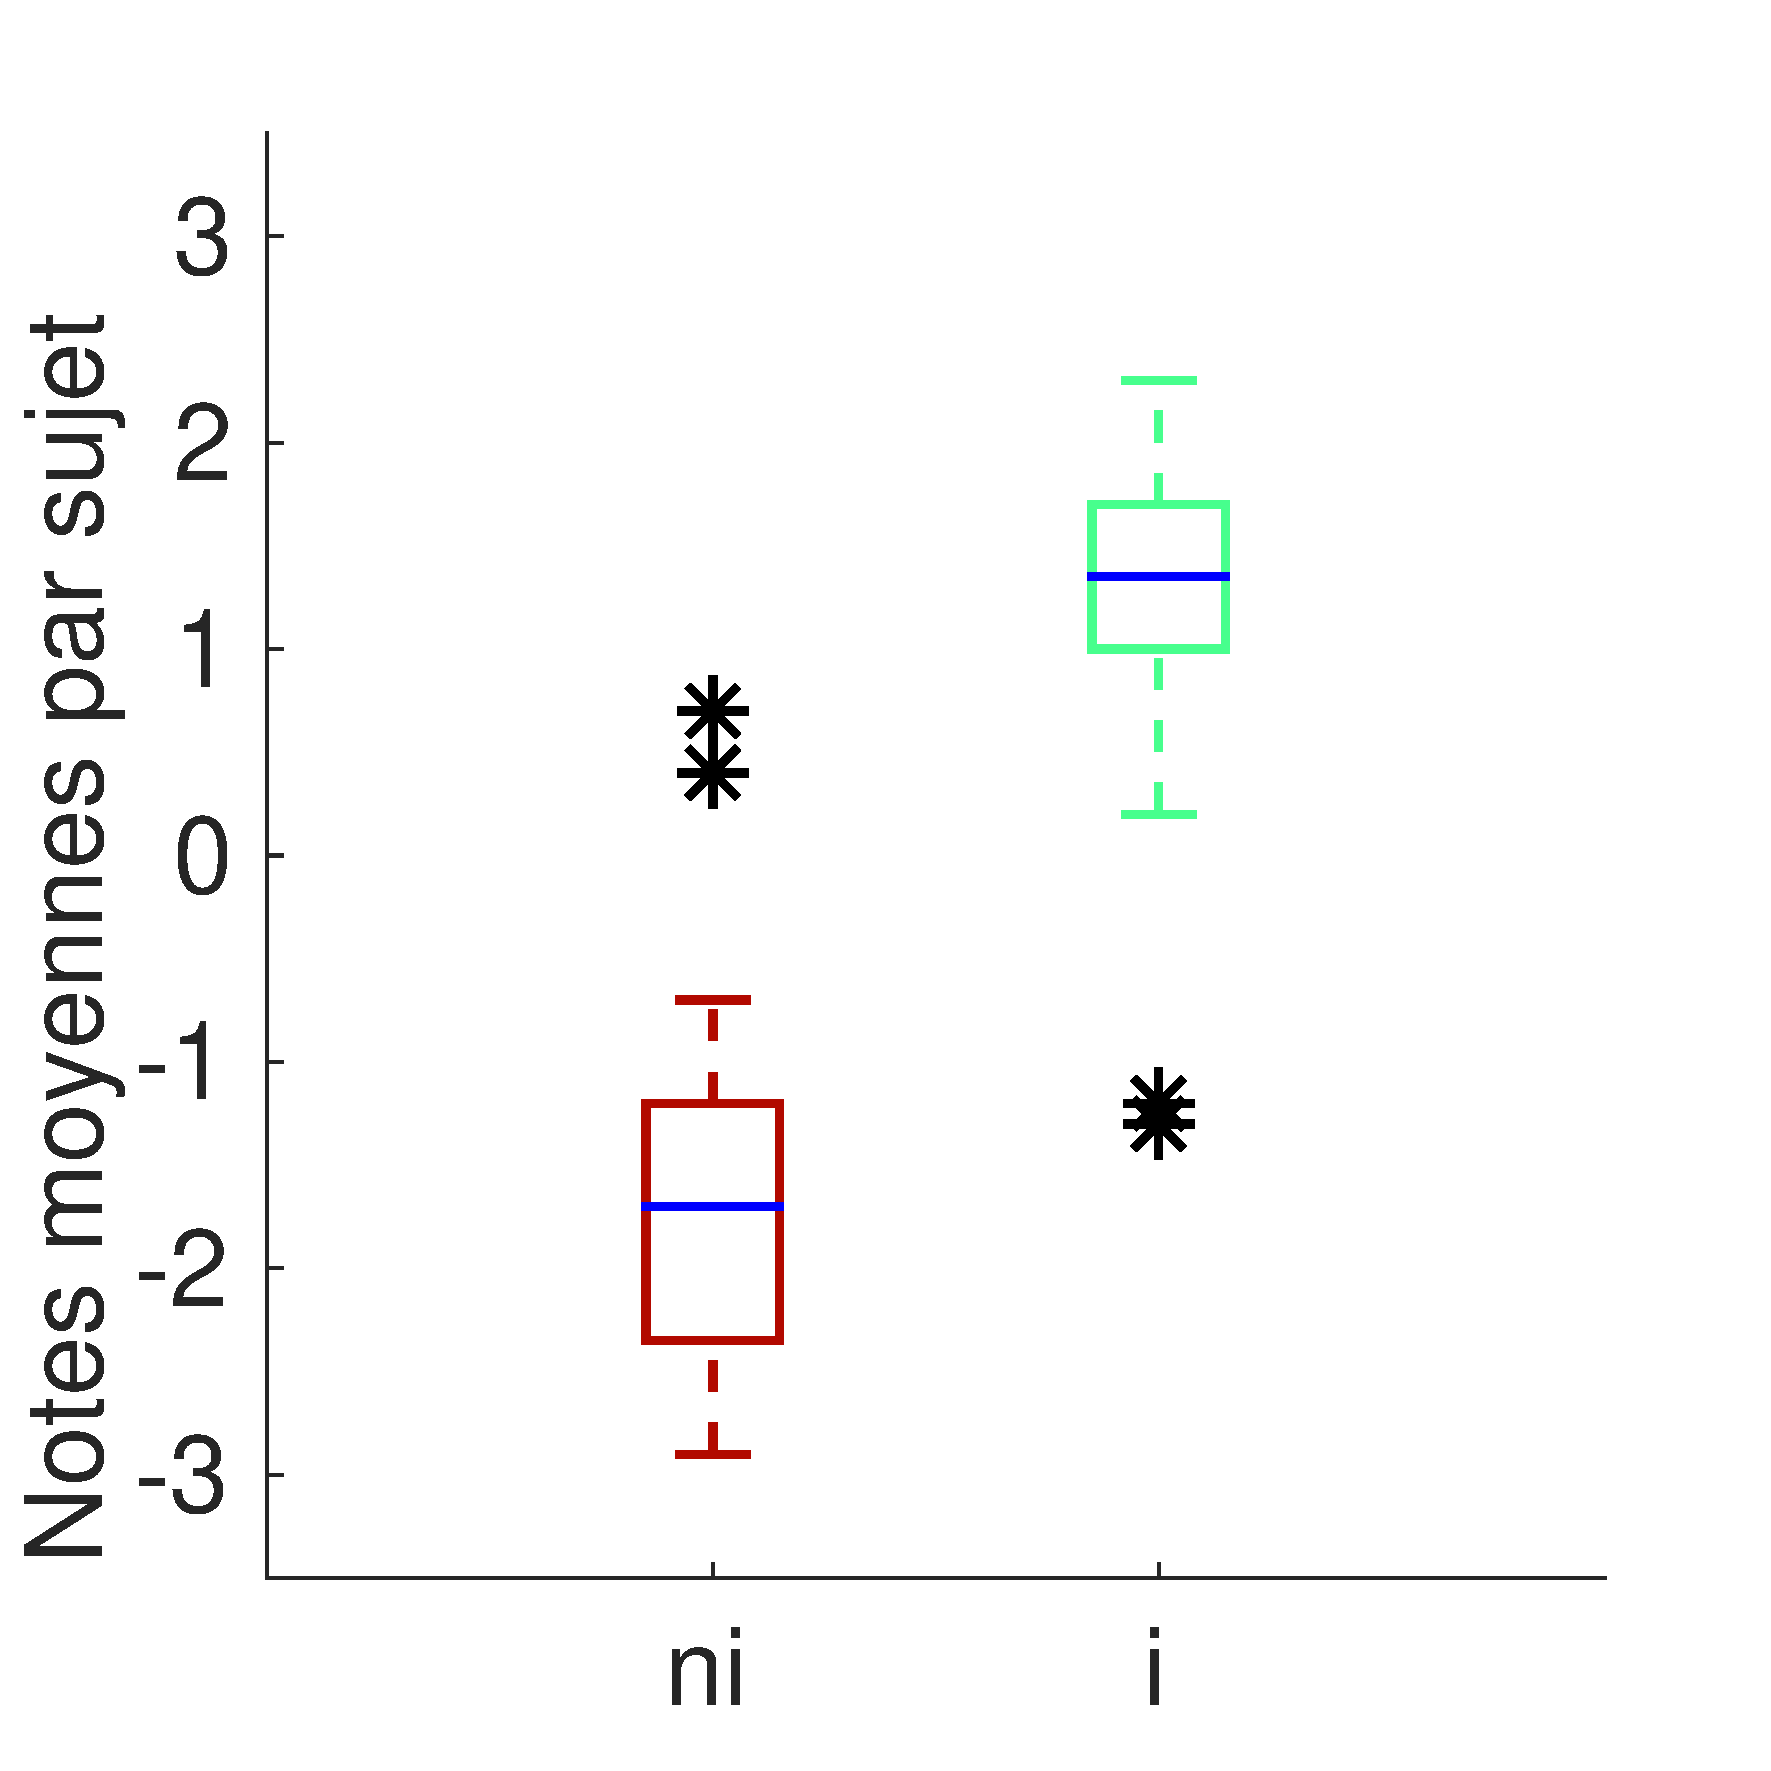
\includegraphics[width=.4\linewidth]{gfxXpUrbanSoundscape/xp2_1}\label{fig:xp2_Aa}}
        \subfloat[]
        {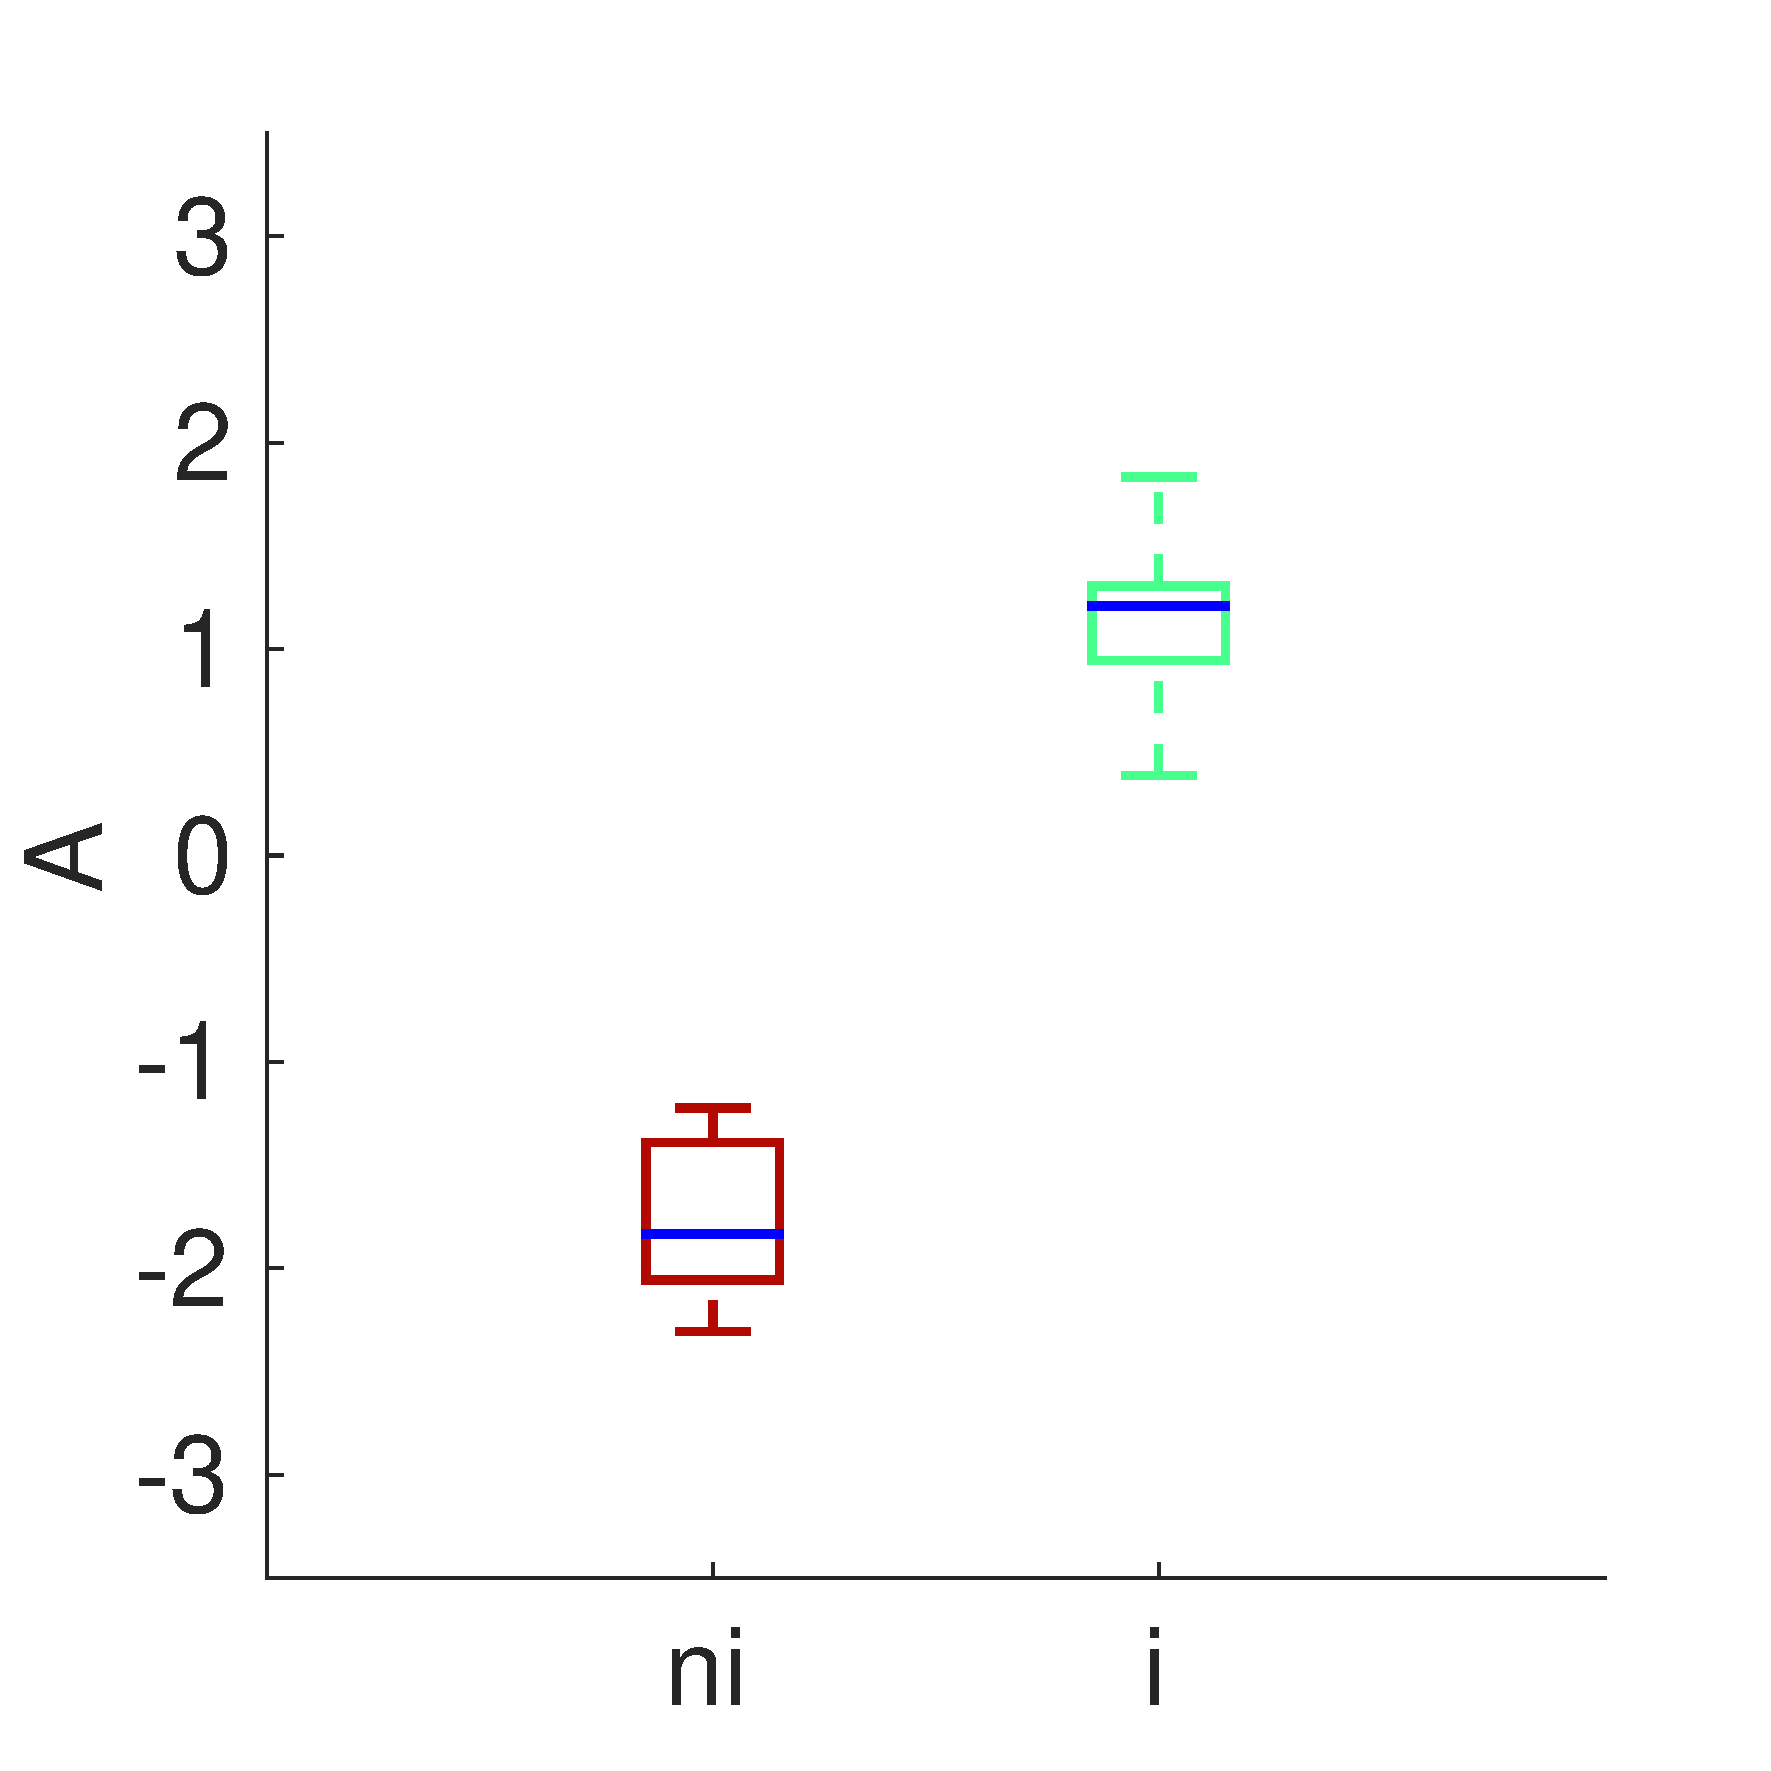
\includegraphics[width=.4\linewidth]{gfxXpUrbanSoundscape/xp2_2}\label{fig:xp2_Ab}}
       \caption[TODO]{TODO}\label{fig:xp2_A}
\end{figure}
 
\subsection{Étude comparative entre les descripteurs structurels}

En premier lieu, nous nous concentrons sur le niveau sonore. Les figures~\ref{fig:soundlevela},~\ref{fig:soundlevelb} et~\ref{fig:soundlevelc} affichent les distributions des niveaux $L$, $L(E)$ et $L(T)$ \jlc{exit:respectivement}. Il existe bien une différence de niveaux significative entre les i- et ni-scènes ($L$: $p<0.01$), avec un écart moyen de -7 $dB$ \jlc{exit:entre ces dernières}. Cette différence affecte aussi bien les événements ($L(E)$: $p<0.01$, écart moyen: -7 $dB$) que les textures ($L(T)$: $p<0.01$, écart moyen: -6 $dB$). 

Nous vérifions \jlc{exit:ici}, sans surprise, que le niveau des sources sonores est bien un indicateur d'agrément, les ni-scènes ayant tendance à être plus fortes. \jlv{Par ailleurs} \jls{Nous constatons encre que...}, cette différence de niveaux s'observe de manière égale pour les événements et les textures sonores. 

Il apparaît que ce sont les événements qui impactent le plus le niveau global des scènes, l'écart entre $L$ et $L(E)$ n'étant que de 1 $dB$ pour les i-scènes et les ni-scènes. Cette observation fait écho aux résultats obtenus par Kuwano~\al \citep{kuwano_memory_2003}. \jlv{Dans un premier temps, les auteurs demandent à un panel \jlc{exit:de sujets} d'évaluer de manière globale une série d'environnements sonores. Dans un deuxième temps, les sujets doivent, pour les mêmes environnements, évaluer le niveau aux instants où ils identifient une source sonore. L'étude montre qu'il n'y a pas de différences significatives entre les jugements globaux et les moyennes des jugements instantanés. On peut penser que nos sujets ont inconsciemment tenu compte de cette réalité perceptive lors de la simulation, en faisant porter le niveau sonore global par des sons courts et bien identifiés, \ie~les événements.} \jls{Au cours de leur expérience, les auteurs demandent à leurs sujets d'évaluer une série d'environnements sonores d'abord de manière globale, ensuite, d'en évaluer le niveau aux instants où chacun identifie une source sonore. L'étude montre qu'il n'y a pas de différences significatives entre les jugements globaux et les moyennes des jugements instantanés}. Pour revenir à nous, c'est comme si nos propres sujets avaient inconsciemment tenu compte de cette réalité perceptive lors de la simulation, en faisant porter le niveau sonore global par des sons courts et bien identifiés, \ie~les événements.

Nous observons enfin que le niveau seul ne permet pas de clairement faire la distinction entre les différents types d'environnements. En effet, $20\%$ des i-scènes ont un niveau supérieur au niveau minimal des ni-scènes, alors qu'il n'y a pas de recouvrement, si l'on considère l'agrément perçu $A$.

\jlv{Nous considérons maintenant les densités de sources sonores} \jls{en second lieu, nous nous penchons sur les densités de sources sonores}. Les Figures~\ref{fig:densitya} et~\ref{fig:densityb} affichent les distributions de $D$ et $D(E)$. Que l'on prenne en compte toutes les sources, ou uniquement les événements, la densité est significativement plus élevée pour les ni-scènes ($D$: $p<0.01$, $D(E)$: $p<0.01$). Nous observons un écart moyen de $+0.36$ pour $D$ (soit en moyenne 2.3 sources sonores par fenêtre de plus pour les ni-scènes), et de $+0.32$ pour $D(E)$ (soit en moyenne 2.1 sources sonores par fenêtre de plus pour les ni-scènes). Si ces écarts sont très similaires \jlc{exit:entre $D$ et $D(E)$}, c'est que la densité des textures ne varie pas de manière significative entre les i- et ni-scènes ($D(T)$: $p<0.08$), l'écart moyen étant de $+0.17$ (soit en moyenne 0.7 sources sonores par fenêtre de plus pour les ni-scènes), \jlc{et} l'écart médian étant quant à lui nul.

Nous constatons ici que la densité peut être un indicateur de qualité, si l'on considère uniquement les événements sonores. Comme pour les niveaux sonores, la densité ne permet pas de clairement séparer les i- et ni-scènes,  $43\%$ des i-scènes ayant un $D(E)$ supérieur à la densité d'événement minimale des ni-scènes.

\jlv{Pour finir, nous nous intéressons à la diversité} \jls{En dernier lieu, nous nous intéressons à la diversité}. Nous affichons sur la figure~\ref{fig:diversity} $DIV$ pour les événements et les textures, en séparant les différents niveaux d'abstractions. Excepté pour le niveau d'abstraction 0, la diversité de classes d'événements sonores est plus élevée pour les ni-scènes ($DIV$ niveaux 1,2 et 3: $p<0.01$ ), avec en moyenne 2 classes présentes en plus. Aucune différence significative n'est observée pour les textures.

\jlv{Les tendances globales observées tendent à montrer qu'un environnement sonore non-idéal est plus fort, plus dense et composé d'une plus grande variété d'événements sonores. Par ailleurs ce sont les caractéristiques des événements, plus que celles des textures, qui semblent porter la distinction entre les i- et ni-scènes. Cependant, aucun de ces \jlc{le "ces" renvoie à des descripteurs dont on aurait déjà parlé, mais quels sont-ils?} descripteurs ne permet, seul, de faire une distinction nette entre les deux types d'environnements, distinction qui pourtant, est perçue de manière non ambiguë par les sujets.} 
\jls{Les tendances globales observées montrent, d'une part, qu'un environnement sonore non-idéal est plus fort, plus dense et composé d'une plus grande variété d'événements sonores qu'un environnement sonore idéal. Elles montrent, d'autre part, que ce sont les caractéristiques des événements, plus que celles des textures, qui semblent porter la distinction entre les i- et ni-scènes. Cependant, aucun des descripteurs ne permet, à lui seul, de faire une distinction nette entre les deux types d'environnements, distinction pourtant perçue de manière non ambiguë par les sujets.}
\begin{figure}[t]
        \myfloatalign
        \subfloat[]
        {\includegraphics[width=.33\linewidth]{gfxXpUrbanSoundscape/xp_soundlevel_1}\label{fig:soundlevela}}
        \subfloat[]
        {\includegraphics[width=.33\linewidth]{gfxXpUrbanSoundscape/xp_soundlevel_3}\label{fig:soundlevelb}}
        \subfloat[]
        {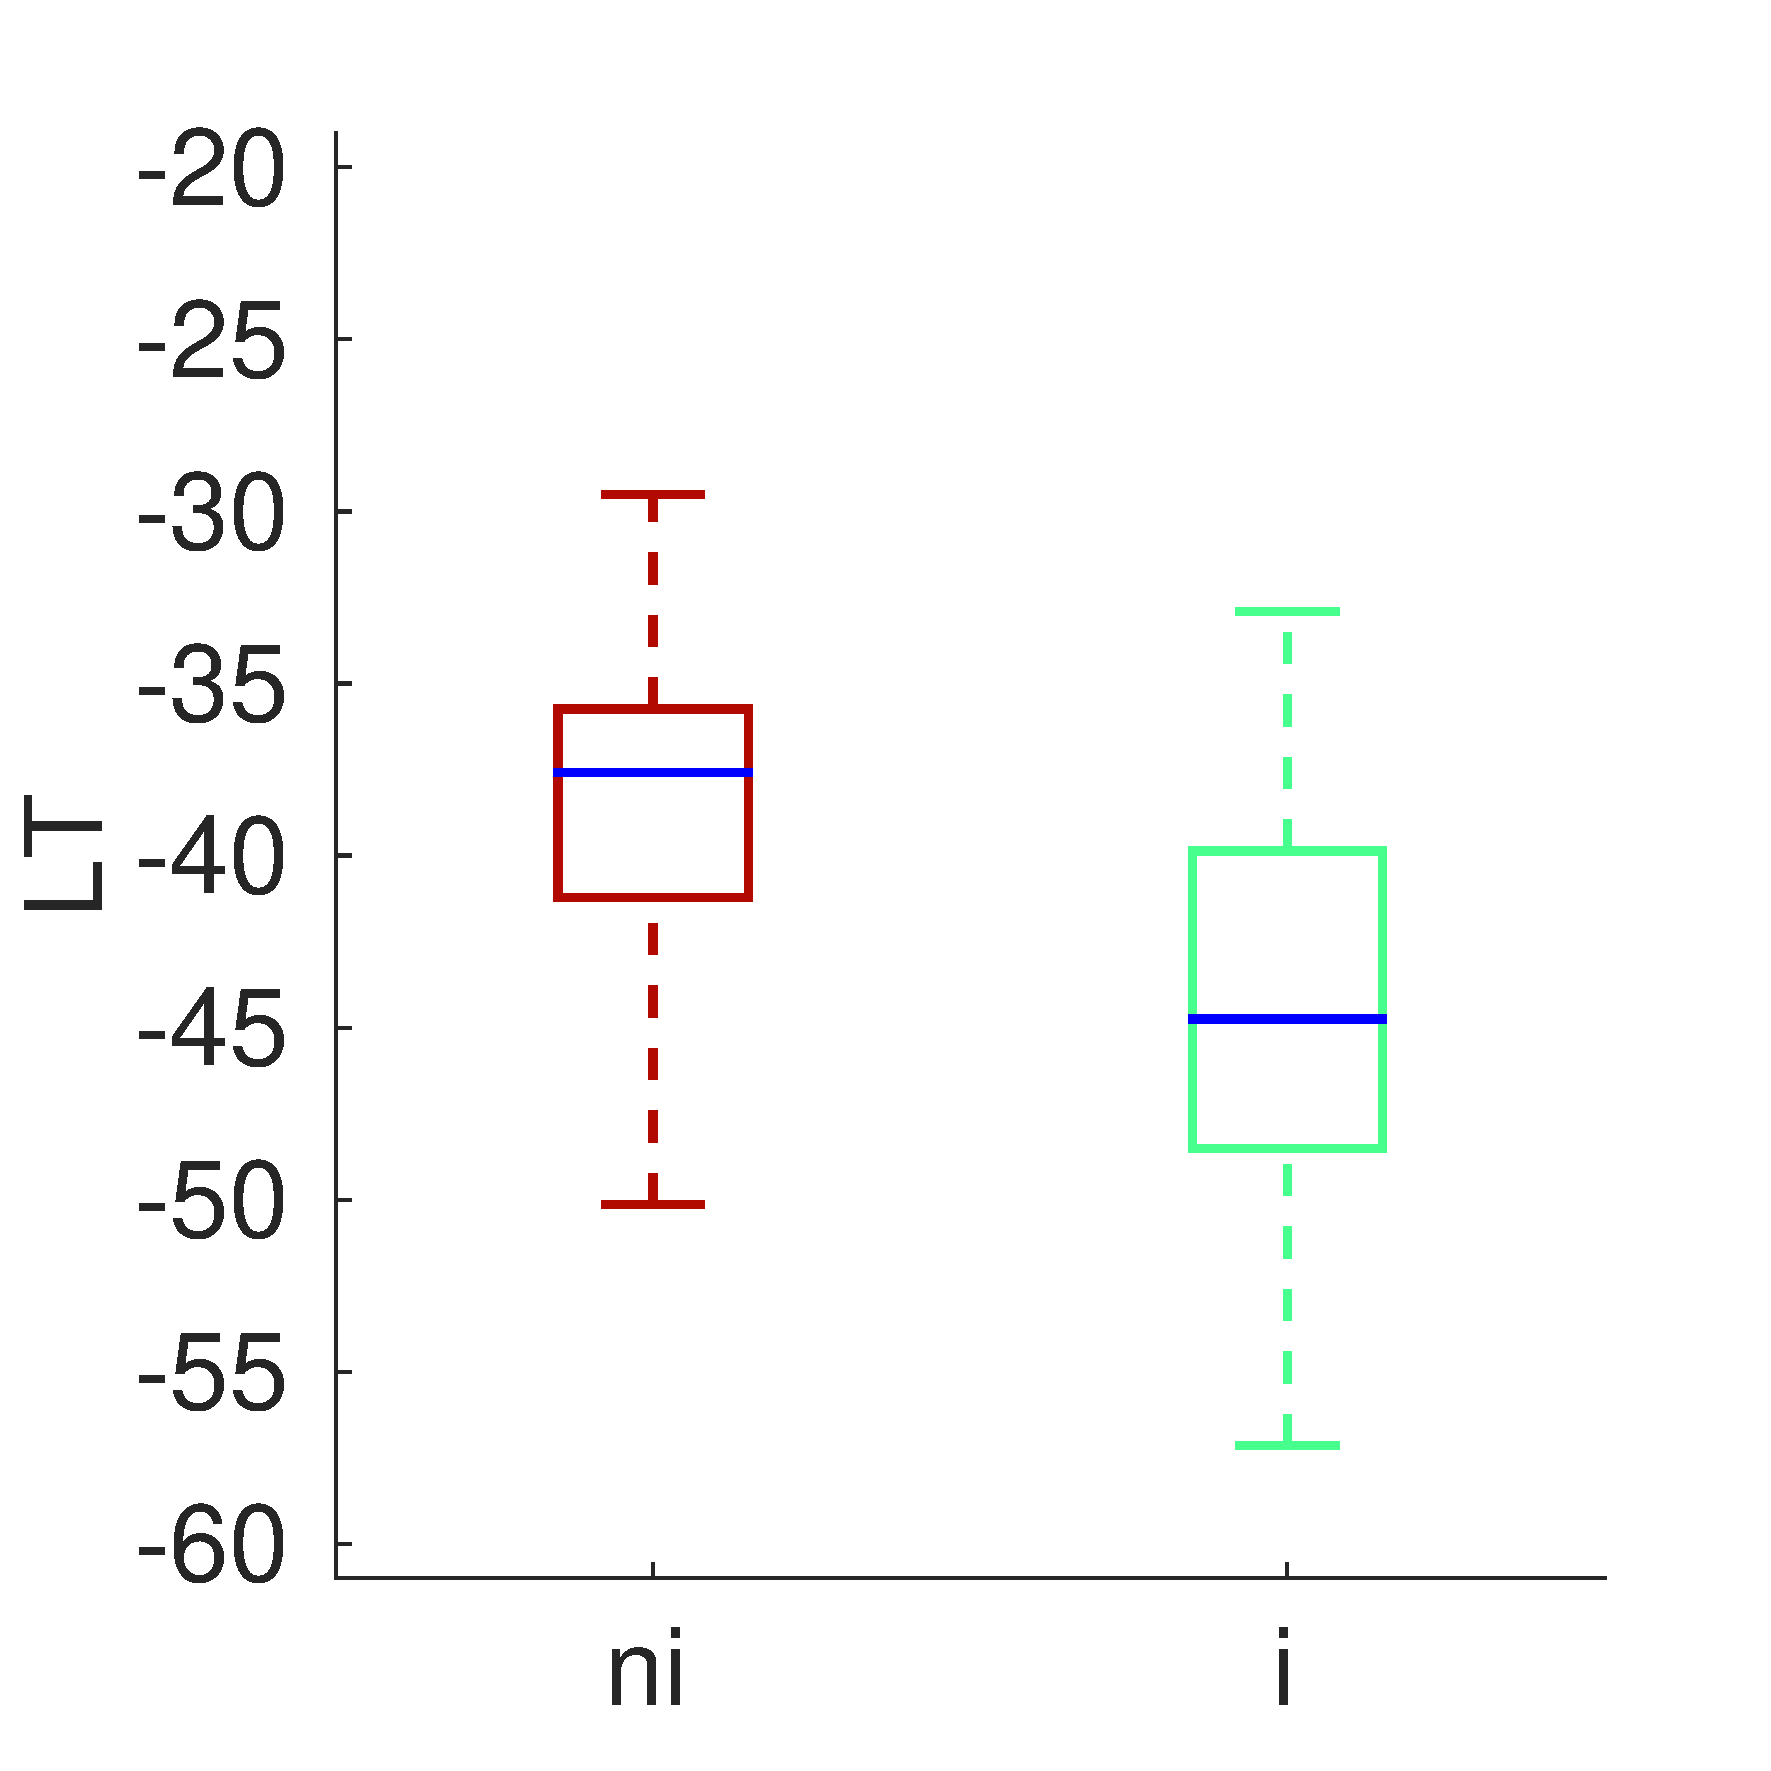
\includegraphics[width=.33\linewidth]{gfxXpUrbanSoundscape/xp_soundlevel_5}\label{fig:soundlevelc}}\par
        \subfloat[]
        {\includegraphics[width=.33\linewidth]{gfxXpUrbanSoundscape/xp_soundlevel_2}\label{fig:soundleveld}}
        \subfloat[]
        {\includegraphics[width=.33\linewidth]{gfxXpUrbanSoundscape/xp_soundlevel_4}\label{fig:soundlevele}}
        \subfloat[]
        {\includegraphics[width=.33\linewidth]{gfxXpUrbanSoundscape/xp_soundlevel_6}\label{fig:soundlevelf}}
       \caption[TODO]{TODO}\label{fig:soundlevel}
\end{figure}

\begin{figure}[t]
        \myfloatalign
        \subfloat[]
        {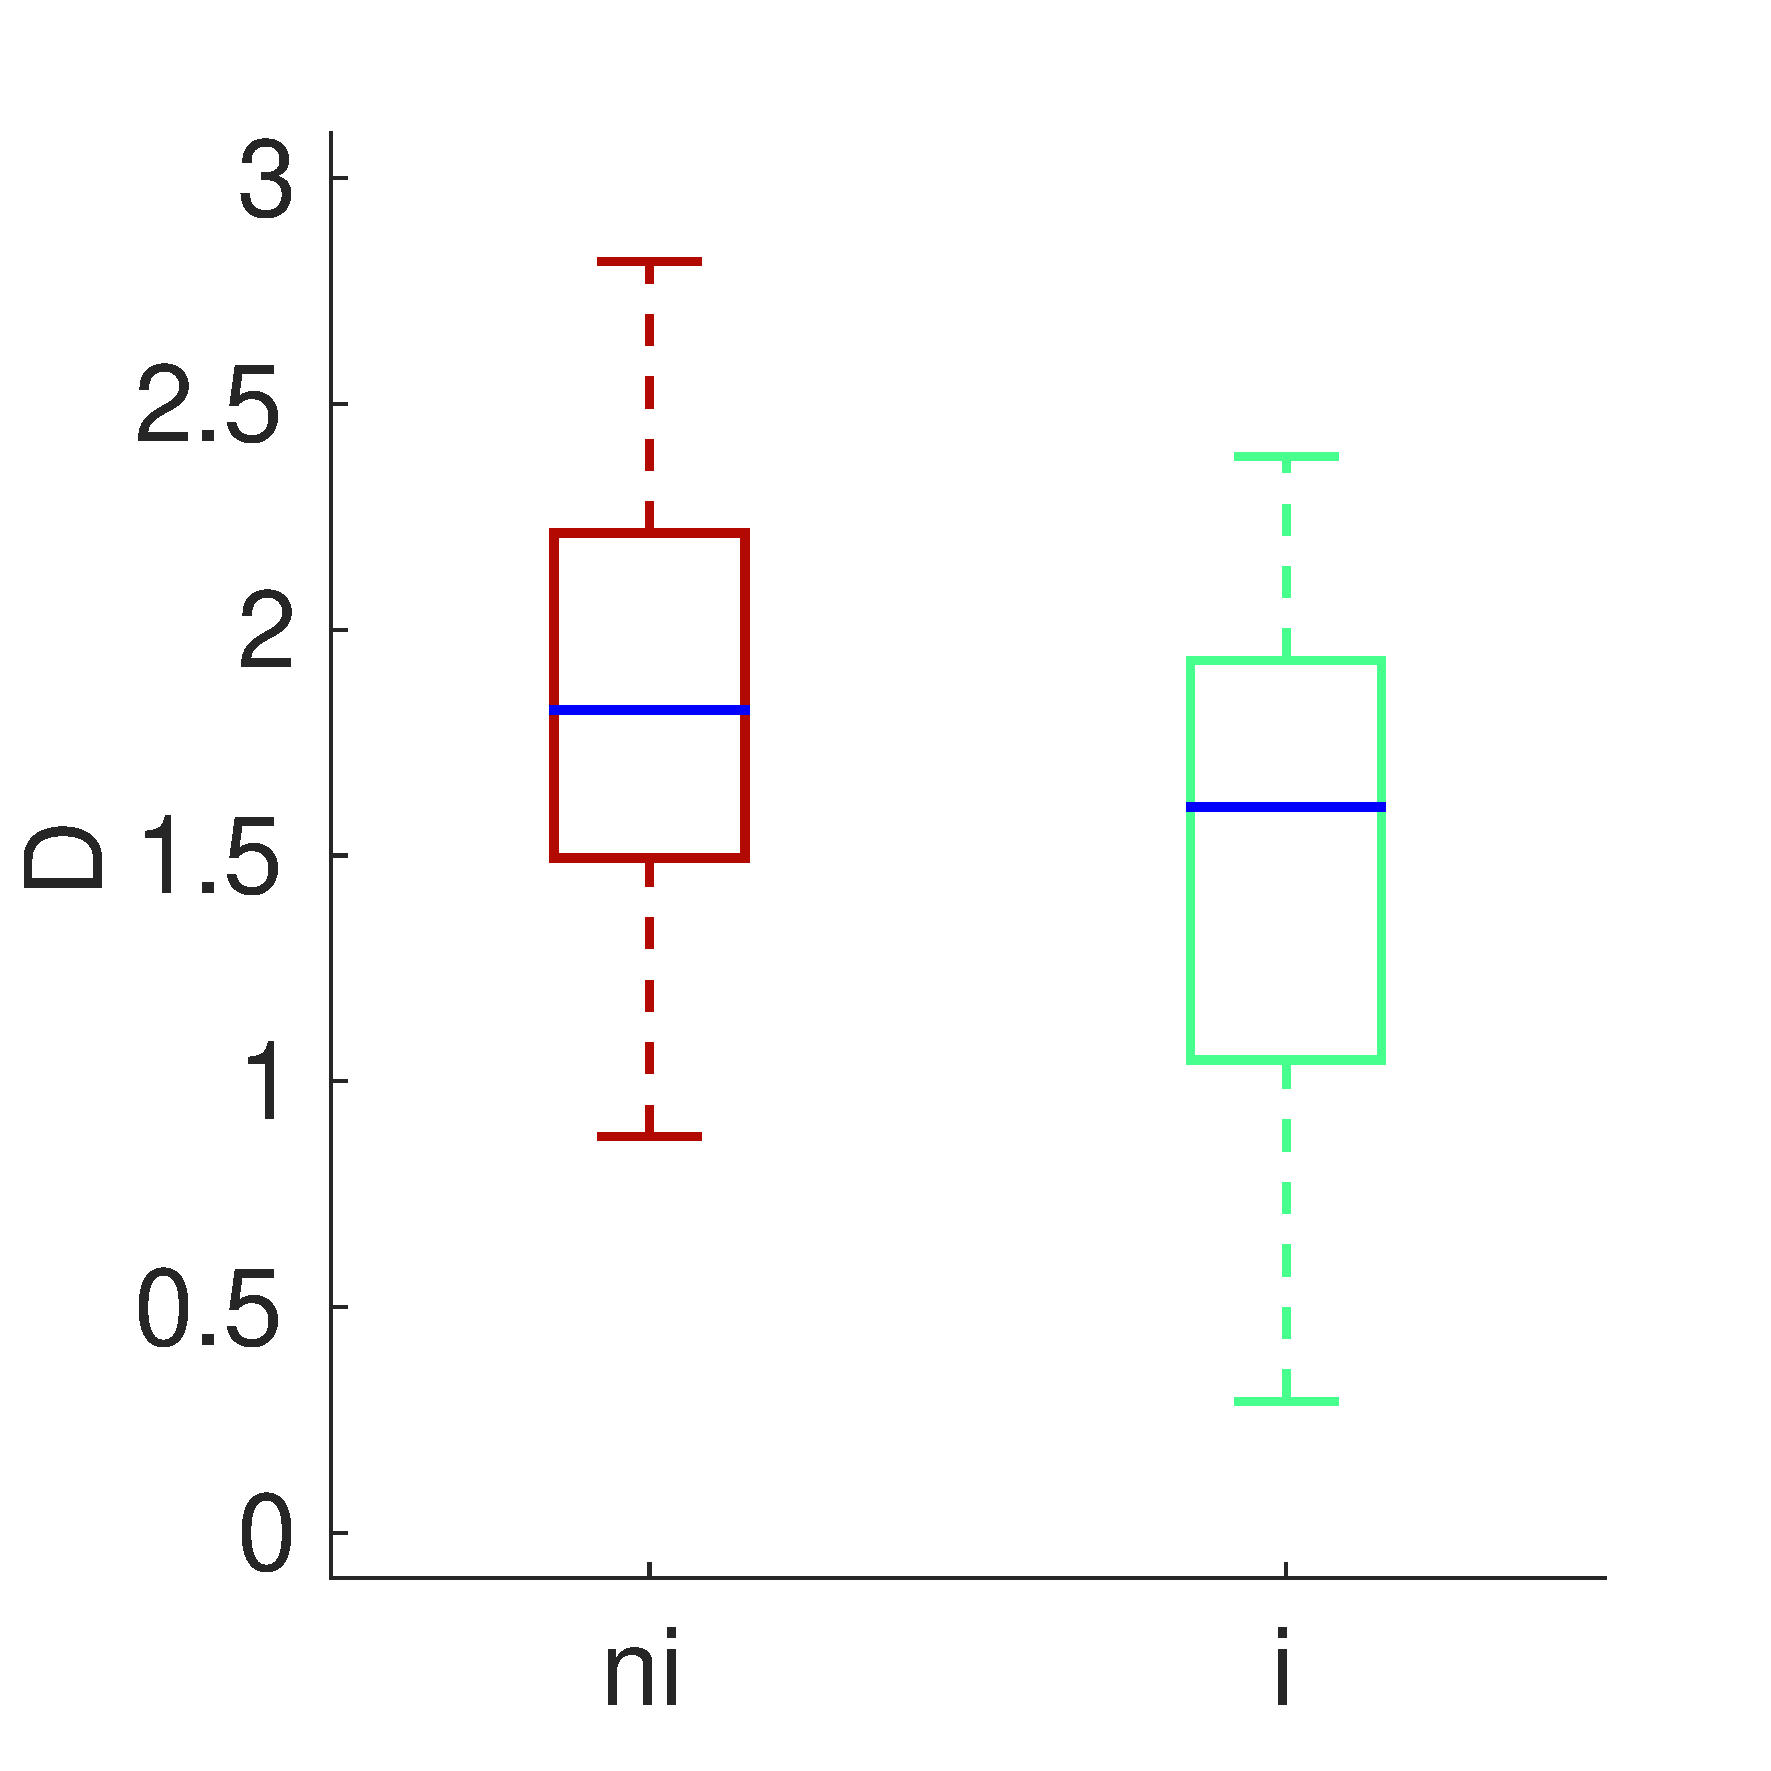
\includegraphics[width=.33\linewidth]{gfxXpUrbanSoundscape/xp_density_1}\label{fig:densitya}}
        \subfloat[]
        {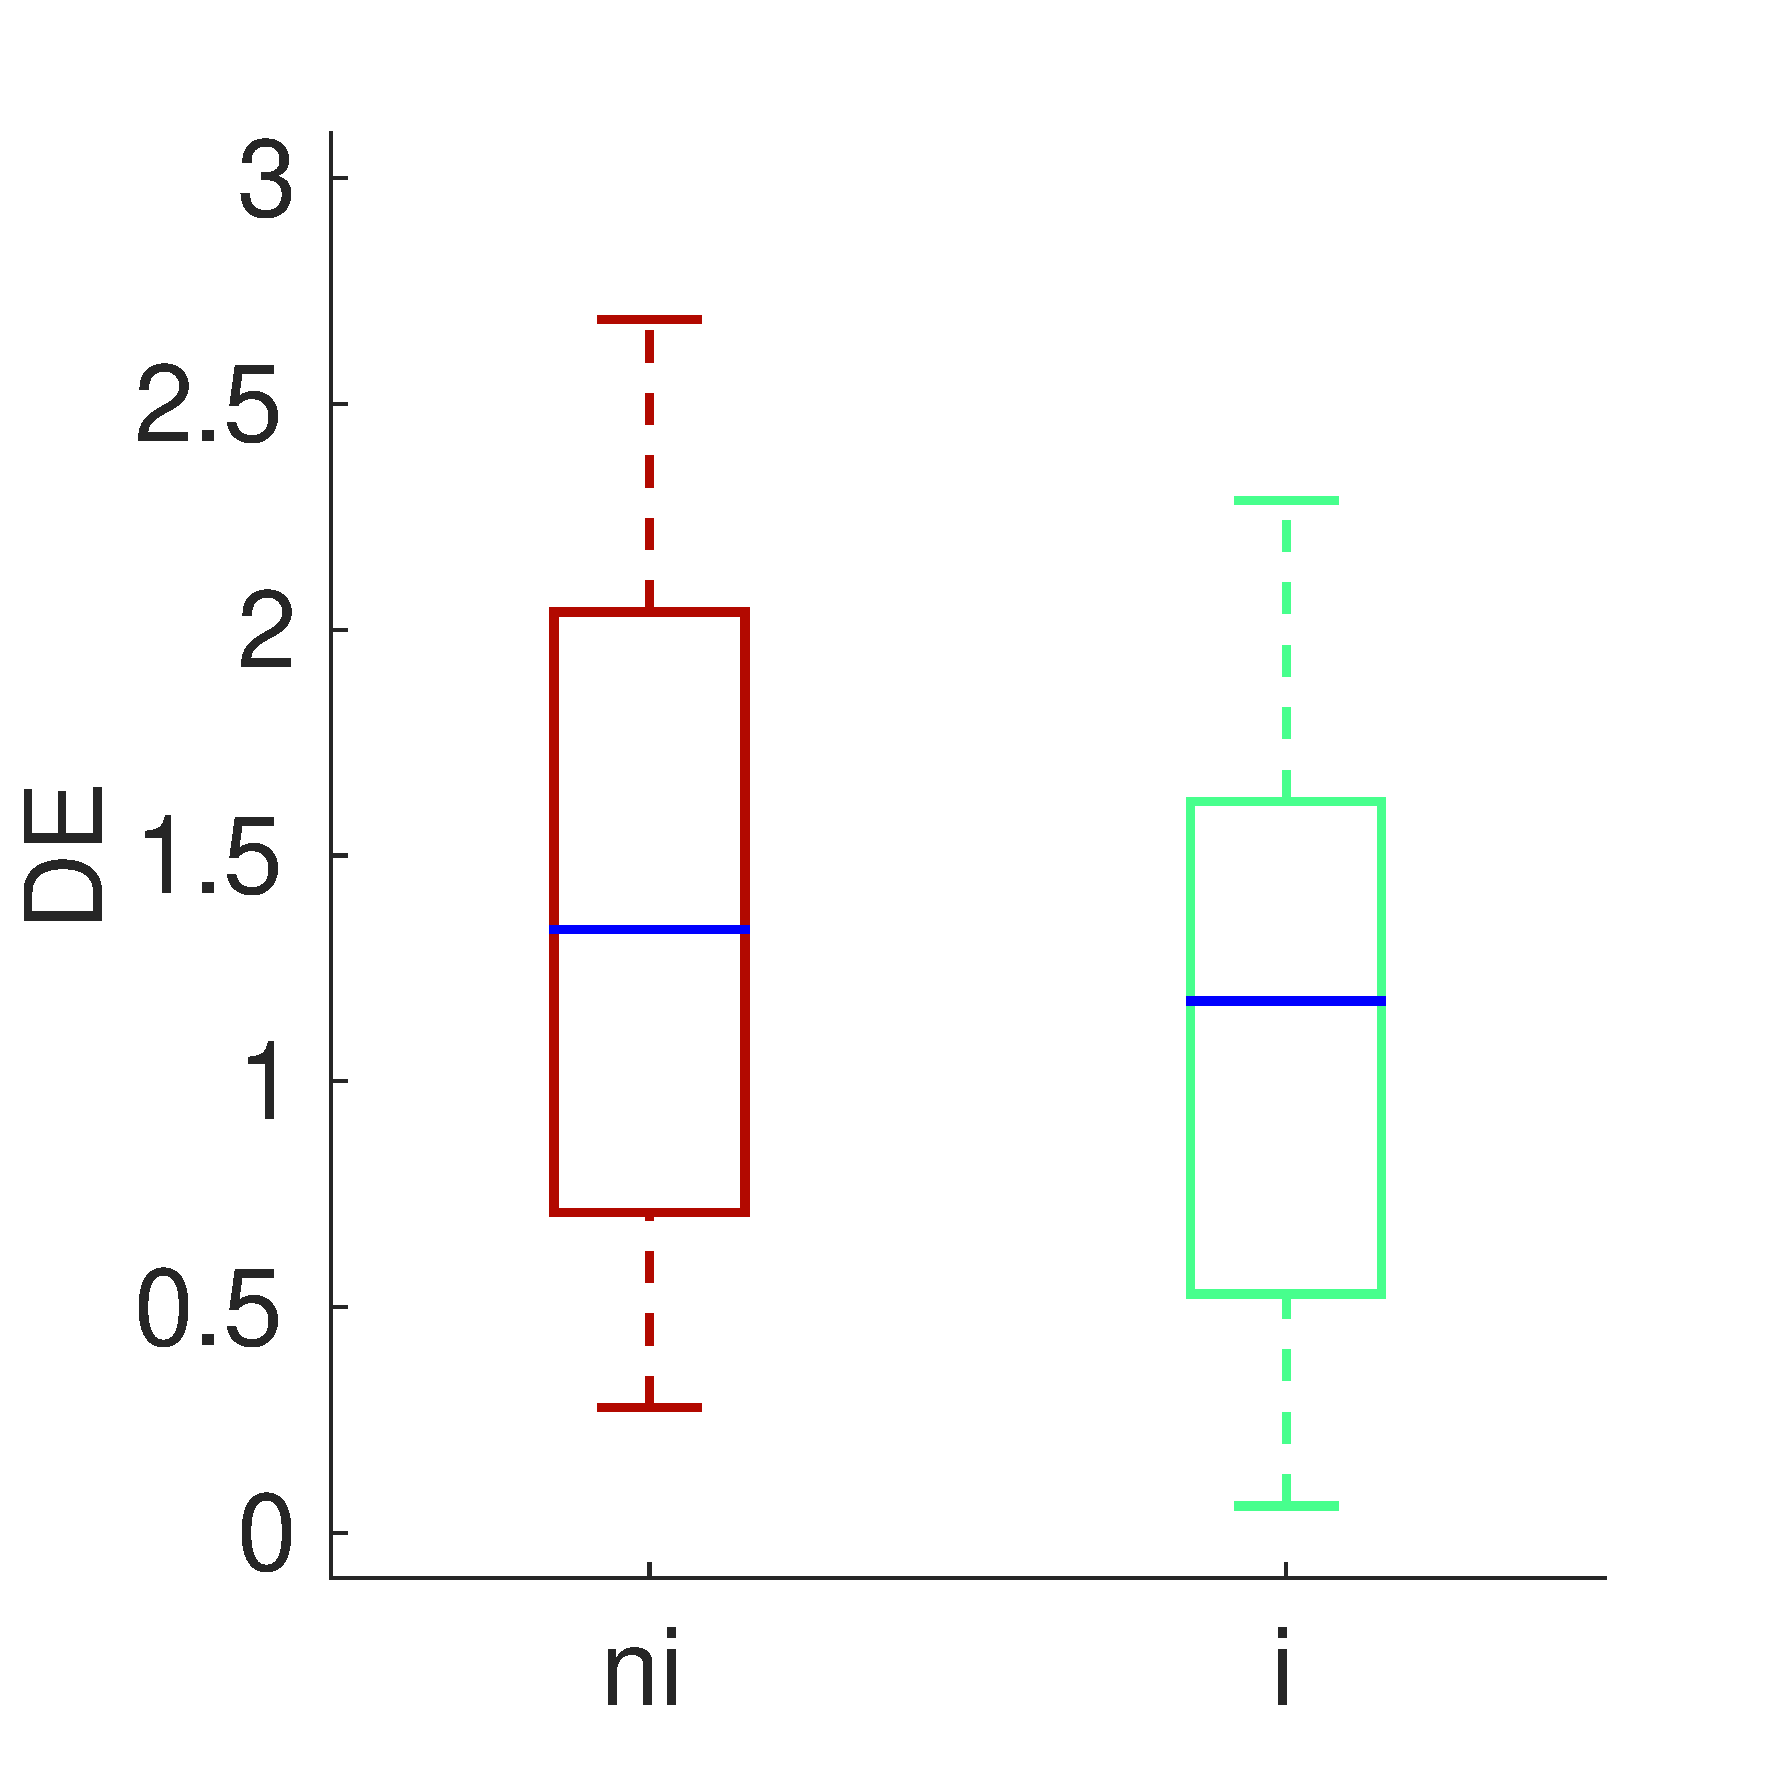
\includegraphics[width=.33\linewidth]{gfxXpUrbanSoundscape/xp_density_3}\label{fig:densityb}}\par
        \subfloat[]
        {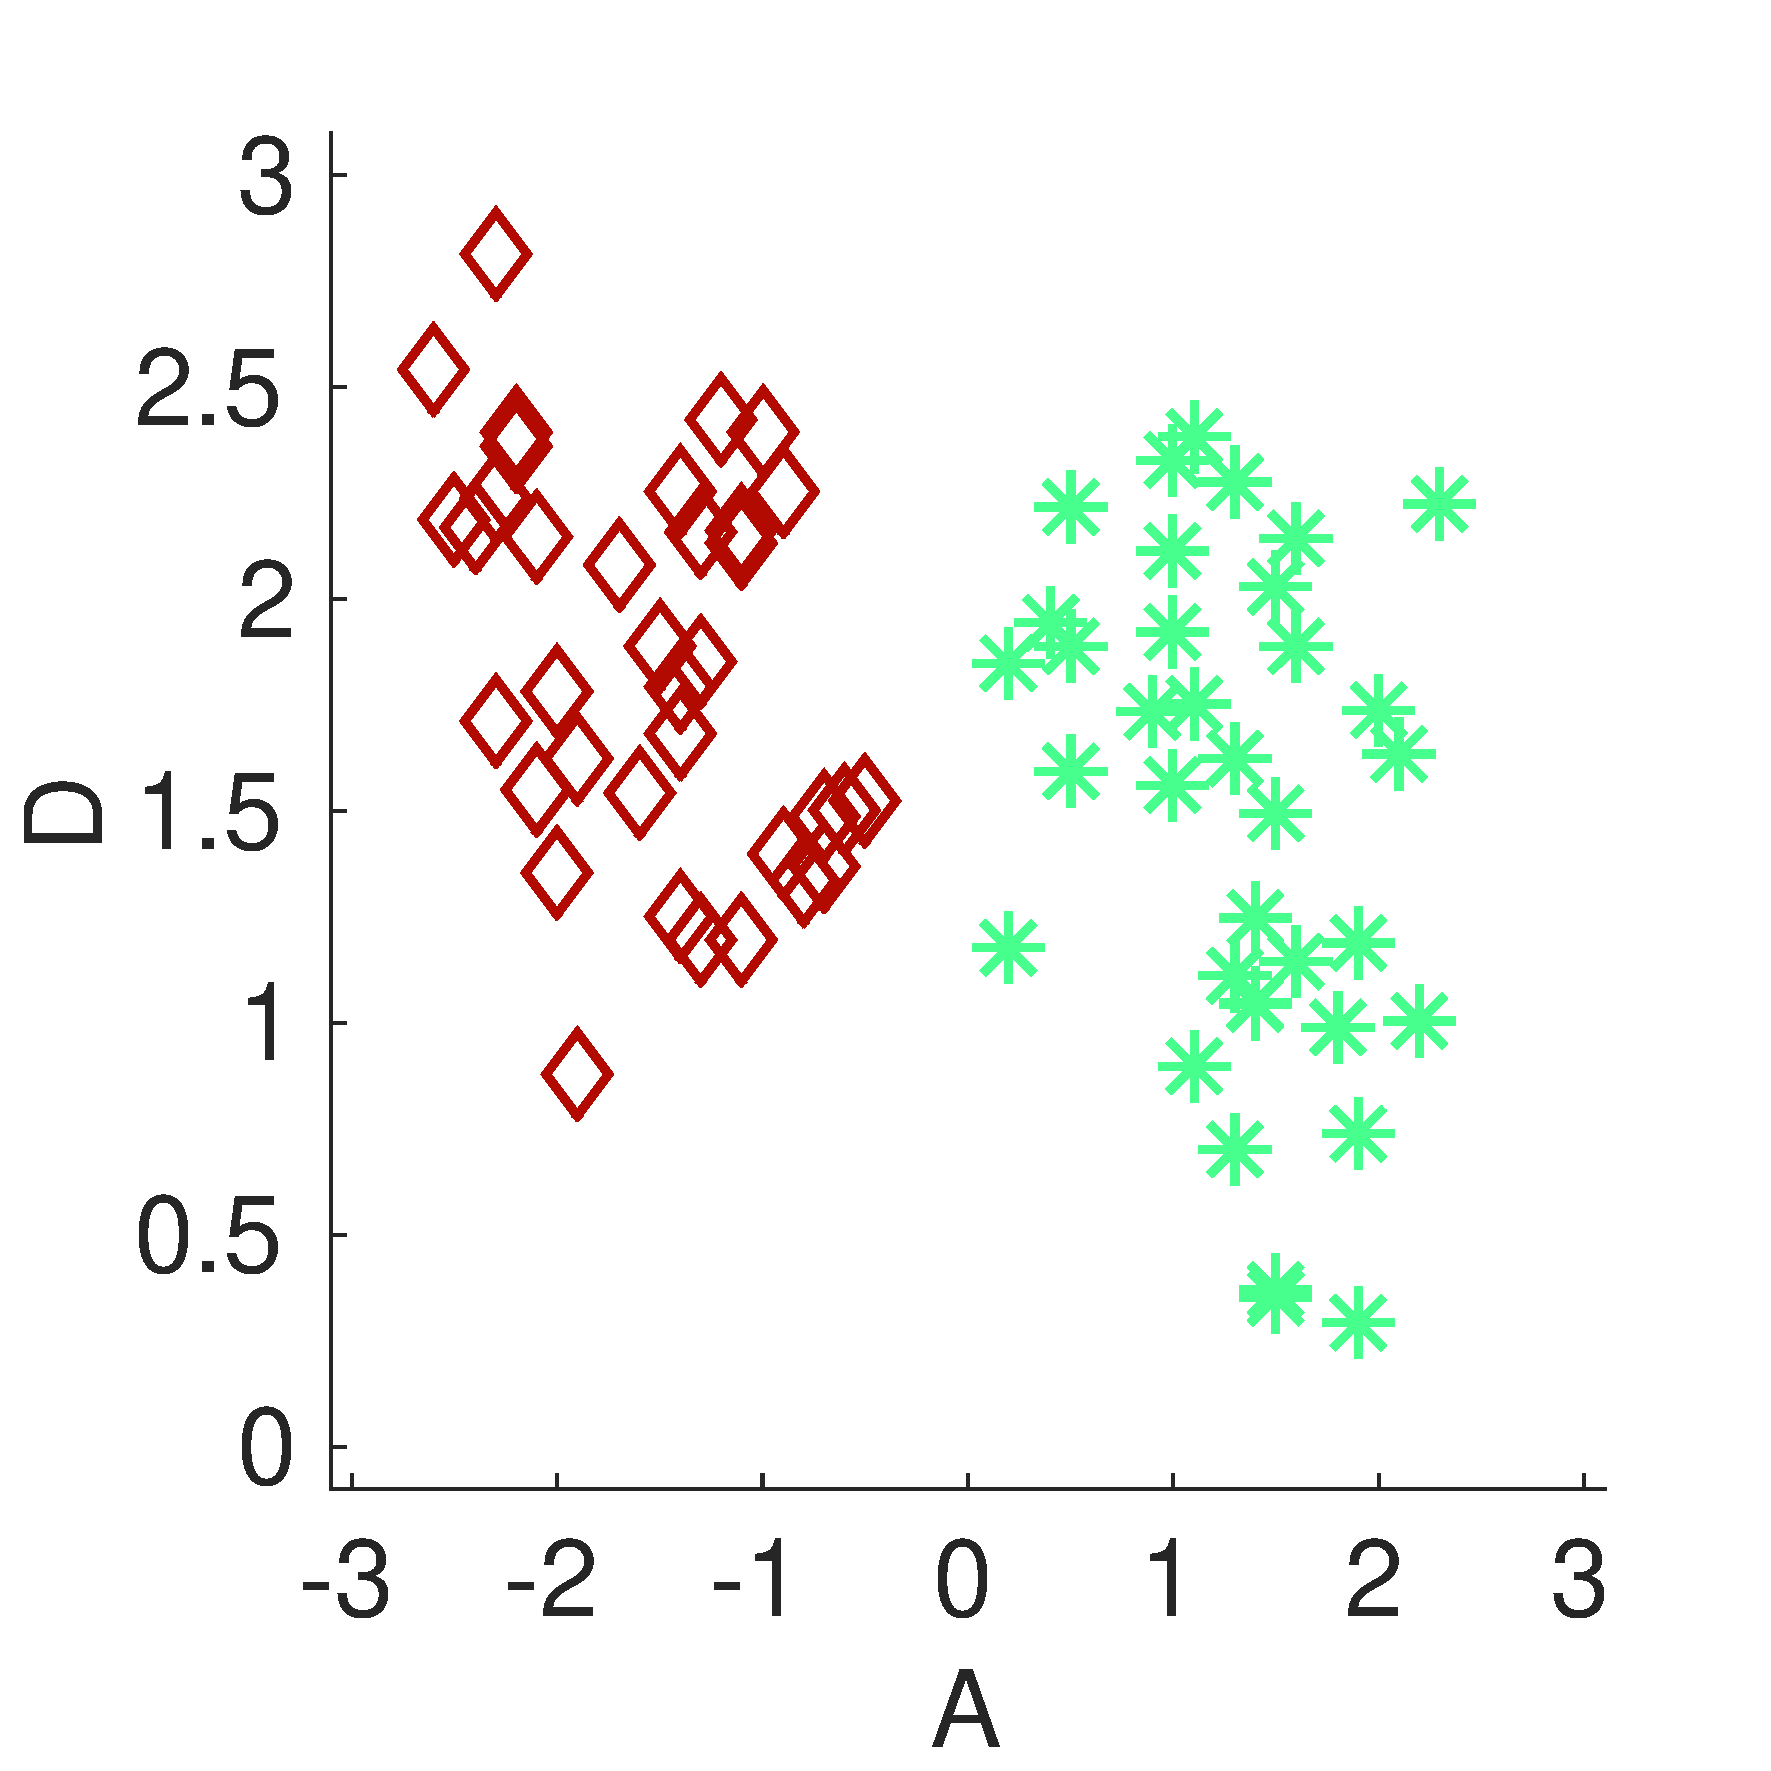
\includegraphics[width=.33\linewidth]{gfxXpUrbanSoundscape/xp_density_2}\label{fig:densityc}}
        \subfloat[]
        {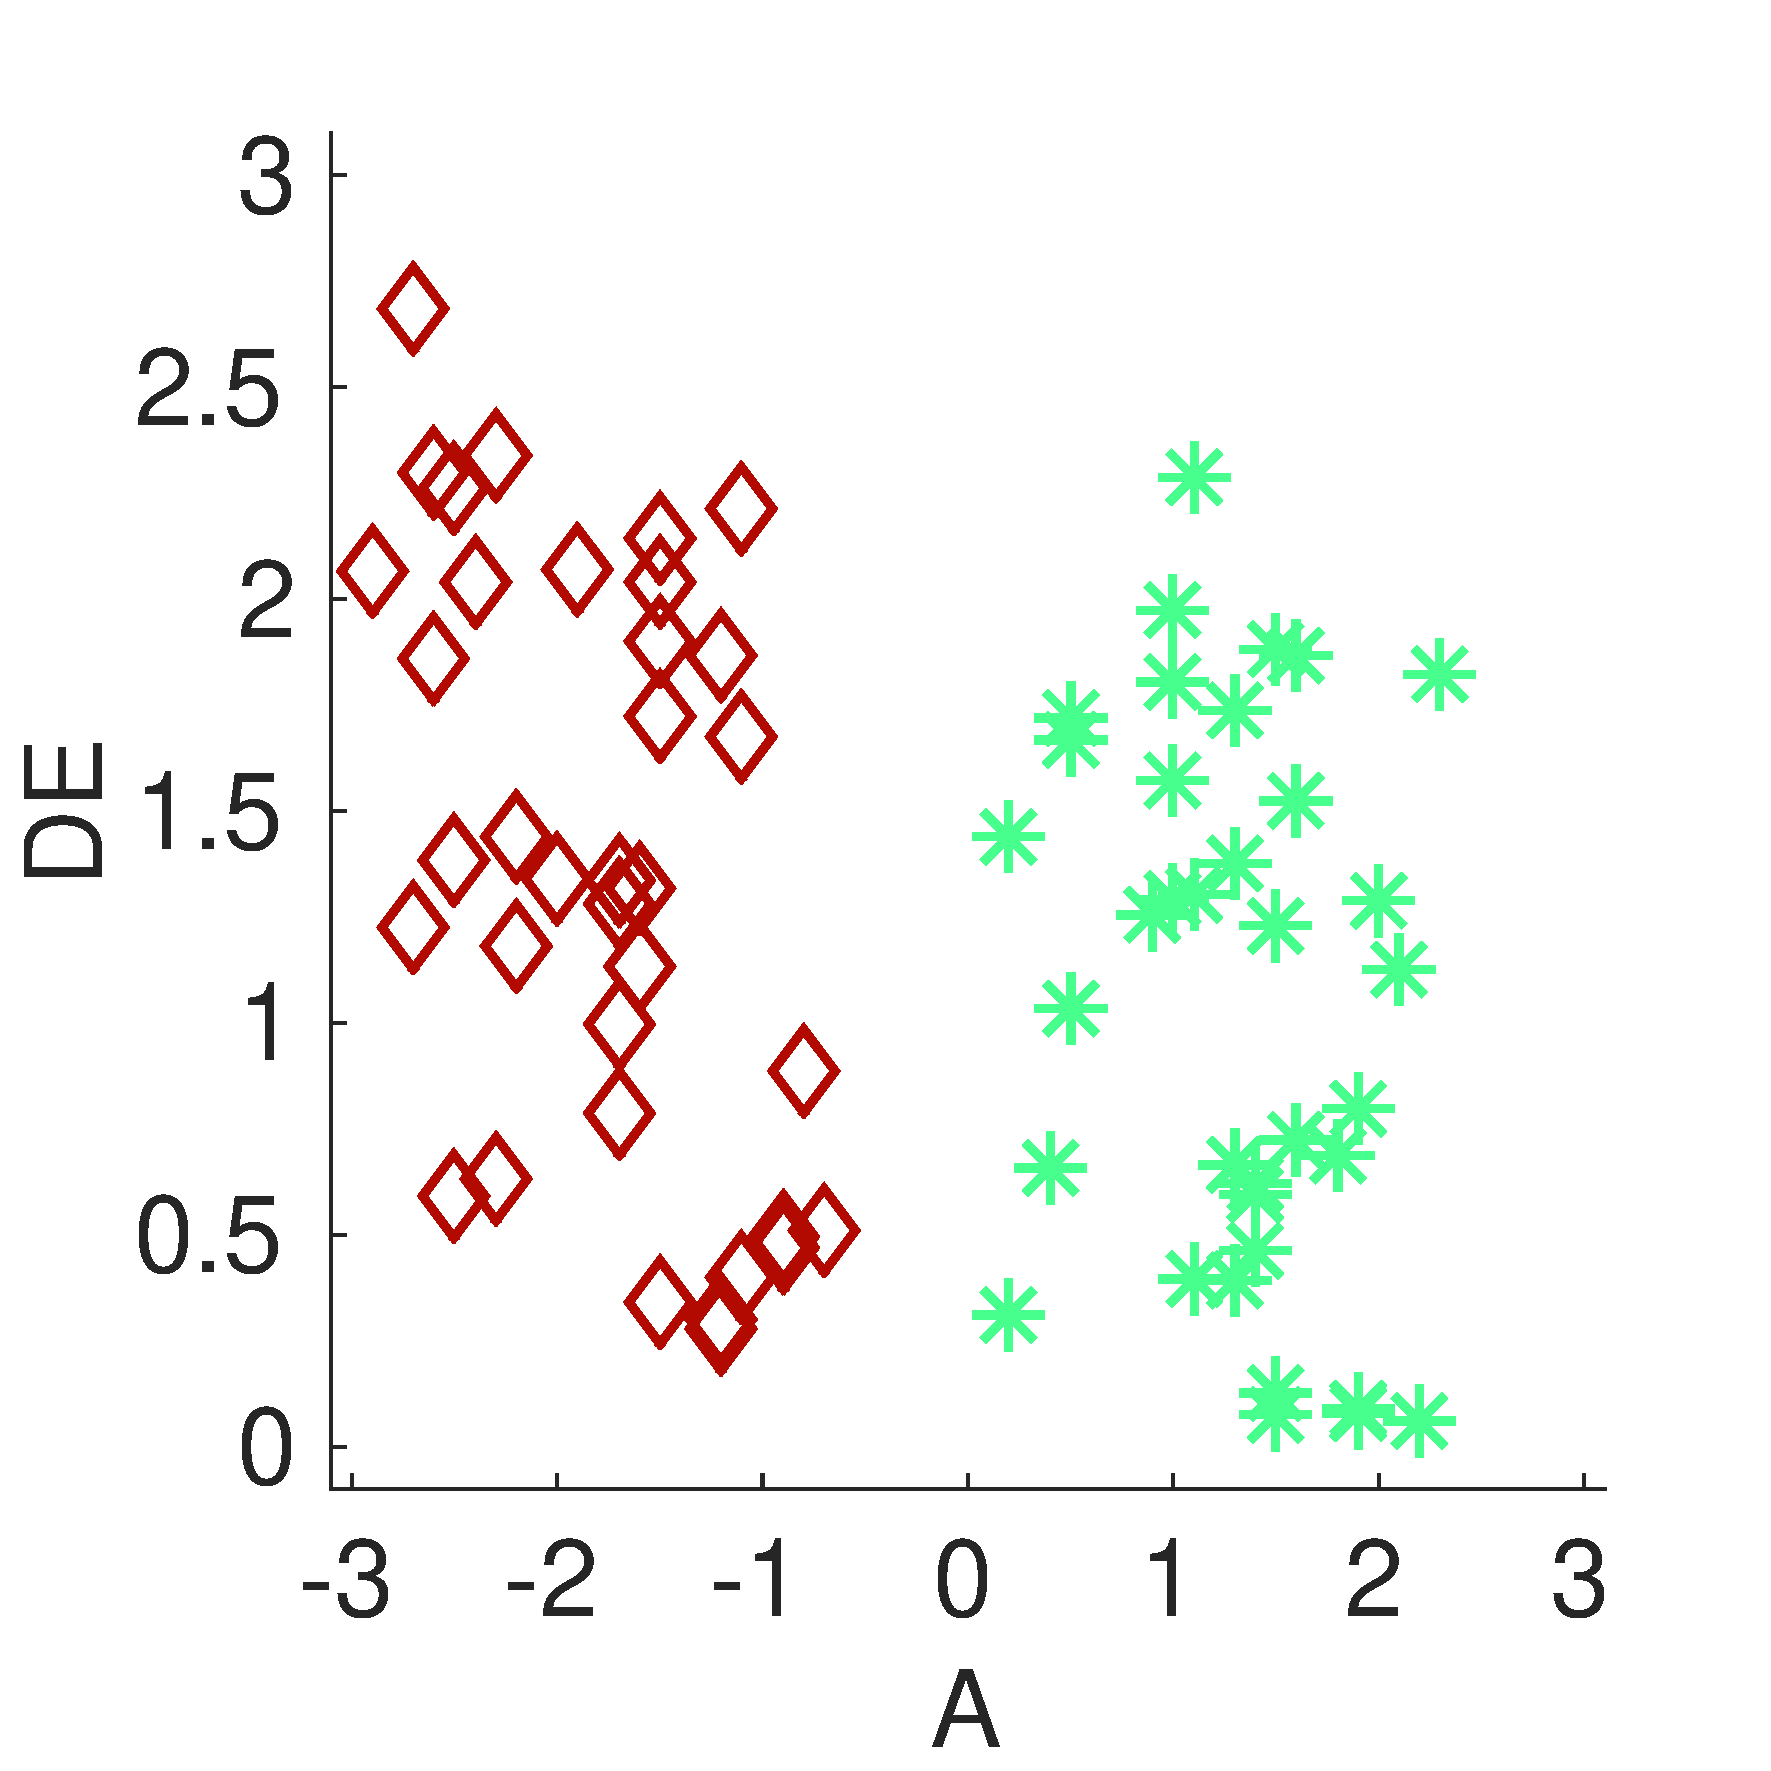
\includegraphics[width=.33\linewidth]{gfxXpUrbanSoundscape/xp_density_4}\label{fig:densityd}}
       \caption[TODO]{TODO}\label{fig:density}
\end{figure}

\begin{figure}[t]
        \myfloatalign
        \includegraphics[width=.9\linewidth]{gfxXpUrbanSoundscape/xp1_div_1}
       \caption[TODO]{TODO}\label{fig:diversity}
\end{figure}

\subsection{Influence des descripteurs structurels sur l'agrément perçu}
\label{sec:ch5_corrDesStruct}

Nous analysons, \jlc{exit:maintenant} dans cette section, les relations fines qui peuvent exister entre les descripteurs structurels d'une part et l'agrément perçu d'autre part. Contrairement à la section précédente, où la qualité affective des scènes est représentée de manière binaire (i \vs~ni), nous considérons, \jlv{dans cette section} \jls{ici}, l'agrément moyen $A$ comme descripteur perceptif. Il s'agit d'étudier l'existence de potentielles corrélations entre les descripteurs structurels et $A$. Les coefficients de corrélation linéaire calculés entre $A$ \vs~$L$, $L(E)$, $L(T)$, $D$, $D(E)$ et $DIV(E)$ sont présentés dans le tableau~\ref{tab:corrStructA}. Les relations entre $A$ et les descripteurs structurels sont illustrées par les figures~\ref{fig:soundleveld},~\ref{fig:soundlevele} et ~\ref{fig:soundlevelf} pour les niveaux sonores, et les figures~\ref{fig:densityc} et~\ref{fig:densityd} pour les densités. 

Concernant $L$, on observe une forte corrélation négative ($r=-0.76$, $p<0.01$) avec $A$, indiquant \jlc{exit:de fait} que plus le niveau sonore est élevé, plus la scène est désagréable. Cependant, la figure~\ref{fig:soundleveld} suggère que cette relation ne s'opère pas de la même manière pour les i- et ni-scènes. En effet, la corrélation entre $L$ et $A$ pour les ni-scènes reste élevée ($r=-0.67$, $p<0.01$), mais est inexistante pour les i-scènes. \jlv{Le fait que la corrélation entre $L$ et $A$, considérant l'ensemble des scènes, soit élevée, résulte du fait que les i-scènes ont tendance à être moins fortes que les ni-scènes, donnant ainsi l'illusion de prolonger la corrélation négative observée pour les ni-scènes} \jls{Cette corrélation élevée, quelles que soient les scènes, résulte du fait que les i-scènes ont tendance à être moins fortes que les ni-scènes, donnant ainsi l'illusion de prolonger la corrélation négative observée pour les ni-scènes}.  

On peut donc conclure que $L$:
\jls{Nous en concluons que $L$:}
\begin{itemize}
\item permet bien de faire la distinction entre les i- et ni-scènes,
\item permet de finement caractériser l'agrément perçu des ni-scènes,
\item n'est pas un indicateur pertinent de l'agrément perçu pour des environnements a priori agréables.
\end{itemize}

Les mêmes observations sont faîtes \jlv{si l'on considère} \jls{concernant} $L(E)$ (\cf~ref{fig:soundlevele}). \jlv{Pour les textures (\cf~ref{fig:soundlevelf}), bien que l'on observe une corrélation modérée si l'on considère l'ensemble des scènes ($r=-0.51$, $p<0.01$), aucune corrélation n'est relevée si l'on regarde séparément les i-scènes ($r=-0.33$, $p=0.05$) et les ni-scènes ($r=0.09$, $p=0.06$)} \jls{Pour les textures (\cf~ref{fig:soundlevelf}), bien que, à considérer l'ensemble des scènes, on observe une corrélation modérée, cela n'est pas vérifié quand on regarde séparément les i-scènes ($r=-0.33$, $p=0.05$) et les ni-scènes ($r=0.09$, $p=0.06$)}. Là encore \jlc{ce "Là encore" renvoie aux conclusions du passage précédent, où il est fait nulle mention d'une corrélation artificielle!!! il faut reformuler} on peut penser que la corrélation négative observée pour l'ensemble des scènes est artificielle, venant du fait que le niveau des textures des i-scènes a tendance à être plus bas que celui des ni-scènes. Ainsi, si les événements sonores conservent une certaine capacité de prédiction de l'agrément pour les ni-scènes, le niveau des textures n'apporte lui que peu d'informations, qu'importe l'environnement considéré \jls{quel que soit l'environnement}.

Considérant l'ensemble des scènes, nous observons une corrélation négative faible pour $D$ ($r=-0.41$, $p<0.01$) et $D(E)$ ($r=-0.34$, $p<0.01$). Là encore, une relation du même acabit est observée pour les ni-scènes, mais aucune corrélation n'est observée pour les i-scènes. La densité de sources sonores semble donc avoir un faible impact sur l'agrément perçu si l'on considère les ni-scènes, mais, comme pour les niveaux, la densité ne semble pas avoir d'impact pour les i-scènes.

En ce qui concerne la diversité des classes d'événements, une corrélation négative faible est obtenue pour les niveaux d'abstraction 1, 2 et 3 en tenant compte de l'ensemble des scènes. Si l'on considère les i- et ni-scènes séparément, aucune corrélation significative n'est trouvée. Les conclusions sont similaires à celles faites pour $L(T)$: la diversité permet uniquement de faire la distinction entre les deux types d'environnements, mais ne permet pas de caractériser précisément l'agrément perçu.

En résumer, en présence d'un environnement désagréable, les niveaux sonores, et en particulier ceux des événements, ainsi que, dans une moindre mesure, la densité de sources présentes, ont un impact négatif sur l'agrément. En présence d'un environnement agréable, aucun des descripteurs structurels considérés ici ne semble influer sur la perception de l'agrément. 

\jlv{Ces premiers résultats tendent à suggérer qu'il existerait deux modes de perceptions, engageant chacun des descripteurs indépendants, et qui s'activeraient en fonction de la nature de l'environnement en présence (i ou ni).} 
\jls{Ces premiers résultats pourraient montrer qu'il existe deux modes de perception, mobilisant chacun des descripteurs indépendants, modes qui s'activent en fonction de la nature de l'environnement en présence (i ou ni).} 

Le fait qu'aucun des descripteurs globaux ne permettent de caractériser l'agrément des i-scènes peut nous amener à penser que toutes les sources sonores ne contribuent pas de manière égale à la perception de l'agrément, mais, que seules les caractéristiques de certaines d'entre elles ont une réelle influence. Afin approfondir ce point, nous analysons, dans la section suivante, les scènes d'un point de vue sémantique, \ie~en nous intéressant à la nature des sources qui les composent. \\

\gl{Ici discussion et convergence avec d'autres papiers}

\begin{table}[t]
\centering
\begin{tabular}{l c c c} 
            & ensemble                     & i-scènes                   & ni-scènes    \\
\hline
$L$         & \textbf{-0.76} ($p<0.01$)    & -0.32 ($p=0.06$)           & \textbf{-0.67} ($p<0.01$)\\
$L(E)$        & \textbf{-0.75} ($p<0.01$)    & -0.20 ($p=0.24$)           & \textbf{-0.75} ($p<0.01$)\\
$L(T)$        & \textbf{-0.51} ($p<0.01$)    & -0.33 ($p=0.05$)           &  0.09  ($p=0.6$) \\
$D$         & \textbf{-0.41} ($p<0.01$)    & -0.31 ($p=0.07$)           & \textbf{-0.37} ($p=0.03$)\\
$D(E)$        & \textbf{-0.34} ($p<0.01$)    & -0.22 ($p=0.21$)           & \textbf{-0.47} ($p<0.01$)\\
$DIV(E)$ 0     &          -0.07 ($p=0.57$)    & -0.25 ($p=0.15$)           & -0.22 ($p=0.23$)\\
$DIV(E)$ 1     & \textbf{-0.46} ($p<0.01$)    & -0.25 ($p=0.14$)           & -0.18 ($p=0.30$)\\
$DIV(E)$ 2     & \textbf{-0.40} ($p<0.01$)    & -0.21 ($p=0.22$)           & -0.18 ($p=0.30$)\\
$DIV(E)$ 3     & \textbf{-0.36} ($p<0.01$)    & -0.18 ($p=0.30$)           & -0.18 ($p=0.30$)\\
\hline
\end{tabular}
\vspace{0.5mm}
\caption{Coefficients de corrélation linéaire calculés entre l'agrément perçu moyen $A$ \vs~TODO}
\label{tab:corrStructA}
\end{table}

\subsection{Étude comparative entre les descripteurs sémantiques}

\subsubsection{Analyse qualitative}

Nous analysons la composition des scènes en comptant le nombre de sujets ayant utilisé une classe de sons pour simuler un type d'environnements. Les résultats sont présentés à la figure~\ref{fig:soundsourcea} pour les événements et à la figure~\ref{fig:soundsourceb} pour les textures. Par souci d'espace, nous choisissons un niveau d'abstraction intermédiaire entre le niveau 0 et 1, noté $0+$, pour représenter les classes (\cf~Figure~\ref{fig:taxonomie}).

Nous observons une différence notable dans le choix des classes entre les i- et ni-scènes. La répartition des classes est très proche de celles obtenues dans une étude similaire sur les environnements sonores urbains idéales \jlc{idéaux} \citep{guastavino2006ideal}, \ie~les classes suggérant la présence humaine et la nature sont très présentes dans les i-scènes, a contrario les classes désignant des sons mécaniques et de travaux sont principalement utilisées pour les ni-scènes.

Ces résultats confirment un fait déjà observé, la nature sémantique des sources sonores joue un rôle prédominant dans l'appréciation de l'environnement \citep{raimbault2005urban,dubois2006cognitive}.

Nous notons quelques différences avec \citep{guastavino2006ideal}: les résultats obtenus par Guastavino~\al montrent que les sons de \emph{transports publics} sont caractéristiques des environnements sonores urbains idéales \jlc{idéaux}. Les auteurs attribuent ce fait que \jlc{cela au fait que} la perception de l'agrément est, entre autre, soumise à un contexte socio-culturel. Dans notre représentation du monde, les sons de transports publics sont positivement connotés, et ont ainsi tendance à être mieux acceptés que les sons de véhicules privés.

Dans une certaine mesure, nos résultats contredisent ce fait. La figure~\ref{fig:soundsourcea}  montre, en effet, que les classes d'événements de \emph{transports publics} (\emph{bus} et \emph{train}, \cf~Figure~ref{fig:soundsourcec}) ont été utilisées par $28\%$ des sujets pour les i-scènes, mais également  par $42\%$ des sujets pour les ni-scènes \jls{ont été utilisées par les sujets, pour des i-scènes, dans $28\%$ des cas, et pour des ni-scènes, dans $42\%$ des cas}. Les résultats ne renient pas \jls{ne remettent pas en question} le fait que  les sons de \emph{transports publics} soient bien acceptés: $25\%$ des sujets ont utilisés la classe \emph{bus} pour les i-scènes, \jlv{soit autant que la classe \emph{Vélo}, et plus qu'aucune autre classe de véhicules privés} \jls{un chiffre comparable à celui de la classe \emph{Vélo}, et bien supérieur à celui de toute autre classe de véhicules privés}. Cependant les classes \emph{transports publics} sont également bien présentes dans les ni-scènes, plus que les classes \emph{voiture} ou \emph{camion} par exemple. De ce fait, la classe \emph{transports publics} ne peut être considérée \jls{La classe \emph{transports publics} ne peut donc pas être considérée} comme typique d'un environnement sonore urbain idéal.

Cette différence peut s'expliquer par la nature des deux protocoles expérimentaux utilisés. \jlv{Comme pour notre épreuve de simulation, Guastavino~\al demande aux sujets de décrire un environnement en se basant sur leurs mémoires. Cependant, contrairement à nous, les sujets de Guastavino~\al ne disposent pas de supports sonores} \jls{Comme nous l'avons fait, Guastavino~\al demande à ses sujets de décrire un environnement en se basant sur leurs mémoires. Mais, contrairement à nous, les sujets de Guastavino~\al ne disposent pas de supports sonores}. Le fait que nos sujets soient confrontés à la réalité acoustique des sons pour recréer leurs environnements peut avoir pour effet de diminuer l'effet du contexte socio-culturel. D'autres études utilisant des sons comme stimuli montrent que la classe \emph{bus} peut avoir un effet négatif sur l'appréciation de l'environnement \citep{lavandier2006contribution}.

\begin{figure}[t]
        \myfloatalign
        \subfloat[]
        {\includegraphics[width=.8\linewidth]{gfxXpUrbanSoundscape/xp1_class_1}\label{fig:soundsourcea}} \par
        \subfloat[]
        {\includegraphics[width=.4\linewidth]{gfxXpUrbanSoundscape/xp1_class_2}\label{fig:soundsourceb}} 
        \subfloat[]
        {\includegraphics[width=.4\linewidth]{gfxXpUrbanSoundscape/xp1_class_3}\label{fig:soundsourcec}} 
       \caption[TODO]{TODO}\label{fig:soundsource}
\end{figure}

\subsubsection{Marqueurs sonores}

\jlv{Nous venons de voir qualitativement que la composition} \jlc{ce "qualitativement" est mal placé, et puis, es-tu sûr de vouloir l'utiliser ?} des sources sonores des scènes semble différer entre les deux types d'environnements (i et ni) \jls{Nous avons mis en évidence que, qualitativement, la composition des sources sonores des scènes diffère selon les types d'environnements (i ou ni)}. Nous essayons de voir maintenant si, parmi ces classes, certaines, appelées marqueurs sonores, sont typiques d'un environnement en particulier. Pour ce faire, nous utilisons le V-test (\cf~section~\ref{sec:ch5_methodoEtStat}), en considérant séparément chaque niveau d'abstraction. Les résultats sont présentés dans le tableau~\ref{tab:markers}.

Concernant les événements sonores, 9 marqueurs sont identifiés sur l'ensemble des niveaux d'abstraction. Comme la figure~\ref{fig:soundsource} nous le laissait présager, les classes relatives à l'activité humaine (\emph{pas homme béton},\emph{sonnette vélo}), et à la nature (\emph{animaux, oiseaux},\emph{chants d'oiseaux}) sont des marqueurs de i-scènes. Nous notons également la présence de la classe \emph{cloche} dans les marqueurs d'un environnement idéal. Ce fait \jlv{peut être attribué} \jls{Ce fait est possiblement dû} au background socio-culturel des sujets, dans leur grande majorité des citoyens européens. En effet, selon Schafer, un son reconnu par un individu comme faisant partie intégrante de son environnement est bien accepté. Les marqueurs de ni-scènes sont des classes faisant référence à des sons de travaux (\emph{travaux}), ou suggérant un trafic dense (\emph{klaxon}, \emph{sirène}). \jlc{exit:"Bien que les marqueurs des ni-scènes soient intuitifs". la phrase est reprise plus bas}.

Concernant les textures sonores, 5 marqueurs sont identifiés. Pour les i-scènes, il s'agit de classes faisant référence à des ambiances amorphes, calmes, (\emph{cour-intérieur/parc} et \emph{parc}). Pour les ni-scènes, il s'agit, comme pour les événements, de classes faisant référence à des bruits de travaux (\emph{travaux} et \emph{véhicule de travaux}), ainsi que d'une classe faisant référence au trafic (\emph{carrefour}).


\jlv{Bien que l'ensemble des marqueurs identifiés soient intuitifs, nous notons qu'aucune des classes d'événements faisant directement référence aux bruits de véhicules motorisés n'en fait partie. Seule une classe marqueur de texture y fait référence (\emph{carrefour})} \jls{Bien que l'ensemble des marqueurs identifiés soient intuitifs, nous notons aucune des classes d'événements faisant directement référence aux bruits de véhicules motorisés dans leur nombre, exception faite du marqueur de texture (\emph{carrefour})}. Pour représenter un trafic désagréable, les sujets ont porté leur choix sur les classes \emph{klaxon} et \emph{sirène}. On peut supposer que les sons isolés de véhicules sont compris comme faisant partie intégrante de l'environnement urbain, et ne sont ainsi pas particulièrement associés à un environnement désagréable. \\ 

\gl{ici analyse des caractéristiques des classes trafics}
 
\begin{table}[t]
 \setlength{\tabcolsep}{0.2pt}
 \centering
  {\renewcommand{\arraystretch}{0.9}
\begin{tabular}{c c c c} 
Niveau        & \multicolumn{2}{c}{Marqueurs sonores événements} \\
d'abstraction & i-scènes & ni-scènes \\
\hline
0  &                               &  construction work (3.78)  \\
\hline
  & church bell  (4.5)             & horn  (3.9) \\
1 & bell bike    (4.3)             & siren (3.9)\\
  & animal       (4.2)             &       \\
   \hline
  & birds        (4.8)             & horn  (4.0)\\
2 & church bell  (4.4)             & siren (4.0)\\
  & bell bike    (4.2)             &       \\
   \hline
  & birds singing (4.8)            & horn  (4.1)\\
  & church bell   (4.3)            & siren (4.0)\\
3 & bell bike     (4.2)            &       \\
  & male footsteps                 &  \\
  &   concrete (3.6)               &  \\
  \hline
  \hline
          & \multicolumn{2}{c}{Marqueurs sonores textures}      \\
\hline
0         &     courtyard/park (4.1) &  construction work (3.9)  \\
\hline
          &     park (3.65)           &  crossroads (3.6)  \\
1         &     park (3.65)           &  vehicle work (3.3)  \\
\hline
2         &     park (3.64)           &  crossroads (3.56)  \\
\end{tabular}
}
\vspace{0.5mm}
\caption[Classes d'événements identifiées \jlc{identifiées se rapporte bien à classes ?} comme étant des marqueurs sonores]{Classes d'événements identifiées comme étant des marqueurs sonores. Dans chaque cellule, les marqueurs sont ordonnés par ordre décroissant de valeur $V$.}
\label{tab:markers}
\end{table}

\subsection{Étude des espaces de représentations induits par les descripteurs sémantiques}

Dans cette partie, nous évaluons la capacité d'une représentation sémantique à séparer les deux types d'environnements. Pour ce faire, nous calculons une précision au rang 5 ($p@5$) sur l'espace induit par les descripteurs sémantiques $S$, et ce pour chaque niveau d'abstraction (\cf~section~\ref{sec:ch5_methodoEtStat}). Les vecteurs $S$ sont construits en utilisant toutes les classes ($ET$), les classes d'événements ($E$), les classes de textures ($T$), \jlv{les classes d'événements en ne considérant que les marqueurs sonores ($E_m$)} \jls{les classes d'événements ne considérant que les marqueurs sonores ($E_m$)}, \jlv{les classes d'événements sans considérer les marqueurs sonores ($E_{w/o,m}$)} \jls{les classes d'événements ne considérant pas les marqueurs sonores} \jlc{je ne suis pas sûr que cette dernière suggestion soit pertinente. Ca dépend de l'acceptation des mots considérant/considérer}. Les résultats sont affichés sur la figure~\ref{fig:pa5}.

En ce qui concerne $ET$, la $p@5$ est de $76\%$ pour le niveau d'abstraction 0, et reste supérieure à $86\%$ à partir du niveau d'abstraction 1. Ces résultats confirment qu'il est possible de clairement distinguer les deux types d'environnements en se basant seulement sur la présence ou l'absence des classes de sons. Nous notons également que, plus le niveau d'abstraction est élevé, plus la capacité \jlv{à} \jls{de} séparer les environnements est importante. En d'autres termes, plus nous sommes précis dans notre description de la composition des scènes, plus nous sommes à même d'établir une distinction claire entre les i- et ni-scènes.

En considérant séparément $E$ et $T$, il apparaît que 1) la $p@5$ obtenue avec $E$ est similaire à celle obtenue avec $ET$, et 2) que la $p@5$ obtenue avec $T$ est systématiquement inférieure d'environ $10$ à $15\%$ \jlv{de} \jls{à} celle de $E$. Ces résultats indiquent que l'information sémantique permettant de séparer les deux environnements est principalement portée par les événements. Ces résultats font, par ailleurs, écho \jlv{à ceux obtenus par} \jls{aux travaux de...}  \citep{maffiolo_caracterisation_1999}, \jlc{exit:et} qui montrent que nous analysons de manière descriptive (en identifiant les sources) les scènes événementielles,\ie~composées d'événements sonores (\cf~section~\ref{sec:ch3_catsoundscape}).

Enfin, il apparaît que la $p@5$ obtenue avec $E_{m}$ est similaire, voire supérieure à celles de $E$ et $ET$, et ce bien qu'une information partielle soit utilisée dans ce cas pour décrire les scènes. La dimension des vecteurs de description $S$ pour $E_m$ est en effet inférieure à la dimension des vecteurs $S$ pour $E$, qui est elle même inférieure à celle obtenue dans le cas où toutes les classes sont utilisées ($ET$). De plus, Dans le cas où les marqueurs ne sont pas pris en compte pour la description ($E_{w/o,m}$), \jlv{les précisions chutent, passant même sous celles obtenues} \jls{les résultats (ou la précision des résultats) chutent (chute), passant même en dessous de ceux (celle) obtenus(e)...} en ne considérant que les textures. Ce qui confirme que la majorité de l'information sémantique permettant de faire le distinction entre les i- et ni-scènes est incluses dans les marqueurs.

En résumé nous déduisons de cette analyse les points suivants

\begin{enumerate}
\item Contrairement à ce que nous avions constaté avec les descripteurs structurels, une description sémantique de la composition des scènes en terme de présence/absence de source sonore \jlc{au singulier ou au pluriel?} permet de bien séparer les deux types d'environnements (i ou ni).
\item L'information sémantique est majoritairement portée par les classes d'événements sonores
\item Parmi les classes d'événements, seule une partie, \ie~les marqueurs sonores, sont nécessaires afin de faire la distinction entre les i- et ni-scènes
\end{enumerate}

Maintenant que nous avons isolé les classes typiques des i- et ni-scènes, et que nous avons vérifié que la distinction entre ces environnements dépendait de la présence de ces classes, il nous reste à voir si une description structurelle des scènes, basée uniquement sur ces marqueurs sonores, \jlv{permet de mieux caractériser l'agrément perçu, qu'une description structurelle globale} \jls{permet de caractériser l'agrément perçu, mieux qu'une description structurelle globale}. \\

\gl{analyse marqueur texture ?}\\
\gl{HCA sur $S$, + ANOVA sur $A$}

\begin{figure}[t]
        \myfloatalign
        \includegraphics[width=.9\linewidth]{gfxXpUrbanSoundscape/pa5_1}
       \caption[TODO]{TODO}\label{fig:pa5}
\end{figure}

\subsection{L'influence spécifique des marqueurs sonores sur l'agrément perçu}

\begin{table}[t]
\centering
\begin{tabular}{l r r} 
               &   i-scenes                   & ni-scenes \\
\hline
$L_m$            & 0.03  ($p=0.88$)           & \textbf{-0.63} ($p<0.01$) \\
$L(E)_m$           & 0.08  ($p=0.66$)           & \textbf{-0.60} ($p<0.01$) \\
$L(T)_m$           & -0.11 ($p=0.66$)           & -0.00 ($p=0.98$) \\
$L_b$            & \textbf{-0.52} ($p<0.01$)  & -0.29 ($p=0.09$) \\
$L(E)_b$           & \textbf{-0.51} ($p<0.01$)  & -0.16 ($p=0.36$) \\
$L(T)_b$           & -0.32 ($p=0.05$)           & \textbf{-0.75} ($p<0.01$) \\
$L_m-L_b$        & \textbf{0.67} ($p<0.01$)   & -0.24 ($p=0.15$) \\
$L(E)_m-L(E)_b$      & \textbf{0.66} ($p<0.01$)   & -0.31 ($p=0.06$) \\
$L(T)_m-L(T)_b$      & 0.16 ($p=0.54$)            & \textbf{0.39} ($p<0.05$) \\
$D_m$            & 0.03 ($p=0.85$)            & -0.32 ($p=0.05$) \\
$D(E)_m$           & 0.09  ($p=0.62$)           & \textbf{-0.47} ($p<0.01$) \\
\hline
\end{tabular}
\vspace{0.5mm}
\caption{Coefficients de corrélation linéaire calculés entre l'agrément perçu moyen $A$ \vs~TODO.}
\label{tab:corrMarkers}
\end{table}

Comme pour la  section~\ref{sec:ch5_corrDesStruct}, nous évaluons les corrélations entre $A$ et les descripteurs structurels. Pour cette section, les descripteurs structurels sont calculés en tenant compte des marqueurs sonores précédemment identifiés. Nous définissons $X_m$ le descripteurs $X$ calculé en ne prenant en compte que les sons des marqueurs. A l'inverse, nous définissons $X_b$ ($b$: pour ``\,bruit\,'') le descripteurs $X$ calculé en prenant en compte toutes les classes de sons excepté les marqueurs. \jlv{Lorsque le descripteur caractérise une i-scène} \jlc{exit:(respectivement ni-scène), je ne comprends pas ta manière d'utiliser le "respectivement", et chaque fois je le supprime !?!}, nous ne considérons pour le calcul que les marqueurs identifiés pour les i-scènes, que nous nommons i-marqueurs \jlc{exit:(respectivement ni-scènes/ni-marqueurs) idem} \jls{Lorsque le descripteur caractérise une i-scène (idem pour une ni-scène), nous ne considérons, pour le calcul, que les marqueurs identifiés pour les i-scènes (ou pour les ni-scènes), que nous nommons i-marqueurs (ou ni-marqueurs)}. Les résultats sont affichés sur le tableau~\ref{tab:corrMarkers}.

Considérons dans un premier temps les densités. Les résultats pour $D_m$ et $D(E)_m$ sont similaires à ceux observés précédemment pour $D$ et $D(E)$, a l'exception de $D(E)_m$  qui ne présente plus une corrélation significative pour les ni-scènes. Ces résultats tendent à confirmer que la densité est un indicateur d'agrément de faible importance, qu'on la considère globalement, ou en prenant en compte les contributions séparées de différentes sources.

\gl{Rajouter $D_b$}

Concernant les niveaux sonores (\Cf~Figures~\ref{fig:soundlevelMarkera}, \ref{fig:soundlevelMarkerb}, \ref{fig:soundlevelMarkerc}, \ref{fig:soundlevelMarkerd}, \ref{fig:soundlevelMarkere} et~\ref{fig:soundlevelMarkerf}), là encore les mêmes tendances sont observées entre $L_m$, $L(E)_m$ et $L(T)_m$, d'une part, et $L$, $L(E)$ et $L(T)$, d'autre part. Que l'on considère uniquement les marqueurs, ou l'ensemble des classes, il s'avère que :

\begin{enumerate}
\item Il existe une différence significative entre les niveaux des i- et ni-scènes ($L_m$, $L(E)_m$ et $L(T)_m$: $p<0.01$) 
\item Le niveau sonore des scènes est majoritairement porté par les événements sonores.
\item Le niveau sonore des événements a une influence sur la perception de l'agrément pour les ni-scènes, mais pas pour les i-scènes.
\item Le niveau sonore des textures ne joue aucun rôle dans la perception de l'agrément
\end{enumerate}

En conclusion, le niveau des ni-marqueurs a une influence négative sur l'agrément pour les ni-scènes, \jlv{mais} \jls{en revanche} le niveau des i-marqueurs n’impacte pas l'agrément perçu pour les i-scènes.

En considérant maintenant les classes non marqueurs, nous remarquons, sur les i-scènes, une corrélation négative modérée pour $L_b$  ($r=-52$, $p<0.01$) et $L(E)_b$ ($r=-51$, $p<0.01$). C'est la première fois qu'un indicateur objectif nous permet un temps soit peu \jlc{pourquoi un temps soit peu?} de caractériser l'agrément des environnements agréables. Il s'avère que le niveau des classes de sons n'étant pas typique d'un environnement agréable a un impact négatif sur l'agrément. 

Par ailleurs, alors que $L(T)$ ne présentait pas de corrélation pour les ni-scènes, une corrélation négative forte est observée pour $L(T)_b$ ($r-0.75$, $p<0.01$). Ce fait indique que des classes de textures, utilisées pour simuler aussi bien les i-scènes que les ni-scènes, n'affectent pas l'agrément perçu de la même manière. Pour une même classe \emph{foule}, le niveau perçu dans un cadre idéal n'affectera pas la perception de l'agrément, alors que dans un cadre non-idéal, il impactera négativement le ressenti \gl{chiffre}.

Pour finir, nous considérons un dernier groupe de descripteurs, nommément $L_m-L_b$, $L(E)_m-L(E)_b$ et $L(T)_m-L(T)_b$ (\Cf~Figures~\ref{fig:soundlevelMarkerDiffa}, \ref{fig:soundlevelMarkerDiffb}, \ref{fig:soundlevelMarkerDiffc},, \ref{fig:soundlevelMarkerDiffd}, \ref{fig:soundlevelMarkerDiffe} et~\ref{fig:soundlevelMarkerDifff}). \jlv{Il s'agit de la différence entre les niveaux des marqueurs et ceux des autres classes de sons. Ces descripteurs représentent ainsi l’émergence des marqueurs par rapport à la mixture sonore} \jls{Ces descripteurs expriment la différence entre les niveaux des marqueurs, et ceux des autres classes de sons. Ils traduisent l'émergence des marqueurs par rapport à la mixture sonore}.

Pour les i-scènes, une corrélation forte et positive est observée pour $L_m-L_b$ ($r=0.67$, $p<0.01$) et $L(E)_m-L(E)_b$ ($r=0.66$, $p<0.01$). Pour les ni-scènes, seule une légère corrélation positive est observée pour $L_m-L_b$ ($r=-0.39$, $p<0.05$). Dans le cas des i-scènes, ce n'est donc pas le niveau absolu des marqueurs qui importe, mais leur niveau relatif, par rapport aux autres sons qui composent la scène. On \jlc{un?} \jls{observe} donc pour les environnements idéaux un double mécanisme perceptif: 

\begin{itemize}
\item Plus le niveau absolu des sons n'étant pas des i-marqueurs est élevé, plus l'agrément est faible
\item Plus le niveau relatif des i-marqueurs, par rapport aux autres sons, est élevé, plus l'agrément est élevé
\end{itemize}

Pour les ni-scènes, le fait que nous observions des corrélations pour $L_m$ et $L(E)_m$, et aucune pour $L_m-L_b$ et $L(E)_m-L(E)_b$, montre que c'est bien le niveau absolu qui importe.

\begin{figure}[t]
        \myfloatalign
        \subfloat[]
        {\includegraphics[width=.33\linewidth]{gfxXpUrbanSoundscape/xp_density_7}\label{fig:densityMarkera}}
        \subfloat[]
        {\includegraphics[width=.33\linewidth]{gfxXpUrbanSoundscape/xp_density_9}\label{fig:densityMarkerb}}\par
        \subfloat[]
        {\includegraphics[width=.33\linewidth]{gfxXpUrbanSoundscape/xp_density_8}\label{fig:densityMarkerc}}
        \subfloat[]
        {\includegraphics[width=.33\linewidth]{gfxXpUrbanSoundscape/xp_density_10}\label{fig:densityMarkerd}}
       \caption[TODO]{TODO}\label{fig:densityMarker}
\end{figure}

\begin{figure}[t]
        \myfloatalign
        \subfloat[]
        {\includegraphics[width=.33\linewidth]{gfxXpUrbanSoundscape/xp_soundlevel_7}\label{fig:soundlevelMarkera}}
        \subfloat[]
        {\includegraphics[width=.33\linewidth]{gfxXpUrbanSoundscape/xp_soundlevel_11}\label{fig:soundlevelMarkerb}}
        \subfloat[]
        {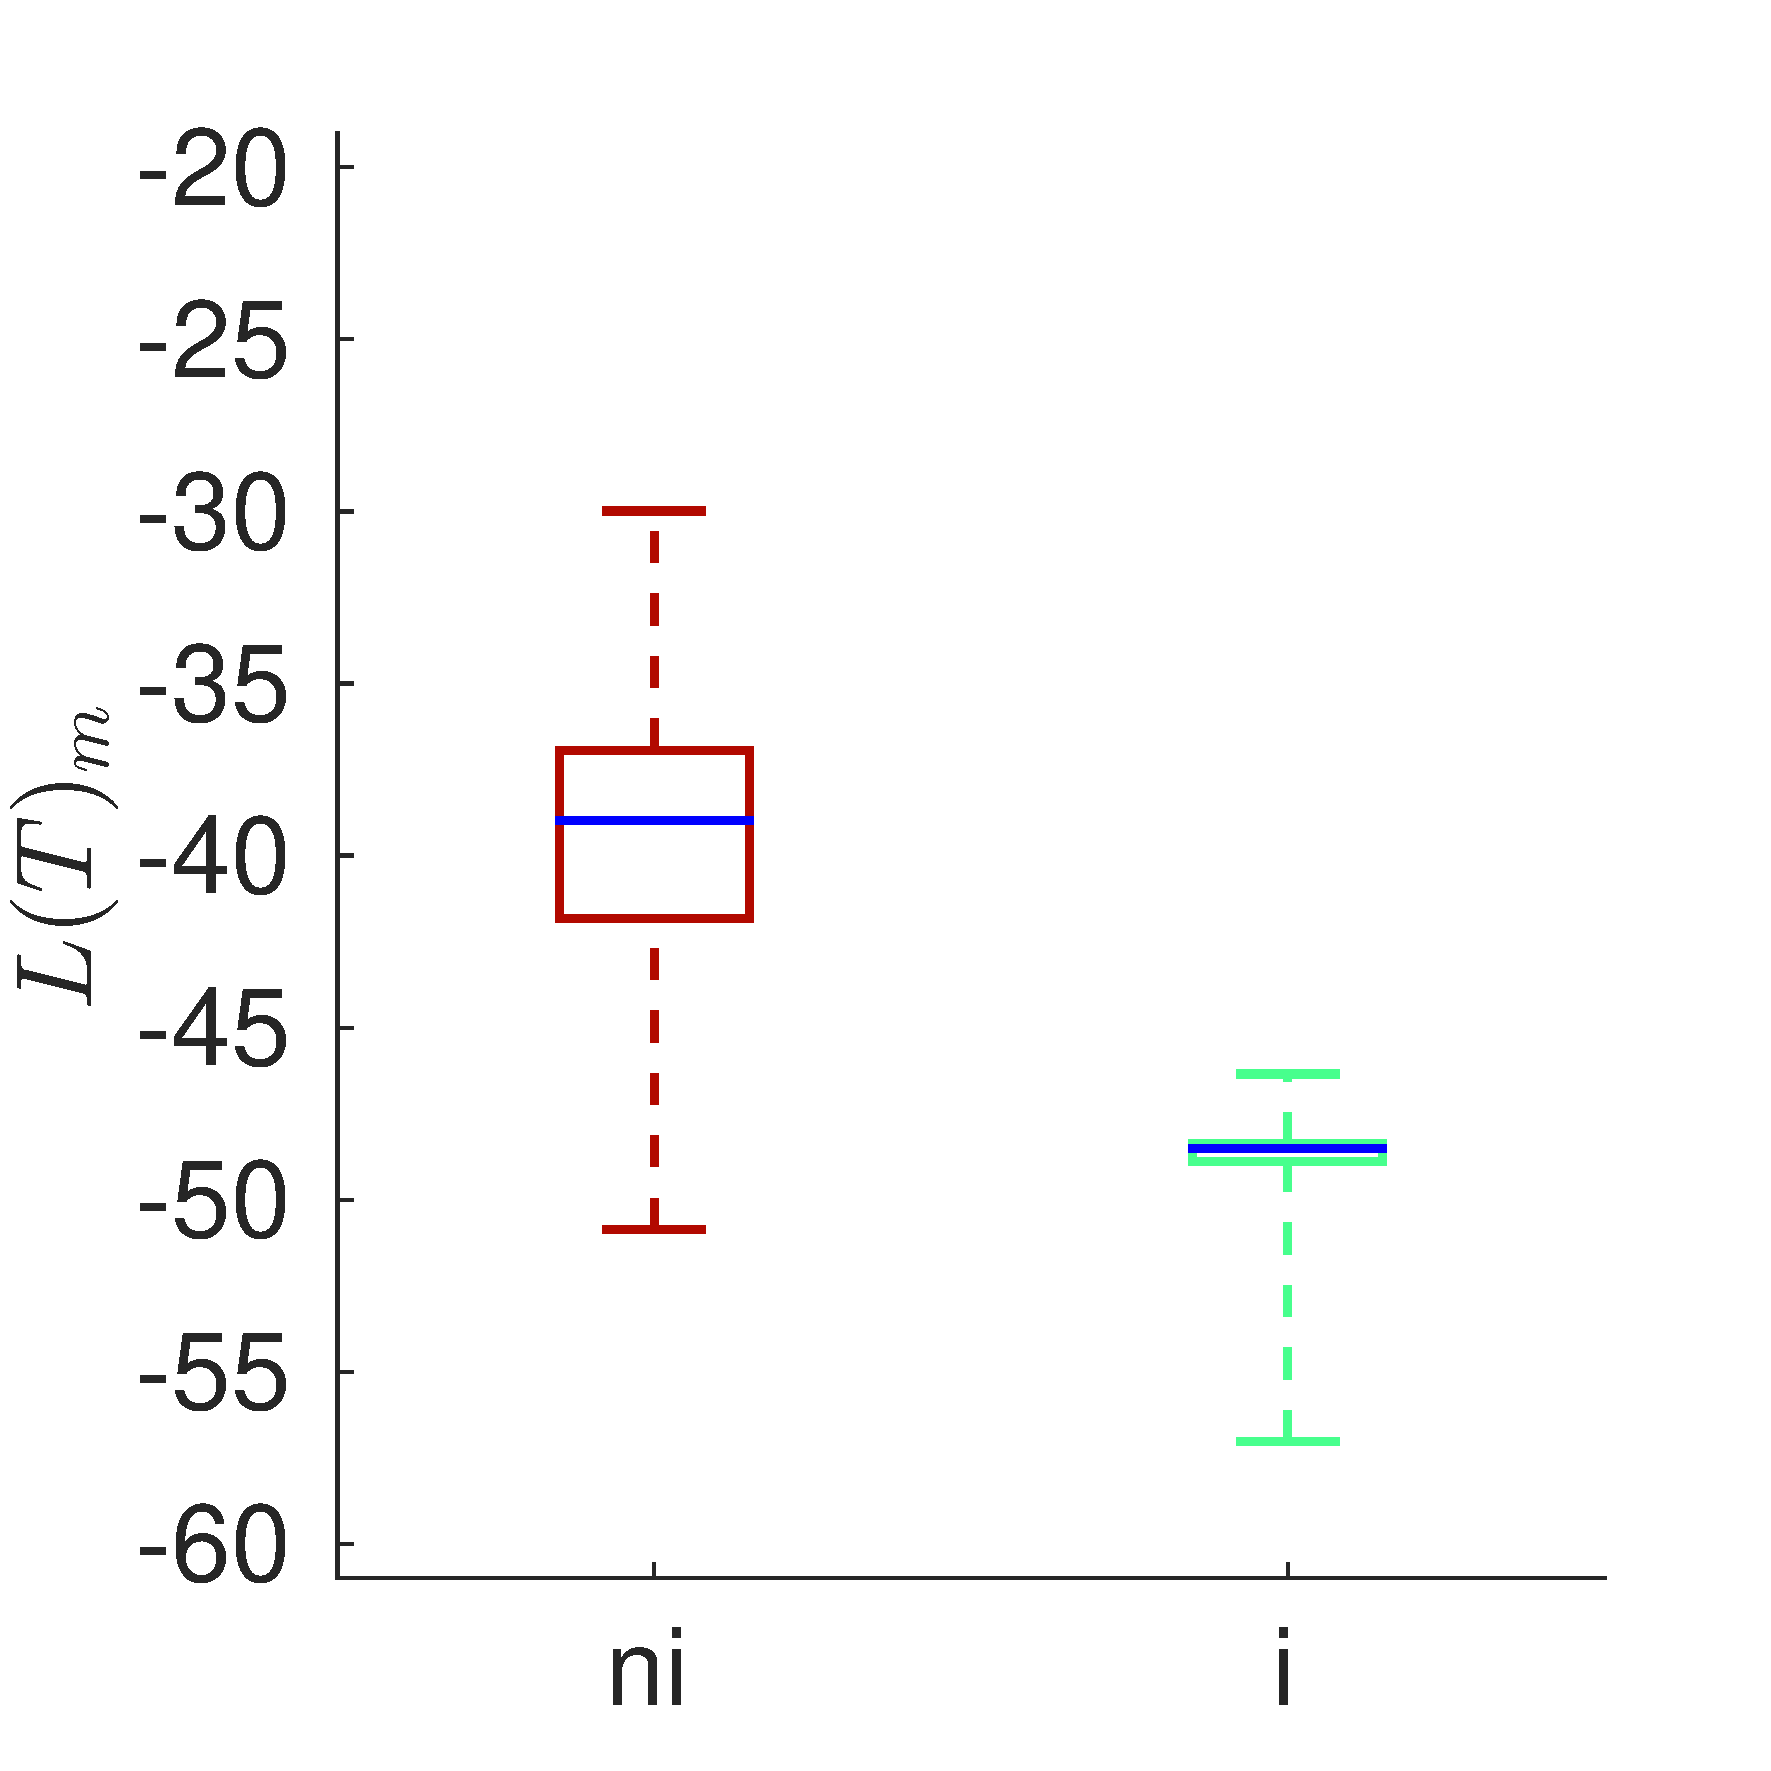
\includegraphics[width=.33\linewidth]{gfxXpUrbanSoundscape/xp_soundlevel_15}\label{fig:soundlevelMarkerc}}\par
        \subfloat[]
        {\includegraphics[width=.33\linewidth]{gfxXpUrbanSoundscape/xp_soundlevel_8}\label{fig:soundlevelMarkerd}}
        \subfloat[]
        {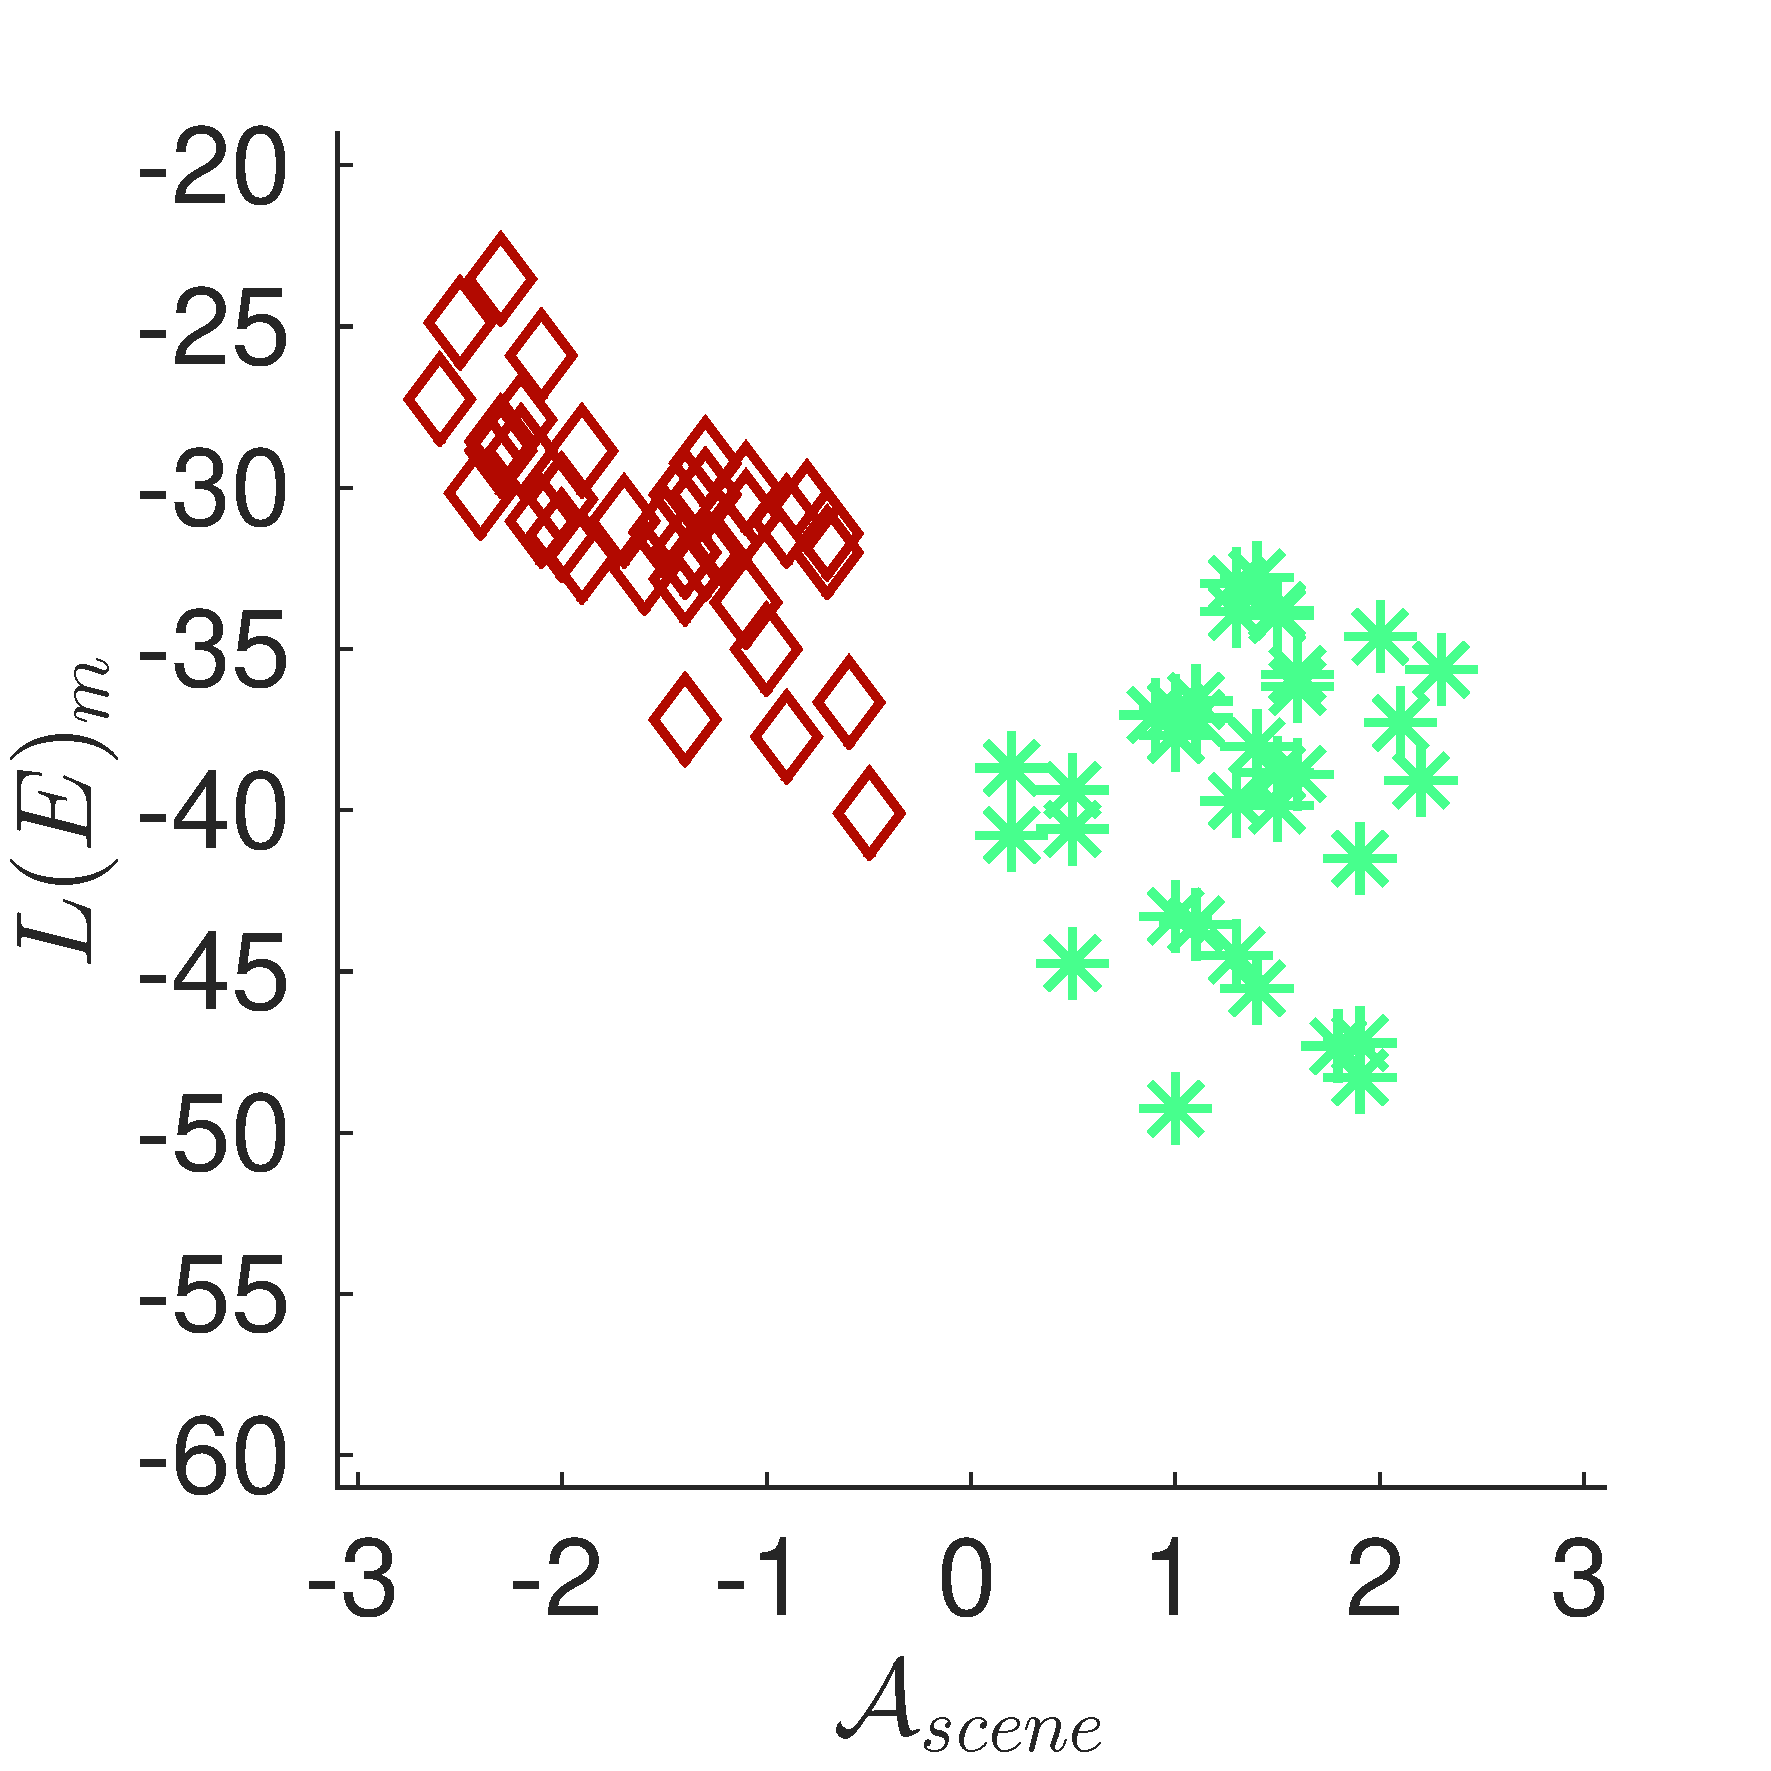
\includegraphics[width=.33\linewidth]{gfxXpUrbanSoundscape/xp_soundlevel_12}\label{fig:soundlevelMarkere}}
        \subfloat[]
        {\includegraphics[width=.33\linewidth]{gfxXpUrbanSoundscape/xp_soundlevel_16}\label{fig:soundlevelMarkerf}}\par
        \subfloat[]
        {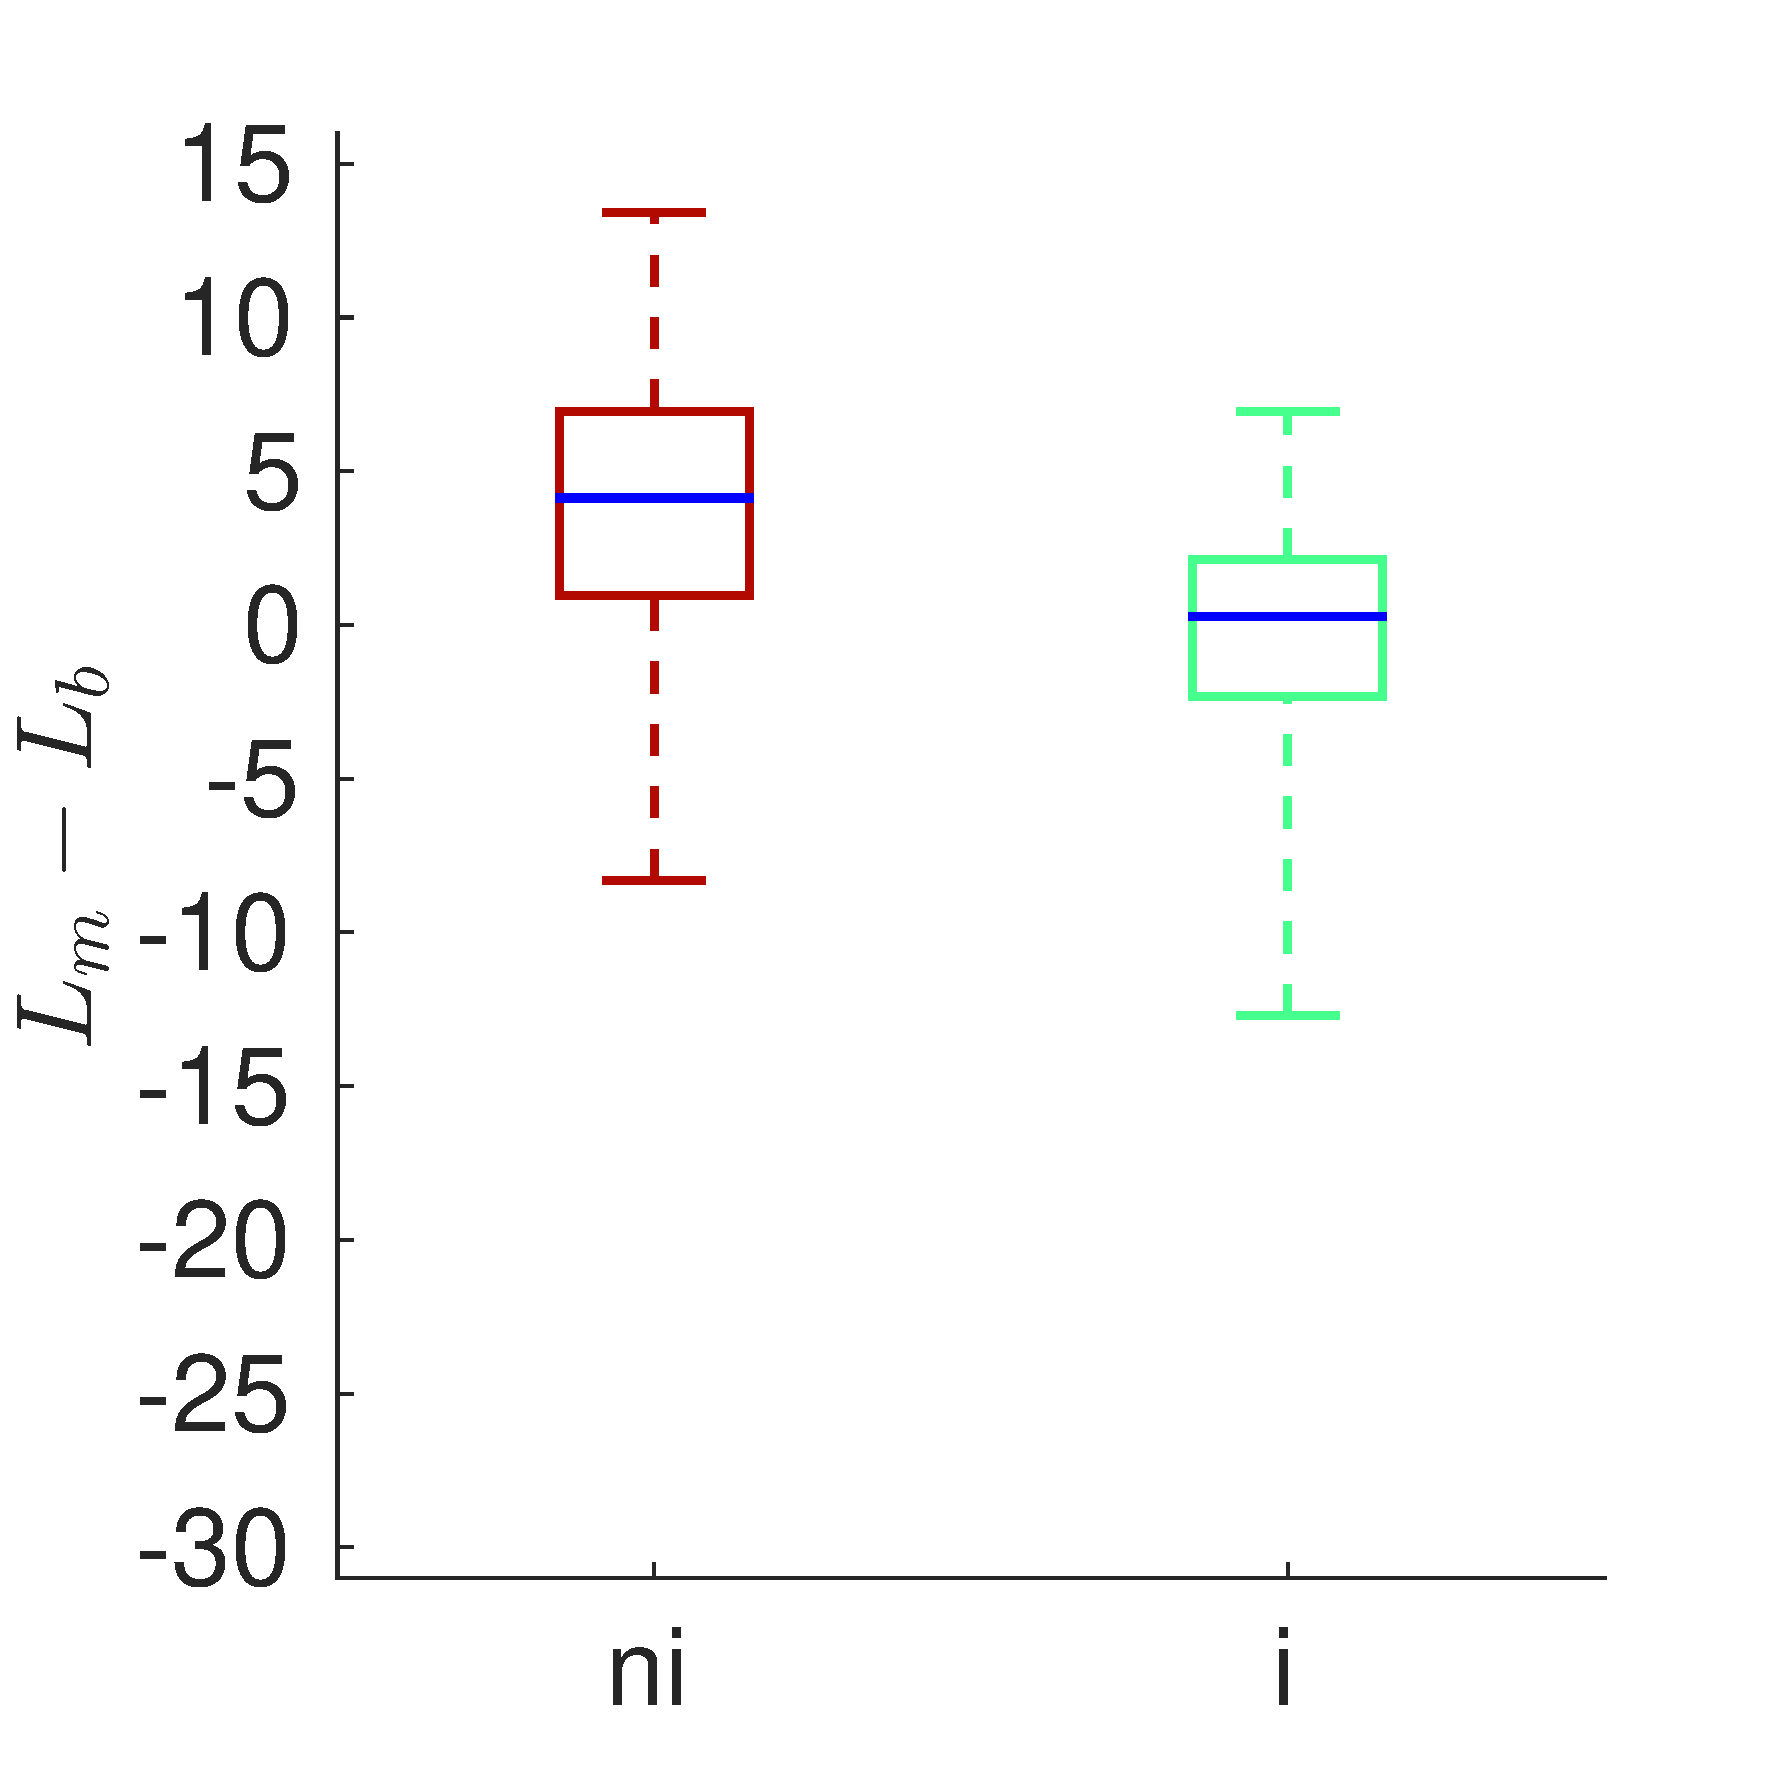
\includegraphics[width=.33\linewidth]{gfxXpUrbanSoundscape/xp_soundlevel_19}\label{fig:soundlevelMarkerDiffa}}
        \subfloat[]
        {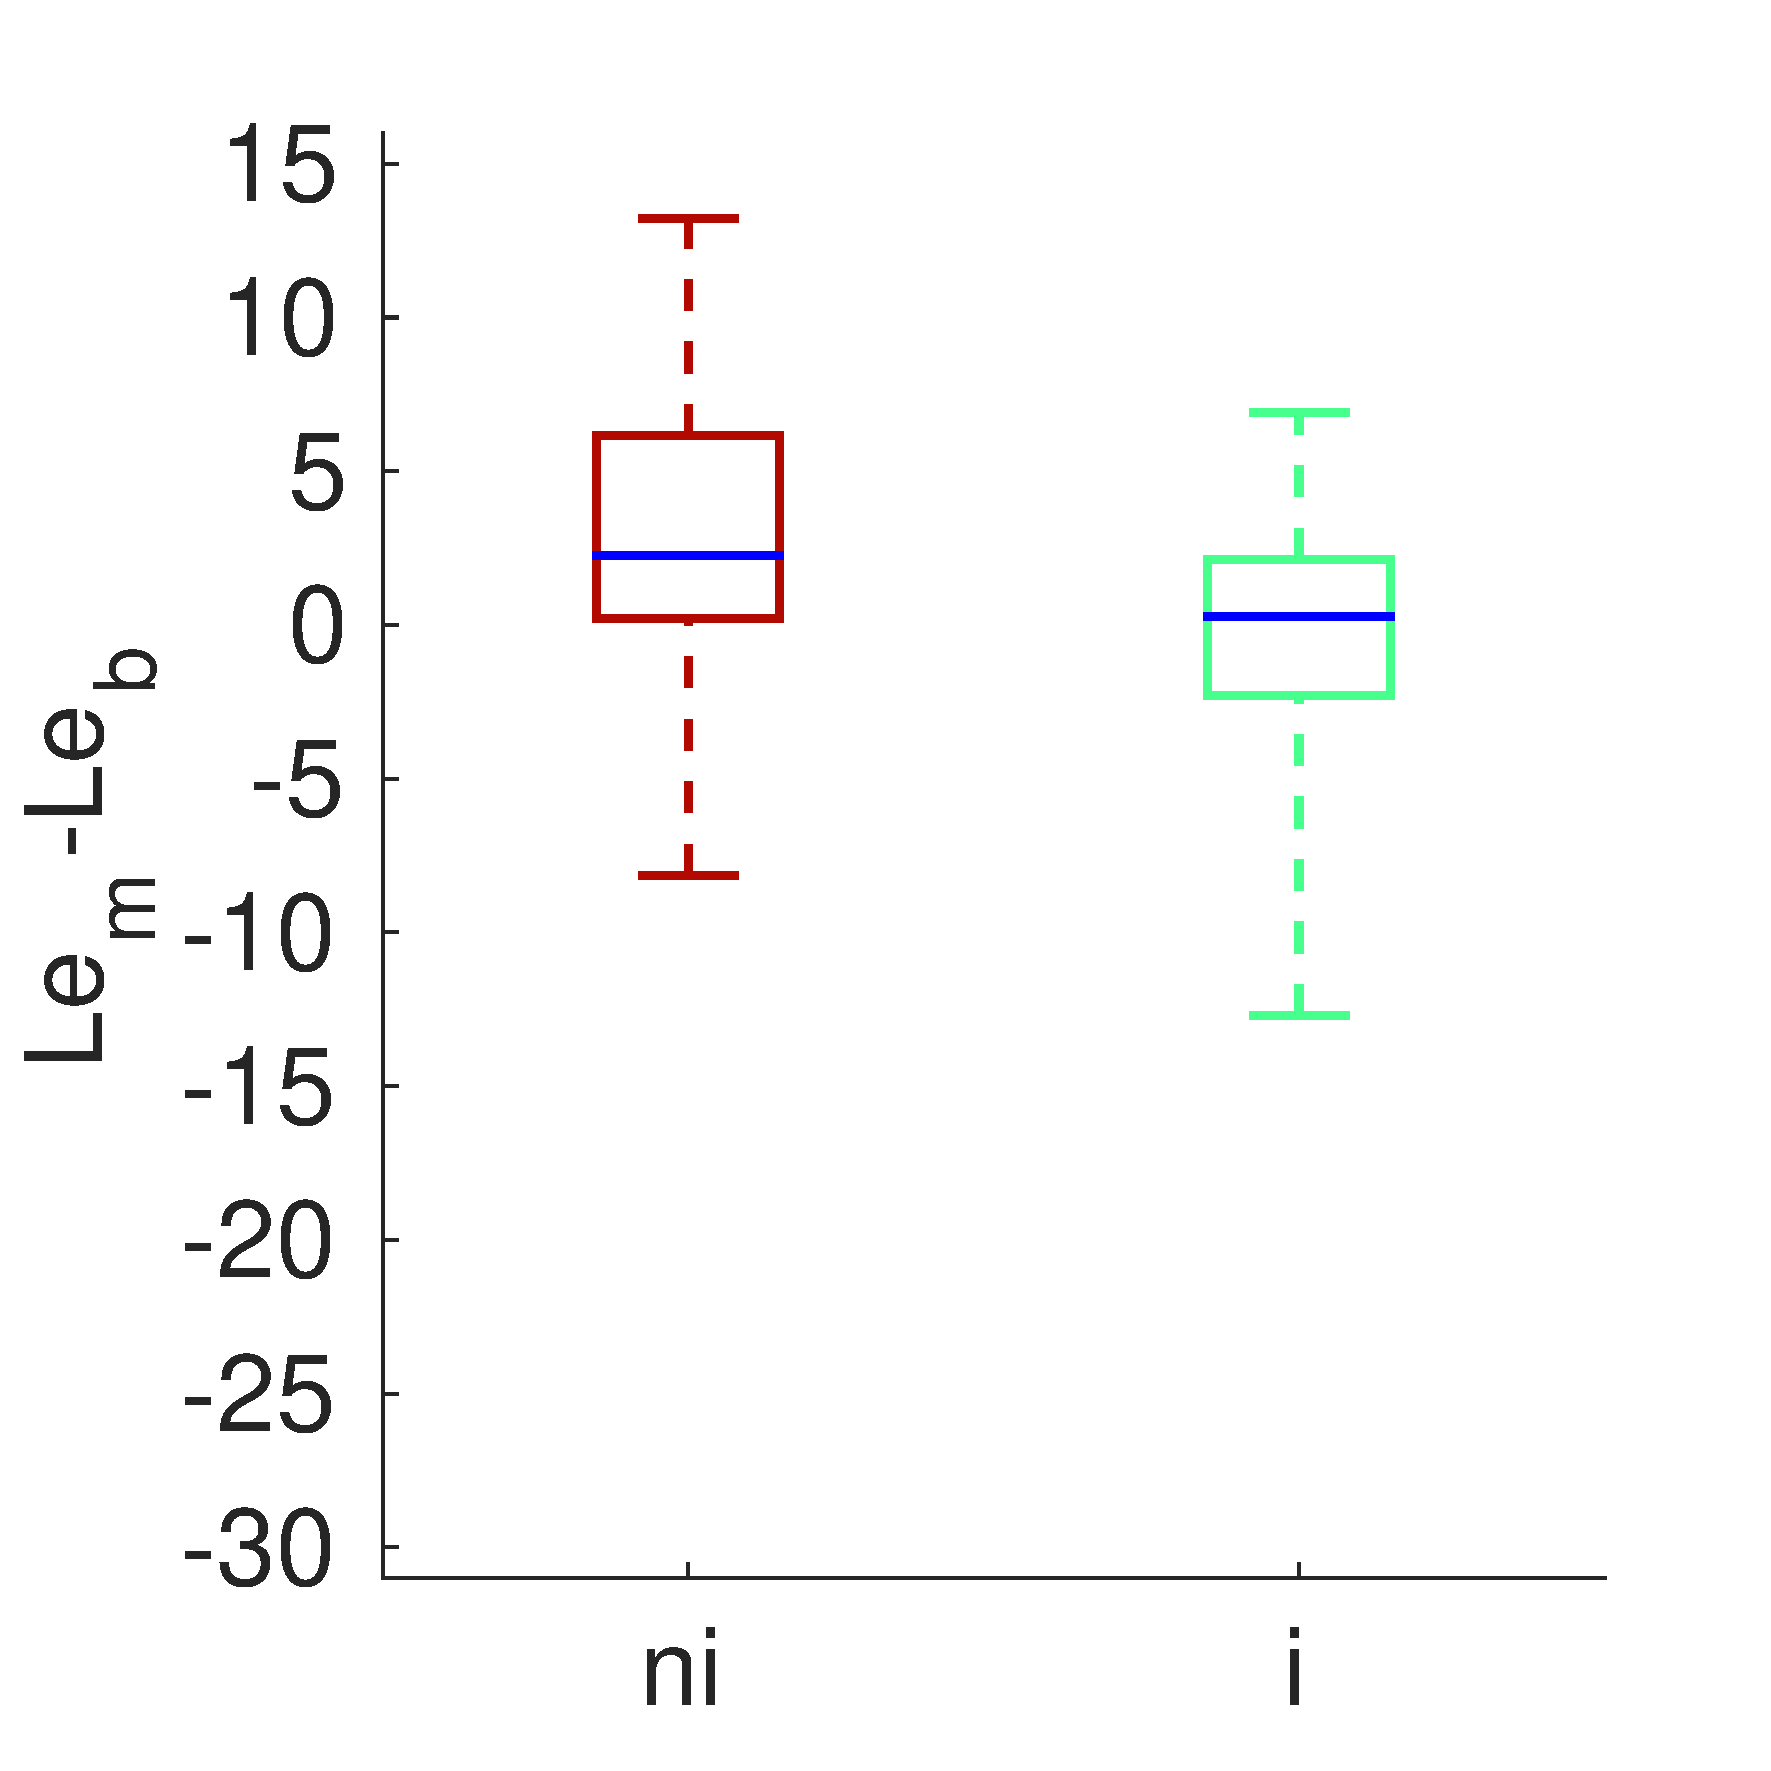
\includegraphics[width=.33\linewidth]{gfxXpUrbanSoundscape/xp_soundlevel_21}\label{fig:soundlevelMarkerDiffb}}
        \subfloat[]
        {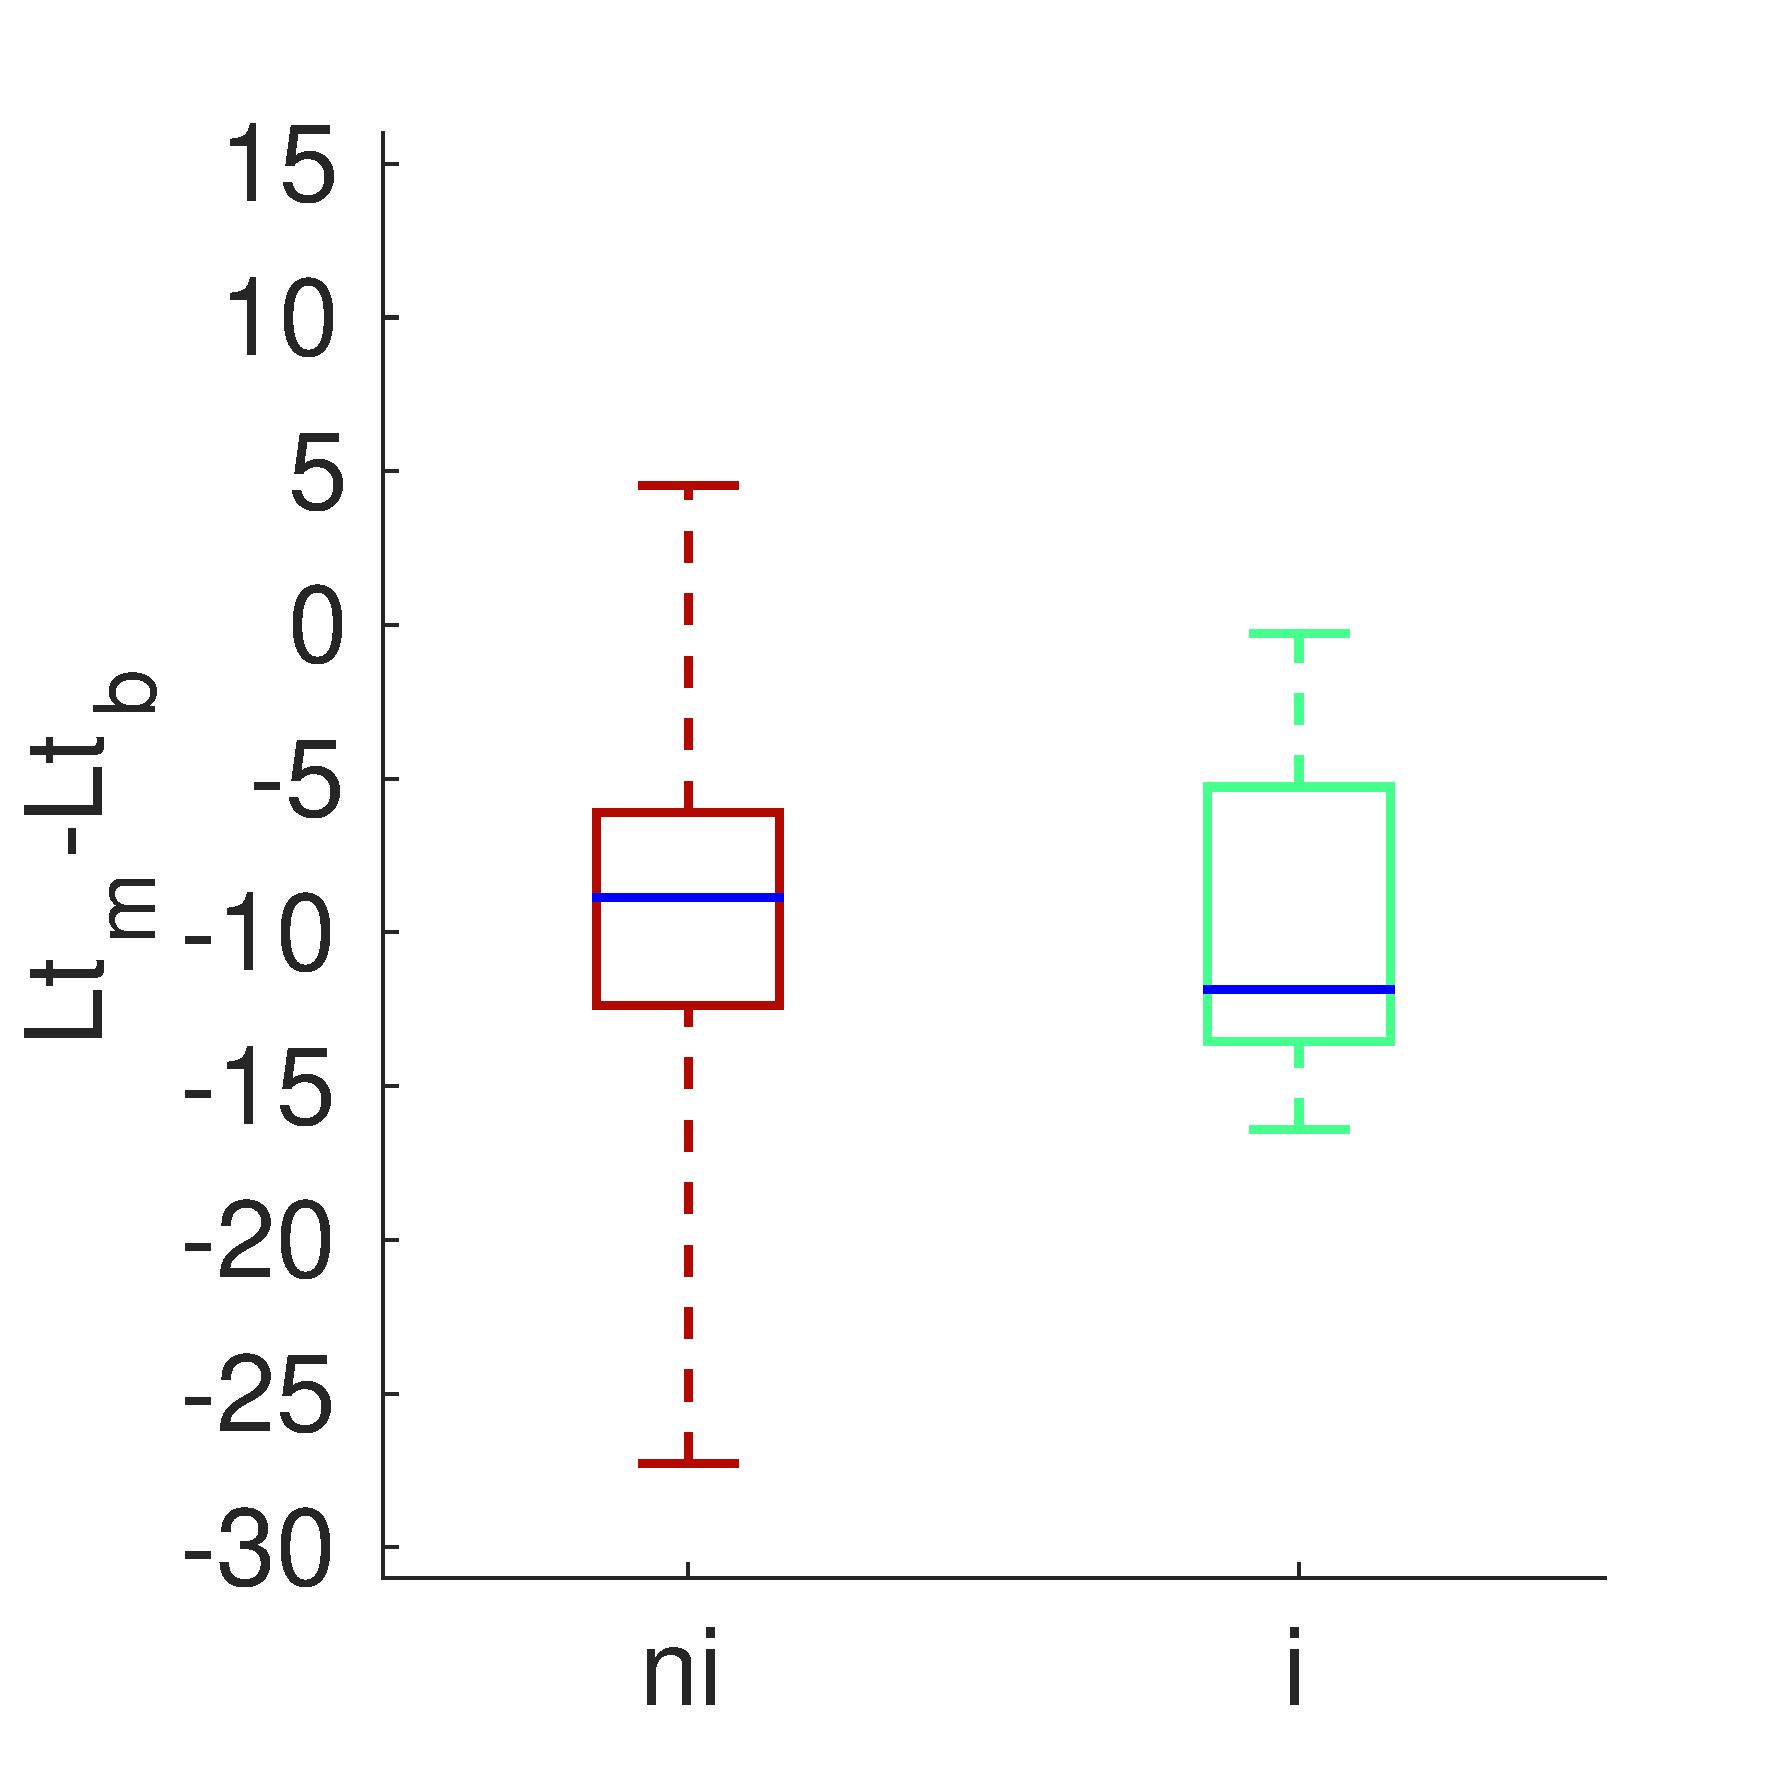
\includegraphics[width=.33\linewidth]{gfxXpUrbanSoundscape/xp_soundlevel_23}\label{fig:soundlevelMarkerDiffc}}\par
        \subfloat[]
        {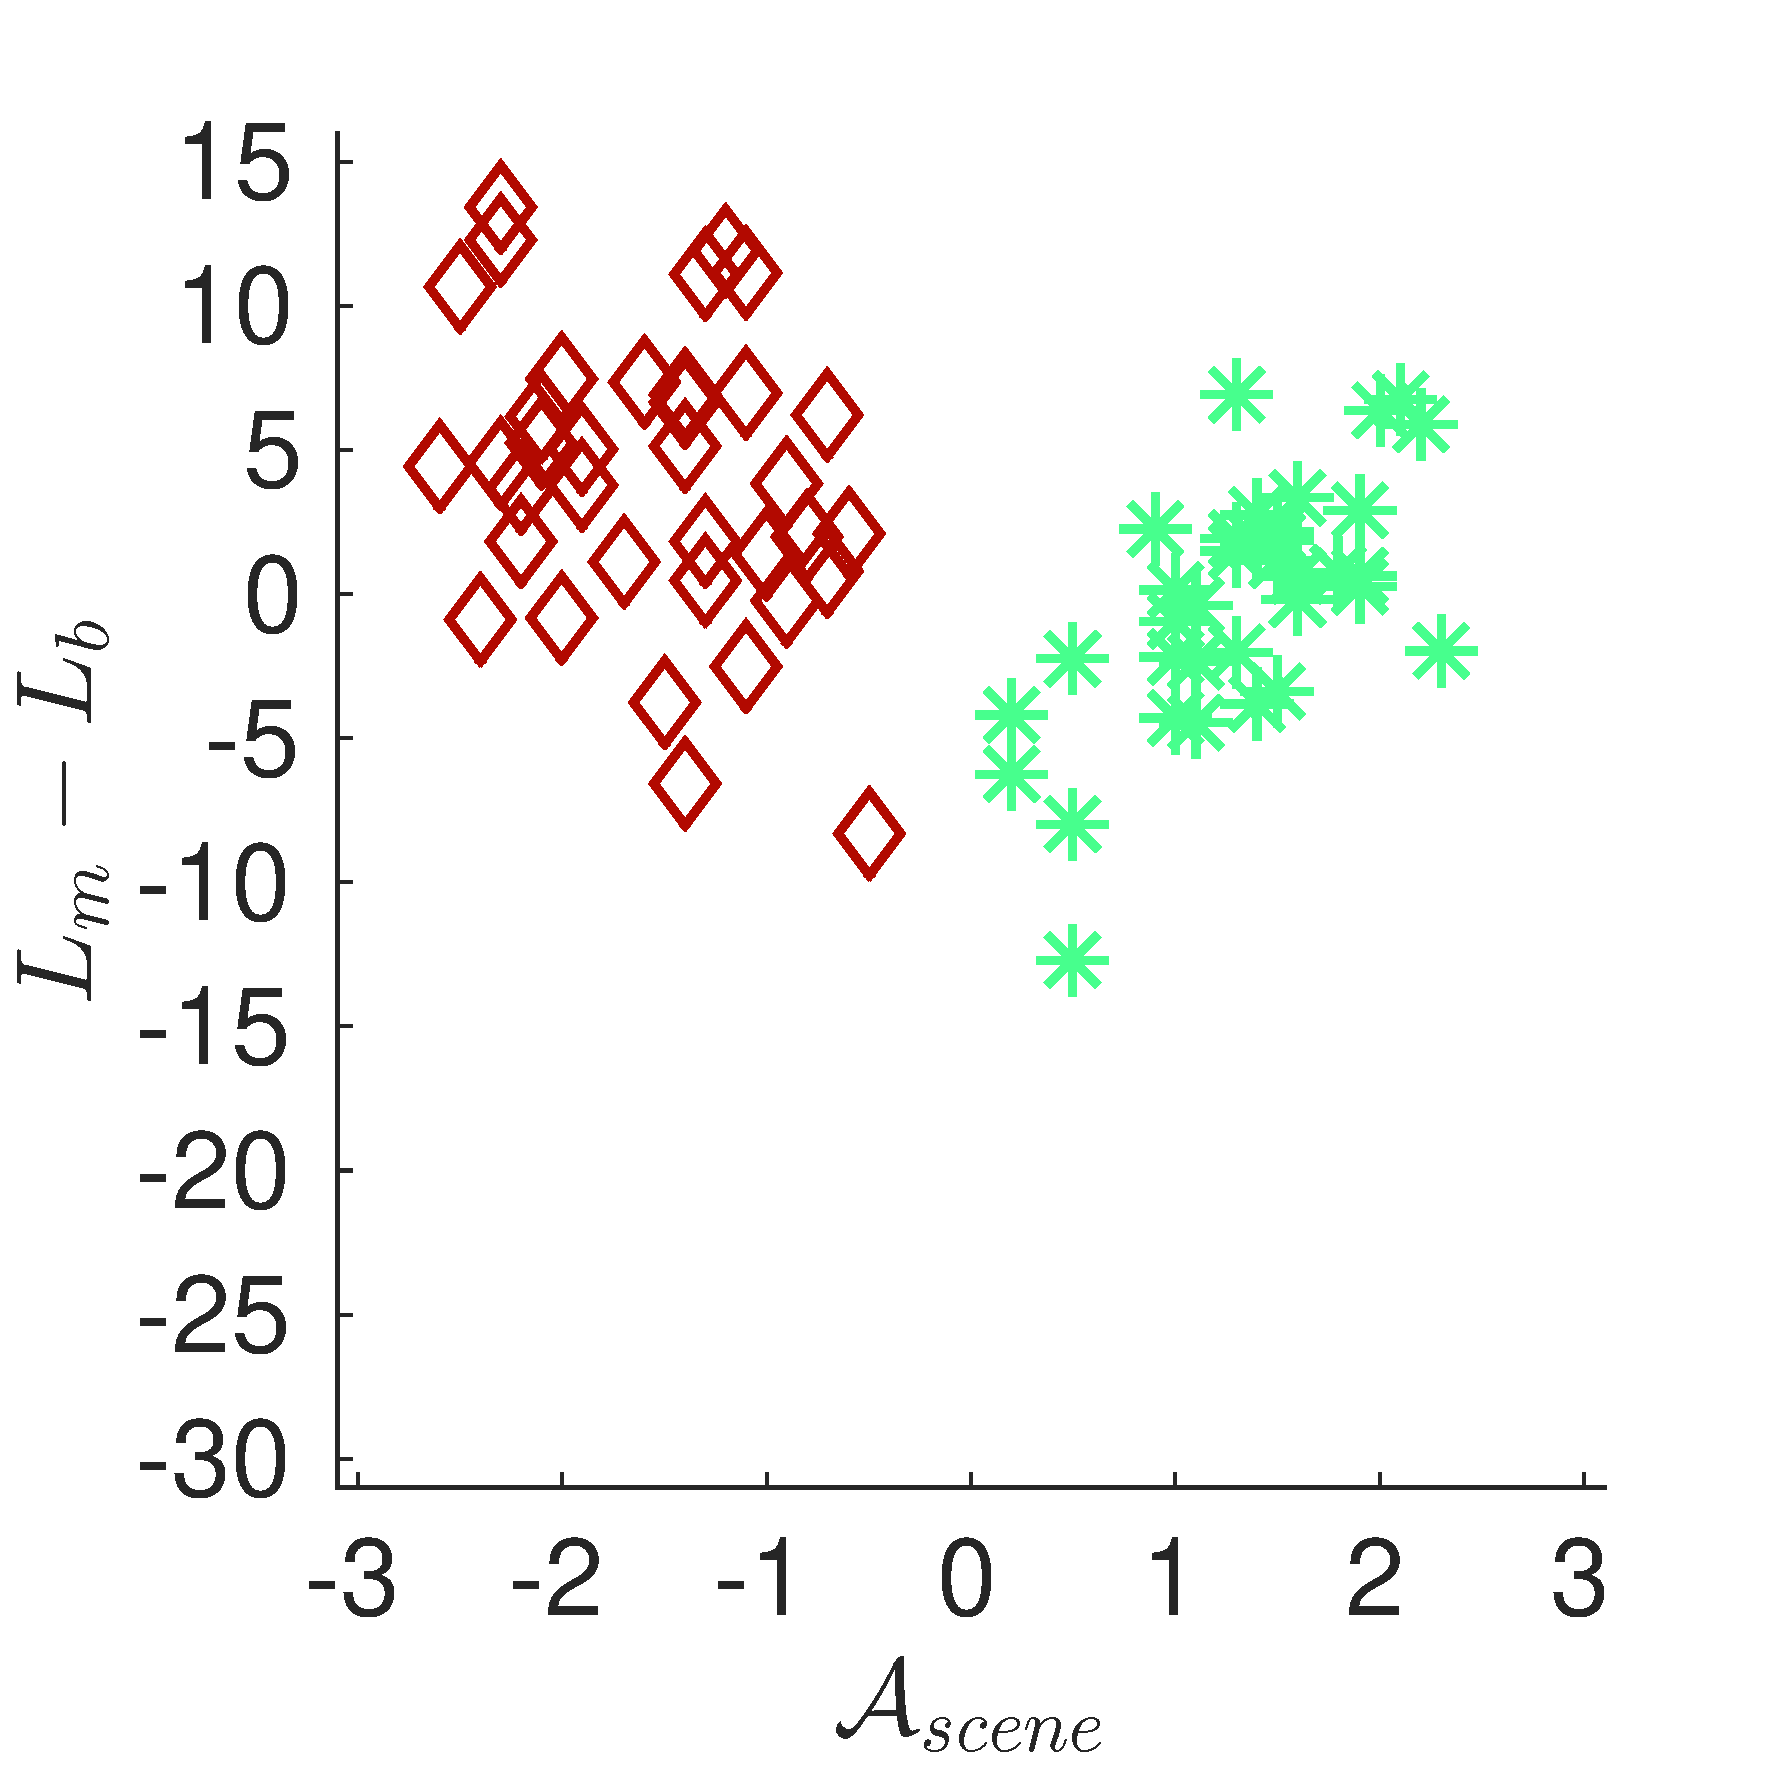
\includegraphics[width=.33\linewidth]{gfxXpUrbanSoundscape/xp_soundlevel_20}\label{fig:soundlevelMarkerDiffd}}
        \subfloat[]
        {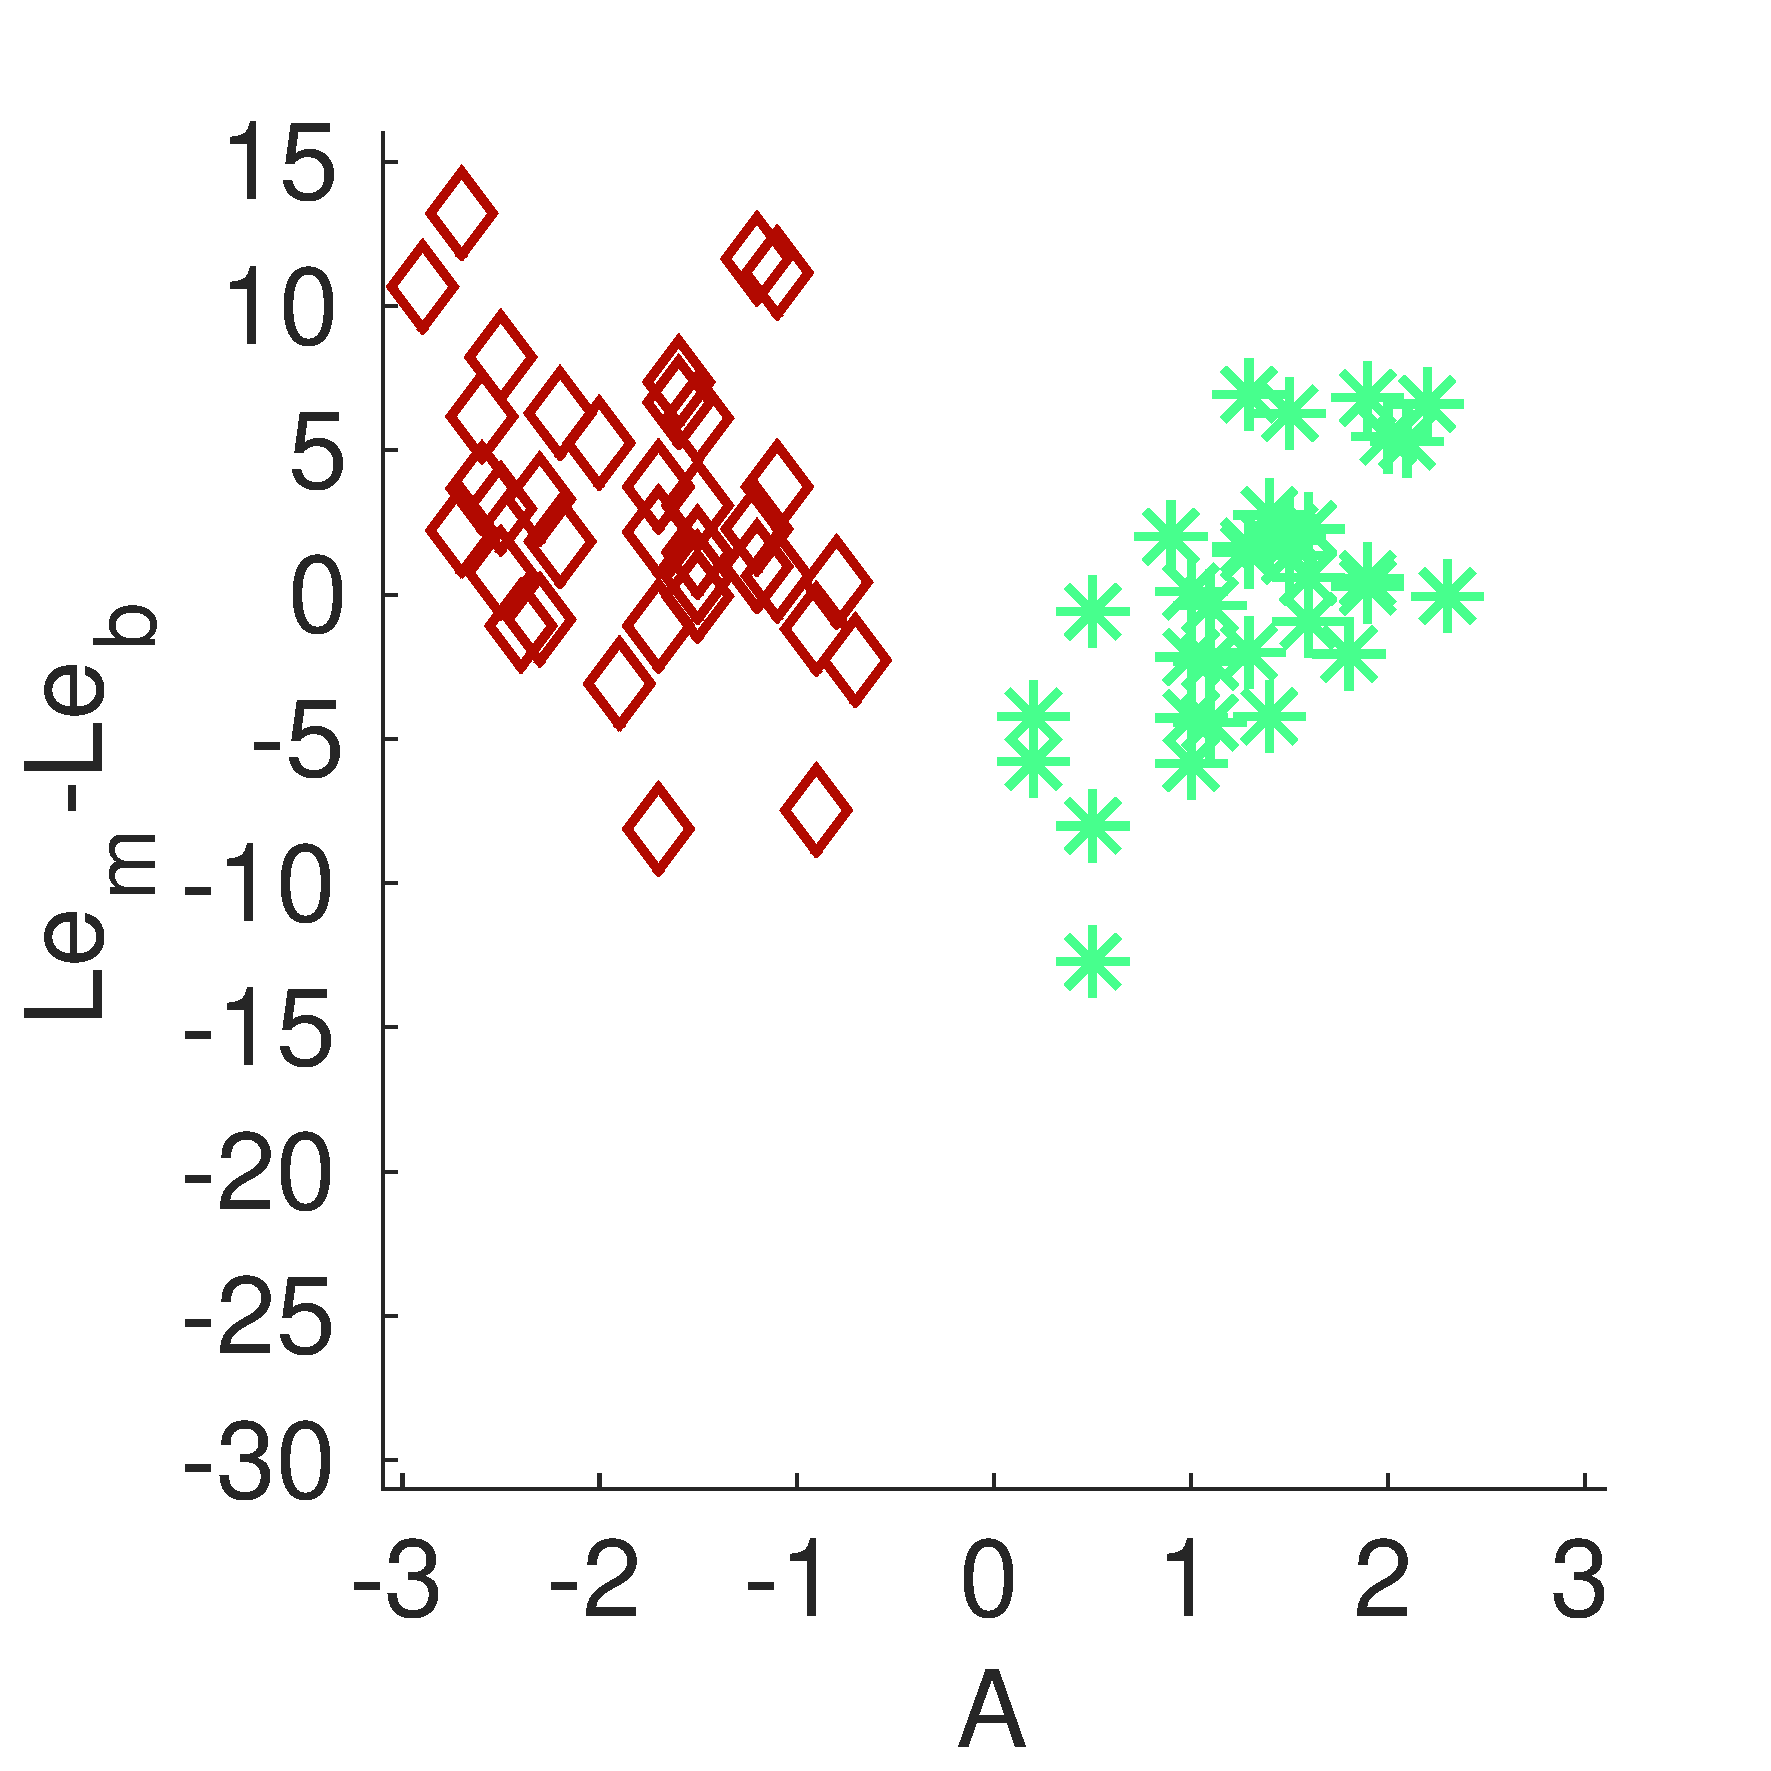
\includegraphics[width=.33\linewidth]{gfxXpUrbanSoundscape/xp_soundlevel_22}\label{fig:soundlevelMarkerDiffe}}
        \subfloat[]
        {\includegraphics[width=.33\linewidth]{gfxXpUrbanSoundscape/xp_soundlevel_24}\label{fig:soundlevelMarkerDifff}}
       \caption[TODO]{TODO}\label{fig:soundlevelMarker}
\end{figure}




\subsection{Discussions}

Nous identifions 6 indicateurs structurels globaux permettant de distinguer, de manière globale, les environnements sonore idéaux et non-idéaux.

\begin{itemize}
\item niveau sonore: calculé sur tous les sons $L$, les événements $L(E)$ et les textures $L(T)$ 
\item densité: calculé de manière globale ($D$) et sur les événements $D(E)$.
\item diversité: calculé uniquement sur les événements $E$
\end{itemize}

Parmi, ces indicateurs structurels, seuls $L$ et $LE$ permettent de prédire l'agrément. Nous notons cependant que cette prédiction ne vaut que pour les ni-scènes. 

Nous observons qu'une description sémantique des scènes, basée sur la présence/absence des classes de sons, permet de bien prédire la nature de l'environnement. Par ailleurs, il apparaît qu'il est possible d'obtenir une prédiction similaire, voire meilleure, en ne considérant qu'un sous groupe de classes d'événements,\ie~les marqueurs sonores.

Parmi les descripteurs structurels spécifiques, calculés en tenant compte des marqueurs sonores, \jlv{X} \jls{plusieurs} permettent maintenant de faire la distinction entre les i-scènes et ni-scènes:

\begin{itemize}
\item X
\end{itemize}

Parmi ces descripteurs, 5 sont capables de prédire l'agrément de manière fine: 

\begin{itemize}
\item $L(E)_m-L(E)_b$ et $L_m-L_b$ pour les i-scènes
\item 
\end{itemize}

De cette analyse, nous retenons les points suivant:

\begin{itemize}
\item \emph{Distinguer les i- et ni-scènes}: Les descripteurs sémantiques, ainsi que certains descripteurs structurels globaux, permettent de faire la distinction entre les i-scènes et les ni-scènes. La description sémantique semble être plu performante.
\item \emph{Événements ou textures}: Que ce soit pour les descripteurs sémantiques ou structurels, c'est majoritairement les événements qui permettent de distinguer les deux types d'environnements, les textures n'apportant au mieux qu'une information limitée.
\item \emph{Prédire l'agrément}: Si l'on considère une description fine de l'agrément, il semble que la manière de percevoir la qualité de l'environnement diffère en fonction de la nature de ce dernier (i ou ni). Il \jlv{ne semble pas} \jls{il n'apparaît pas} envisageable de considérer un même jeu de descripteurs pour prédire à la fois l'agrément des i-scènes et l'agrément des ni-scènes. Pour les ni-scènes, c'est le niveau global ($L$ et $L(E)$), la densité globale ($D$ et $D(E)$), ou encore le niveau des marqueurs sonores ($L_m$ et $L$), qui impactent négativement l'agrément. On note ici que prendre en compte les contributions de différentes sources n'améliore pas la capacité de prédiction de l'agrément, par rapport à une analyse holistique de l'environnement. Pour les i-scènes, par contre, prédire l'agrément requiert d'étudier de manière séparée les caractéristiques des marqueurs sonores et du reste des sons. Ainsi le niveau des marqueurs relatifs au bruit est positivement corrélé à l'agrément, alors que le niveau du bruit est, lui, négativement corrélé.  
\end{itemize}

L'existence de deux modes de perceptions, engageant \jls{ou mobilisant, ou encore mettant en œuvre} différents types de descripteurs, et dépendant de la nature du stimuli, est un phénomène qui a déjà été observé pour la perception des textures (\cf~section~\ref{sec:ch3_eventTexture}). Le cerveau adapte sa manière de traiter l'information (résumé statistique pour les textures, description fine pour les événements) suite à une prise de décision antérieure quant à la nature du stimuli (à savoir ``\,est-ce un événement ou une texture ?\,''). De la même manière, les indicateurs actifs dans le jugement de l'agrément dépendent eux aussi de l'identification préalable de la nature globale de ce dernier \jlc{"ce dernier" renvoie à quel mot ? stimuli ? pour la compréhension il faut le repréciser ici} (idéale ou non idéale).

Ces résultats peuvent potentiellement influer sur les stratégies à adopter pour améliorer la qualité de l’environnement sonore:

\begin{itemize}
\item Dans le cadre de scènes non-idéales, il s'agit de diminuer le niveau sonore, soit de manière globale, soit en agissant sur certaines sources (\emph{sirène}, \emph{klaxon}). 
\item Dans le cadre de scènes idéales, il s'agit 1) d'identifier les sons agréables, \ie~les marqueurs sonores, 2) de baisser le niveau des autres sons, 3) voire, en restant dans la limite du raisonnable, d'augmenter le niveau des marqueurs par rapport aux autres sons.
\end{itemize}

Nous montrons que les descripteurs à utiliser dépendent de la nature de l'environnement, \jlv{et que cette nature est largement dépendante de la composition sémantique, \ie~des sources sonores présentes} \jls{et que cette nature est elle même dépendante de la composition sémantique, \ie~des sources sonores présentes}. Dans une certaine mesure, nous pouvons donc dire que les descripteurs dépendent des sources sonores présentes. Mais nous observons également que le type de descripteurs à utiliser varie pour une même source \jlv{ayant été utilisée dans les deux types d'environnements} \jlc{cela est mal dit, et mérite d'être reformulé} (\gl{développer sur le contexte environnemental pour l'agrément, reprendre l'exemple de \emph{foule}}). \\

\gl{Reprendre la conclusion de l'article et Proposer un modèle perceptif sur la base du modèle prédictif}

\section{Agir sur l'agrément perçu en modifiant la composition sémantique}
\label{sec:xp3}

\subsection{Objectif de l'expérience}

\subsection{Planification expérimentale}

\subsection{Données et méthodes d'analyses}

\subsection{Discussions}

\section{L'impact de la composition sur les processus de catégorisation des scènes}
\label{sec:xp4}

\subsection{Objectif de l'expérience}

\subsection{Planification expérimentale}

\subsection{Données et méthodes d'analyses}

\subsection{Discussions}
%*****************************************
%*****************************************
%*****************************************
%*****************************************
%*****************************************




